%% packages
\documentclass{article}
\usepackage[a4paper, left=2.0cm, right=2.0cm, top=3.5cm]{geometry}
\usepackage[ngerman]{babel}
\usepackage{graphicx}
\usepackage{multicol}
\usepackage{amssymb}
\usepackage{titlesec}
\usepackage{wrapfig}
\usepackage{blindtext}
\usepackage{lipsum}
\usepackage{caption}
\usepackage{listings}
\usepackage{fancyhdr}
\usepackage{nopageno}
\usepackage{authblk}
\usepackage{amsmath} % tons of math stuff
\usepackage{mathtools} % e.g. alignment within matrix
%\usepackage{bm} % provides shorthand for bold in math mode
\usepackage{dsfont} % \mathds makes double stroke digits
\usepackage{esdiff} % provides \diff
%\usepackage[ISO]{diffcoeff}
\usepackage{xcolor}
\usepackage{csquotes} % e.g. provides \enquote
\usepackage[separate-uncertainty=true]{siunitx} % units
\usepackage{xcolor} % colored text
\usepackage{csvsimple}
\usepackage{subcaption}
\usepackage{physics}
\usepackage{hyperref}
\usepackage{nameref}
\hypersetup{colorlinks=true, linkcolor=black, pdfhighlight={/N}}
\usepackage{tcolorbox}
\usepackage{amsthm}
\usepackage{float}
\usepackage{enumitem}
\usepackage{booktabs}




%\fancyhf[]{}

%% custom stuff
% own units
\DeclareSIUnit \VSS {\ensuremath{V_\mathrm{SS}}}
\DeclareSIUnit \VS {\ensuremath{V_\mathrm{S}}}
\DeclareSIUnit \Veff {\ensuremath{V_\mathrm{eff}}}
\DeclareSIUnit \Vpp {\ensuremath{V_\mathrm{pp}}}
\DeclareSIUnit \Vp {\ensuremath{V_\mathrm{p}}}
\DeclareSIUnit \VRMS {\ensuremath{V_\mathrm{RMS}}}
\DeclareSIUnit \ASS {\ensuremath{A_\mathrm{SS}}}
\DeclareSIUnit \AS {\ensuremath{A_\mathrm{S}}}
\DeclareSIUnit \Aeff {\ensuremath{A_\mathrm{eff}}}
\DeclareSIUnit \App {\ensuremath{A_\mathrm{pp}}}
\DeclareSIUnit \Ap {\ensuremath{A_\mathrm{p}}}
\DeclareSIUnit \ARMS {\ensuremath{A_\mathrm{RMS}}}

% change subsection numbering to capital letters
\newcommand{\subsectionAlph}{ \renewcommand{\thesubsection}{\arabic{section}.\Alph{subsection}} }
% change subsection numbering to lowercase letters
\newcommand{\subsectionalph}{ \renewcommand{\thesubsection}{\arabic{section}.\alph{subsection}} }
% change subsubsection numbering to lowercase letters
\newcommand{\subsubsectionalph}{ \renewcommand{\thesubsubsection}{\arabic{section}.\arabic{subsection}.\alph{subsubsection}} }
% own fig. that works with multicols
\newenvironment{Figure}
  {\par\medskip\noindent\minipage{\linewidth}}
  {\endminipage\par\medskip}
\newcommand*{\inputPath}{./plot} % prepend this command to the argument of all input commands
\graphicspath{ {./images/}{./figure/}{../plot/} }
% own enviroment for definitions
\newenvironment{definition}[1]
{\begin{quote} \noindent \textbf{\textit{#1\ifx&#1& \else : \fi}} \itshape}
{\end{quote}}


% own commands
% \newcommand{\rarr}{$\to\,$} %A$\,\to\,$B
\newcommand{\defc}{black}
\newcommand{\colorT}[2][blue]{\color{#1}{#2}\color{\defc}}
\newcommand{\redq}{\color{red}(?)\color{\defc}}
% \newcommand{\question}[1]{\colorT[purple]{\textbf{(#1)}}}
\newcommand{\todo}[1]{\colorT[red]{(#1)}}
\newcommand{\mr}{\mathrm}

%% preparation
\begin{titlepage}
  \title{Praktikum Atome, Moleküle, kondensierte Materie \\ Versuch 401: Elektronische Übergänge in Atomen}
  \author[1]{Carlos Pascua\thanks{s87cpasc@uni-bonn.de}}
  \author[1]{Michael Vogt\thanks{s65mvogt@uni-bonn.de}}
  \affil[1]{Uni Bonn}
  %\date{\today}
\end{titlepage}


%% document
\begin{document}

\pagenumbering{gobble}
\maketitle
\tableofcontents
\newpage
\pagenumbering{arabic}

\pagestyle{fancy}
\fancyhead[R]{\thepage}
\fancyhead[L]{\leftmark}

\begin{multicols}{2}

\section*{Einleitung}
In diesem Versuch wird die Energieaufspaltung von Energie-Niveaus in Cadmium durch den Zeeman-Effekt untersucht.
Daraus wird das Bohrsche Magneton bestimmt sowie Eigenschaften des verwendeten Fabry-Perot-Etalons errechnet.

Anschließend wird das Franck-Hertz-Experiment durchgeführt, um die Energiedifferenz zwischen dem 6S- und 6P-Zustand von Quecksilber zu bestimmen.


\section{Zeeman-Effekt}
Im ersten Versuchsteil wird anhand einer Cadmiumlampe in einem Magnetfeld der Zeeman-Effekt untersucht und
anhand der Ergebnisse das Bohrsche Magneton $\mu_B$ bestimmt.
% Daran soll das Bohrsche Magneton $mu_B$ bestimmt werden.

Der Zeeman-Effekt ist die Aufspaltung von Energieniveaus der Elektronen in Atomen in Abhängigkeit der Magnetquantenzahl $m_J$,
die auftritt, wenn ein äußeres Magnetfeld $B$ anliegt. Die Energie ändert sich wie folgt:
\[
  E = E_C + \mu_B B \cdot m_J
\]
Dabei ist $E_C$ das Energieniveau, das nur von der Coulomb-Wechselwirkung abhängt und keine $m_J$-Abhängigkeit hat.
Für die Energiedifferenz zwischen zwei Übergängen $1$ und $2$ mit unterschiedlichen Magnetquantenzahlen $\Delta m_J = m_J^2 - m_J^1$
gilt dann
\[
  E_2 - E_1 = \Delta E_C + \mu_B B \cdot \Delta m_J
\]
Das abgestrahlte Licht solcher Übergänge hat also eine Energieverschiebung in Abhängigkeit von $\Delta m_J$ und $B$.
Die Energieverschiebung eines Übergangs mit angelegtem Magnetfeld im Vergleich zu keinem Magnetfeld bezeichnen wir im Folgenden mit $\Delta E$:
\begin{equation}
  \Delta E = E_2 - E_1 - \Delta E_C = \mu_B B \cdot \Delta m_J \label{eq:delta-e}
\end{equation}

Je nach dem Wert von $\Delta m_J$ werden Übergänge unterschiedlich bezeichnet:
$\Delta m_J=0$ ist ein $\pi$-Übergang und $\Delta m_J=\pm 1$ sind $\sigma^\pm$.
Diese haben unterschiedliche Polarisierungen und Abstrahlungscharakteristiken, die in Abb. \ref{fig:zeeman-abstrahlung}
gezeigt sind.
\begin{figure}[H]
  \centering
  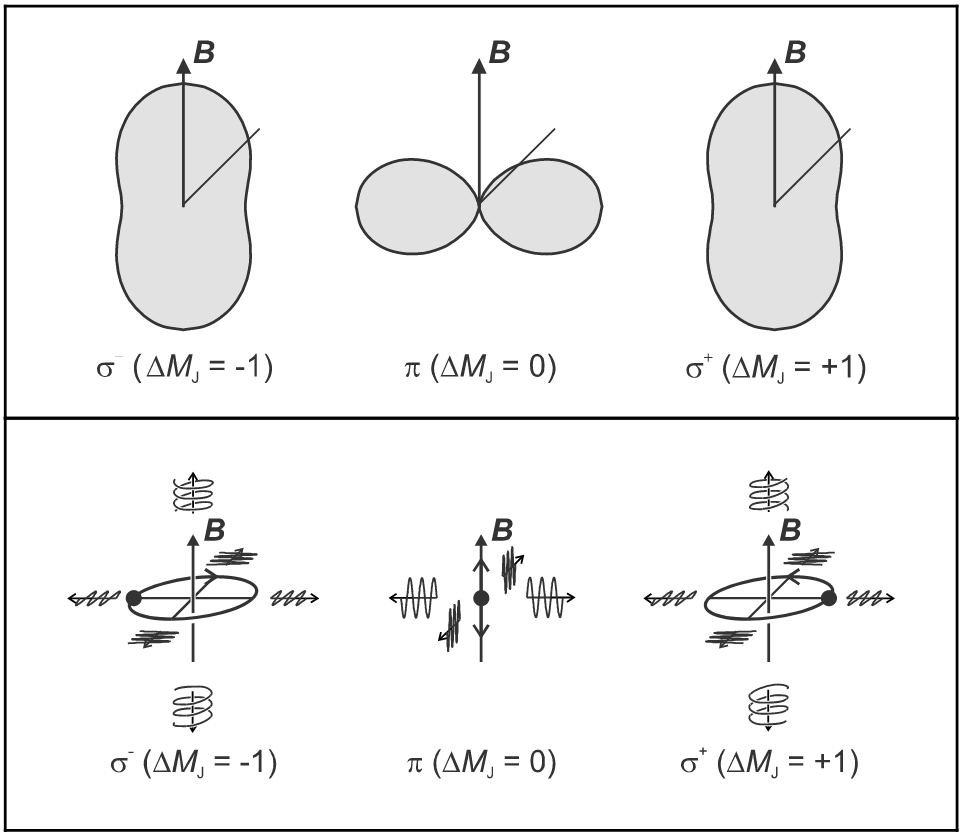
\includegraphics[width=.8\linewidth]{zeeman-abstrahlung}
  \caption{Polarisationsverteilung und Abstrahlungscharakteristik elektrischer Dipolübergänge \cite{Anleitung} \cite{Leybold}.
    Die kreisende bzw. schwingende Kugel in der unteren Hälfte ist ein klassisches Analogon für das Verhalten des Elektrons.
    Dadurch lassen sich die Polarisationen der Strahlung in verschiedenen Richtungen (in der Unteren Hälfte gezeigt)
    sowie die allgemeine Strahlungscharakteristik (in der oberen Hälfte) erklären.}
  \label{fig:zeeman-abstrahlung}
\end{figure}
Hier ist zu sehen, dass ein $\pi$-Übergang bei longitudinaler Betrachtung (Blickrichtung parallel zum B-Feld) nicht zu sehen ist
und das Licht der $\sigma$-Übergänge hier in entgegengesetzten Richtungen zirkular polarisiert ist.
Bei transversaler Betrachtung (senkrecht zum Magnetfeld) sind alle Übergänge zu sehen und sind linear polarisiert.
Die $\sigma$-Übergänge erzeugen gleiche Polarisationsrichtung, die senkrecht zu der des $\pi$-Übergangs steht.

\subsection{Aufbau}
Der verwendete Aufbau ist in Abb. \ref{fig:zeeman-aufbau} zu sehen.
\begin{figure}[H]
  \centering
  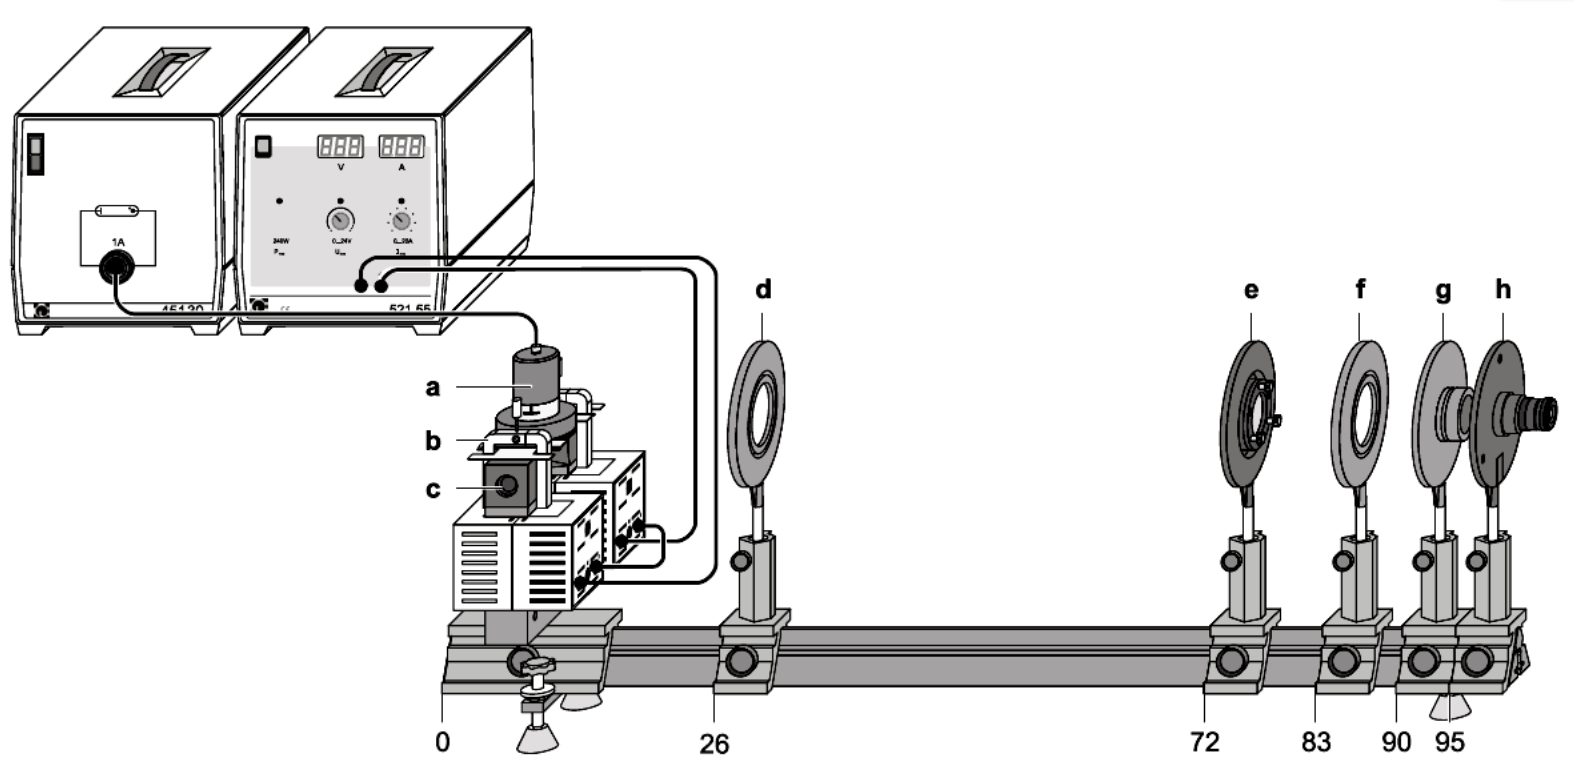
\includegraphics[width=\linewidth]{zeeman-aufbau}
  \caption{Versuchsaufbau Zeeman-Effekt \cite{Leybold}}
  \label{fig:zeeman-aufbau}
\end{figure}
% Der $^1D_2$-Zustand hat Aufspaltungen in $M_J = -2,\,\dots\,,2$ und $^1P_1$ in $M_J=-1,0,1$.
% Es kann also Übergänge mit $\Delta M_J = -1, 0, 1$ geben.
% In Abhängigkeit des $\Delta M$-Werts gibt es verschiedene

Eine Cadmiumlampe (a) ist zwischen den Polschuhen (c) zweier Elektromagneten aufgehängt und wird von einer zugehörigen Stromquelle (oben links) versorgt. 
Im Bild ist die transversale Konfiguration gezeigt, die Magneten mitsamt der Lampe können jedoch gedreht werden,
um auch longitudinal beobachten zu können. Die Magneten werden von einer Hochstromquelle (oben links, rechte Stromquelle) versorgt.
Die Cadmiumlampe beleuchtet eine Kondensorlinse (d). Dadurch, dass die Lampe ausgedehnt ist und in der Brennebene der Linse steht,
gibt es hinter der Linse parallele Lichtbündel mit verschiedenen Winkeln zur optischen Achse.

Diese gehen durch ein Fabry-Perot-Etalon (e), wo der Gangunterschied zwischen parallelen Strahlen von ihrem Einfallswinkel abhängt.
Je nach Winkel eines Lichtbündels findet also entweder konstruktive oder destruktive Interferenz statt.
Dadurch entsteht ein Interferenzmuster von konzentrischen Ringen, welche schließlich durch die Abbildungslinse (f) und das Okular (h)
zur Beobachtung mit dem Auge abgebildet werden.
Die Interferenzbedingung des Interferometers lautet
\begin{equation}
  k\lambda = 2d\sqrt{n^2 - \sin^2(\alpha)}\ \cite{Leybold}\label{eq:fpi-interferenz}
\end{equation}
Der Phasenunterschied hängt nicht nur vom Winkel, sondern auch von der Wellenlänge ab. Betrachtet man leicht unterschiedliche
Wellenlängen, wie hier durch die Zeeman-Aufspaltung, ist also eine Aufspaltung der Ringe zu beobachten.

Um den zu beobachtenden Übergang $^1D_2 \rightarrow\,^1P_1$ herauszufiltern, wird zwischen Abbildungslinse und
Okular ein Farbfilter der Wellenlänge $\lambda=\SI{643.8}{\nm}$ \cite{Anleitung} (g) eingesetzt.


% Folgende wichtige Bestandteile sind zu sehen \cite{Anleitung}:
% \begin{enumerate}[label=\alph*.]
%   \item Cadmium-Lampe
%   \item Klammern
%   \item Polschuhe
%   \item Kondensorlinse
%   \item Polarisationsfilter
%   \item Fabry-Perot-Etalon
%   \item Abbildungslinse
%   \item Interferenzfilter ($\lambda=\SI{643.8}{\nm}$)
%   \item Okular mit Strichskala
% \end{enumerate}
% Außerdem werden Stromquellen (oben links im Bild; links normal, rechts Hochstrom)
% zur Versorgung der Cadmiumlampe und der Elektromagneten eingesetzt.

% Das Fabry-Perot-Etalon in Kombination mit den Linsen erzeugt ein Interferenzmuster mit Ringen,
% deren Position von der Wellenlänge des Lichts abhängt.
% Der Interferenzfilter wird eingesetzt, um ausschließlich das Licht vom Übergang $^1D_2 \rightarrow\,^1P_1$ betrachten zu können.

Zur Justage des Aufbaus wird am Okular die Strichskala scharfgestellt und
die Abbildungslinse verschoben, bis das Interferenzmuster der Lampe durch das Etalon scharf zu sehen ist.
Das Etalon wird so gedreht, dass das Zentrum des Musters am Nullpunkt der Strichskala ist
und die Kondensorlinse verschoben, um eine gleichmäßige Ausleuchtung zu erhalten.

\subsection{Beobachtung des Zeeman-Effekts}
\subsubsection{transversale Konfiguration}
Zunächst wird in transversaler Konfiguration ohne eingesetzten Polarisationsfilter beobachtet,
d.h. die optische Achse steht senkrecht zum Magnetfeld, wie in Abb. \ref{fig:zeeman-aufbau} gezeigt.
Nach Abb. \ref{fig:zeeman-abstrahlung} sollte hier sowohl Strahlung vom $\pi$-Übergang,
als auch den $\sigma^\pm$-Übergängen, zu sehen sein.
Hierbei ist die Strahlung der beiden verschiedenen $\sigma$-Übergänge gleich polarisiert;
die Polarisation vom $\pi$-Übergang steht senkrecht dazu.

\begin{figure}[H]
  \centering
  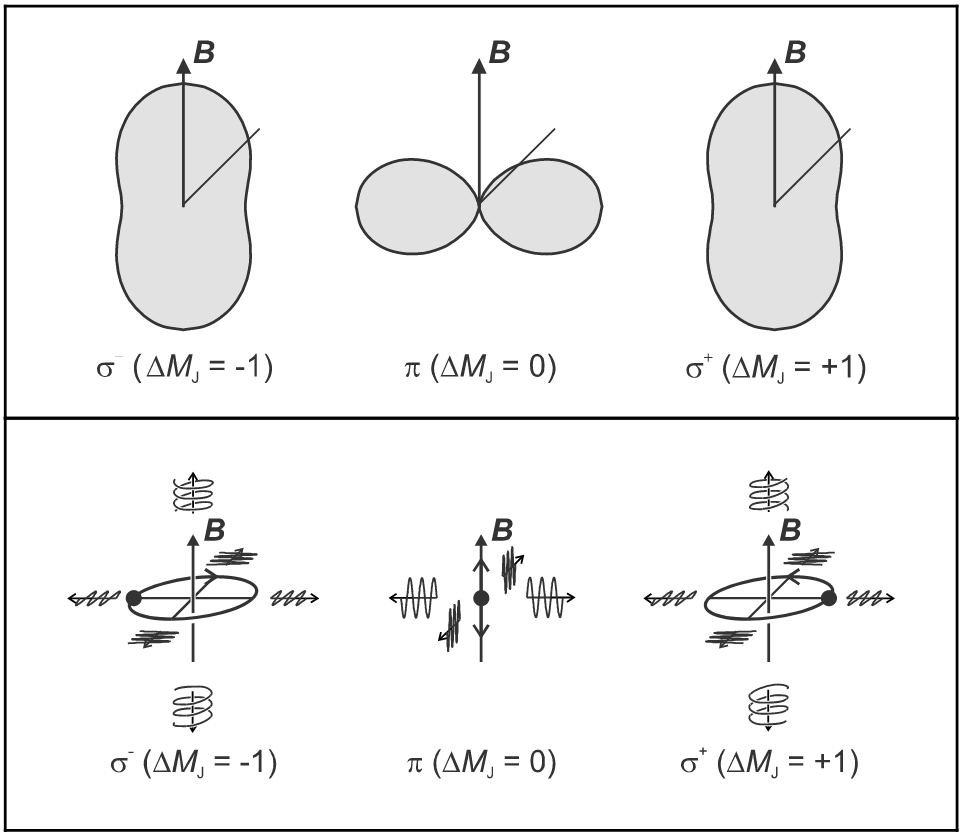
\includegraphics[width=.8\linewidth]{zeeman-abstrahlung}
  \caption{Polarisationsverteilung und Abstrahlungscharakteristik elektrischer Dipolübergänge \cite{Anleitung} \cite{Leybold}.}
  \label{fig:zeeman-abstrahlung}
\end{figure}

Das am Okular enstehende Bild ist in Abb. \ref{fig:zeeman-transveral-ohne-ohne} gezeigt.
\begin{figure}[H]
  \centering
  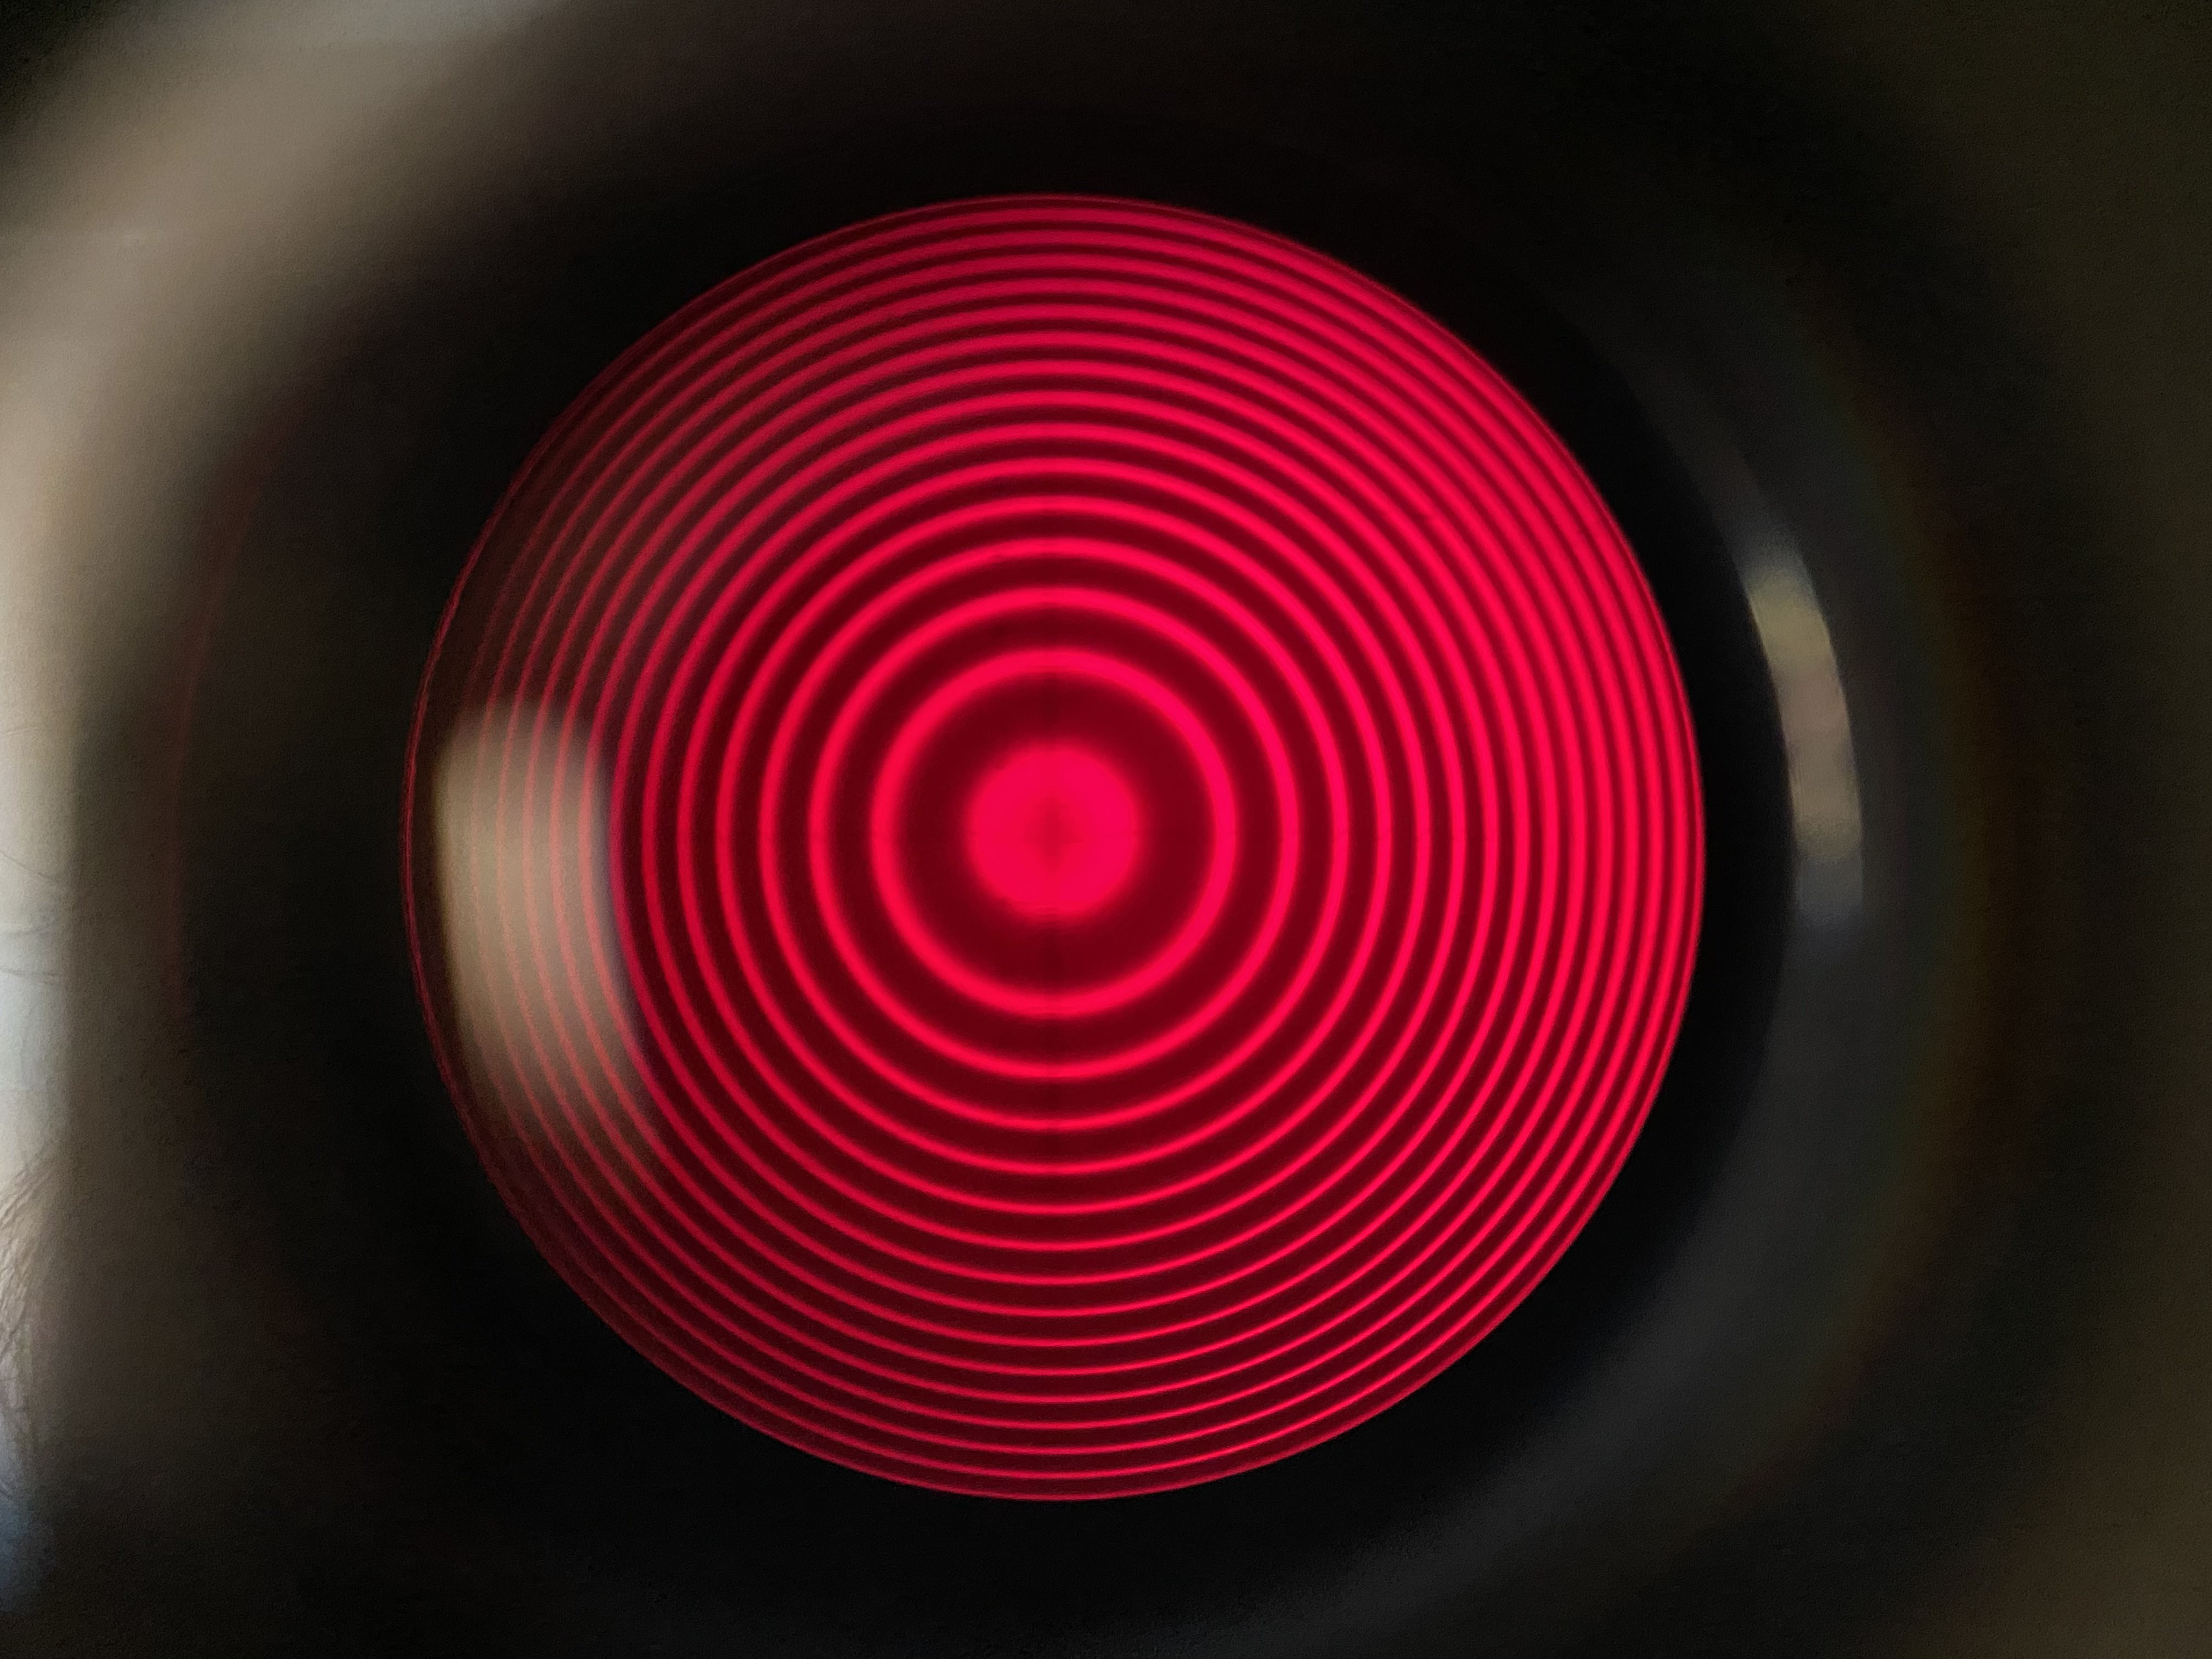
\includegraphics[width=.8\linewidth]{zeeman-transversal-ohne-ohne}
  \caption{Interferenzmuster bei transversaler Beobachtung ohne Magnetfeld, ohne Polarisationsfilter.}
  \label{fig:zeeman-transveral-ohne-ohne}
\end{figure}
Es sind die verschiedenen Interferenzringe zu erkennen, die hier alle von der gleichen Wellenlänge stammen.

Nun wird das Magnetfeld eingeschaltet und erhöht, bis man eine Aufspaltung der einzelnen Ringe sieht, siehe Abb. \ref{fig:zeeman-transveral-mit-ohne}
\begin{figure}[H]
  \centering
  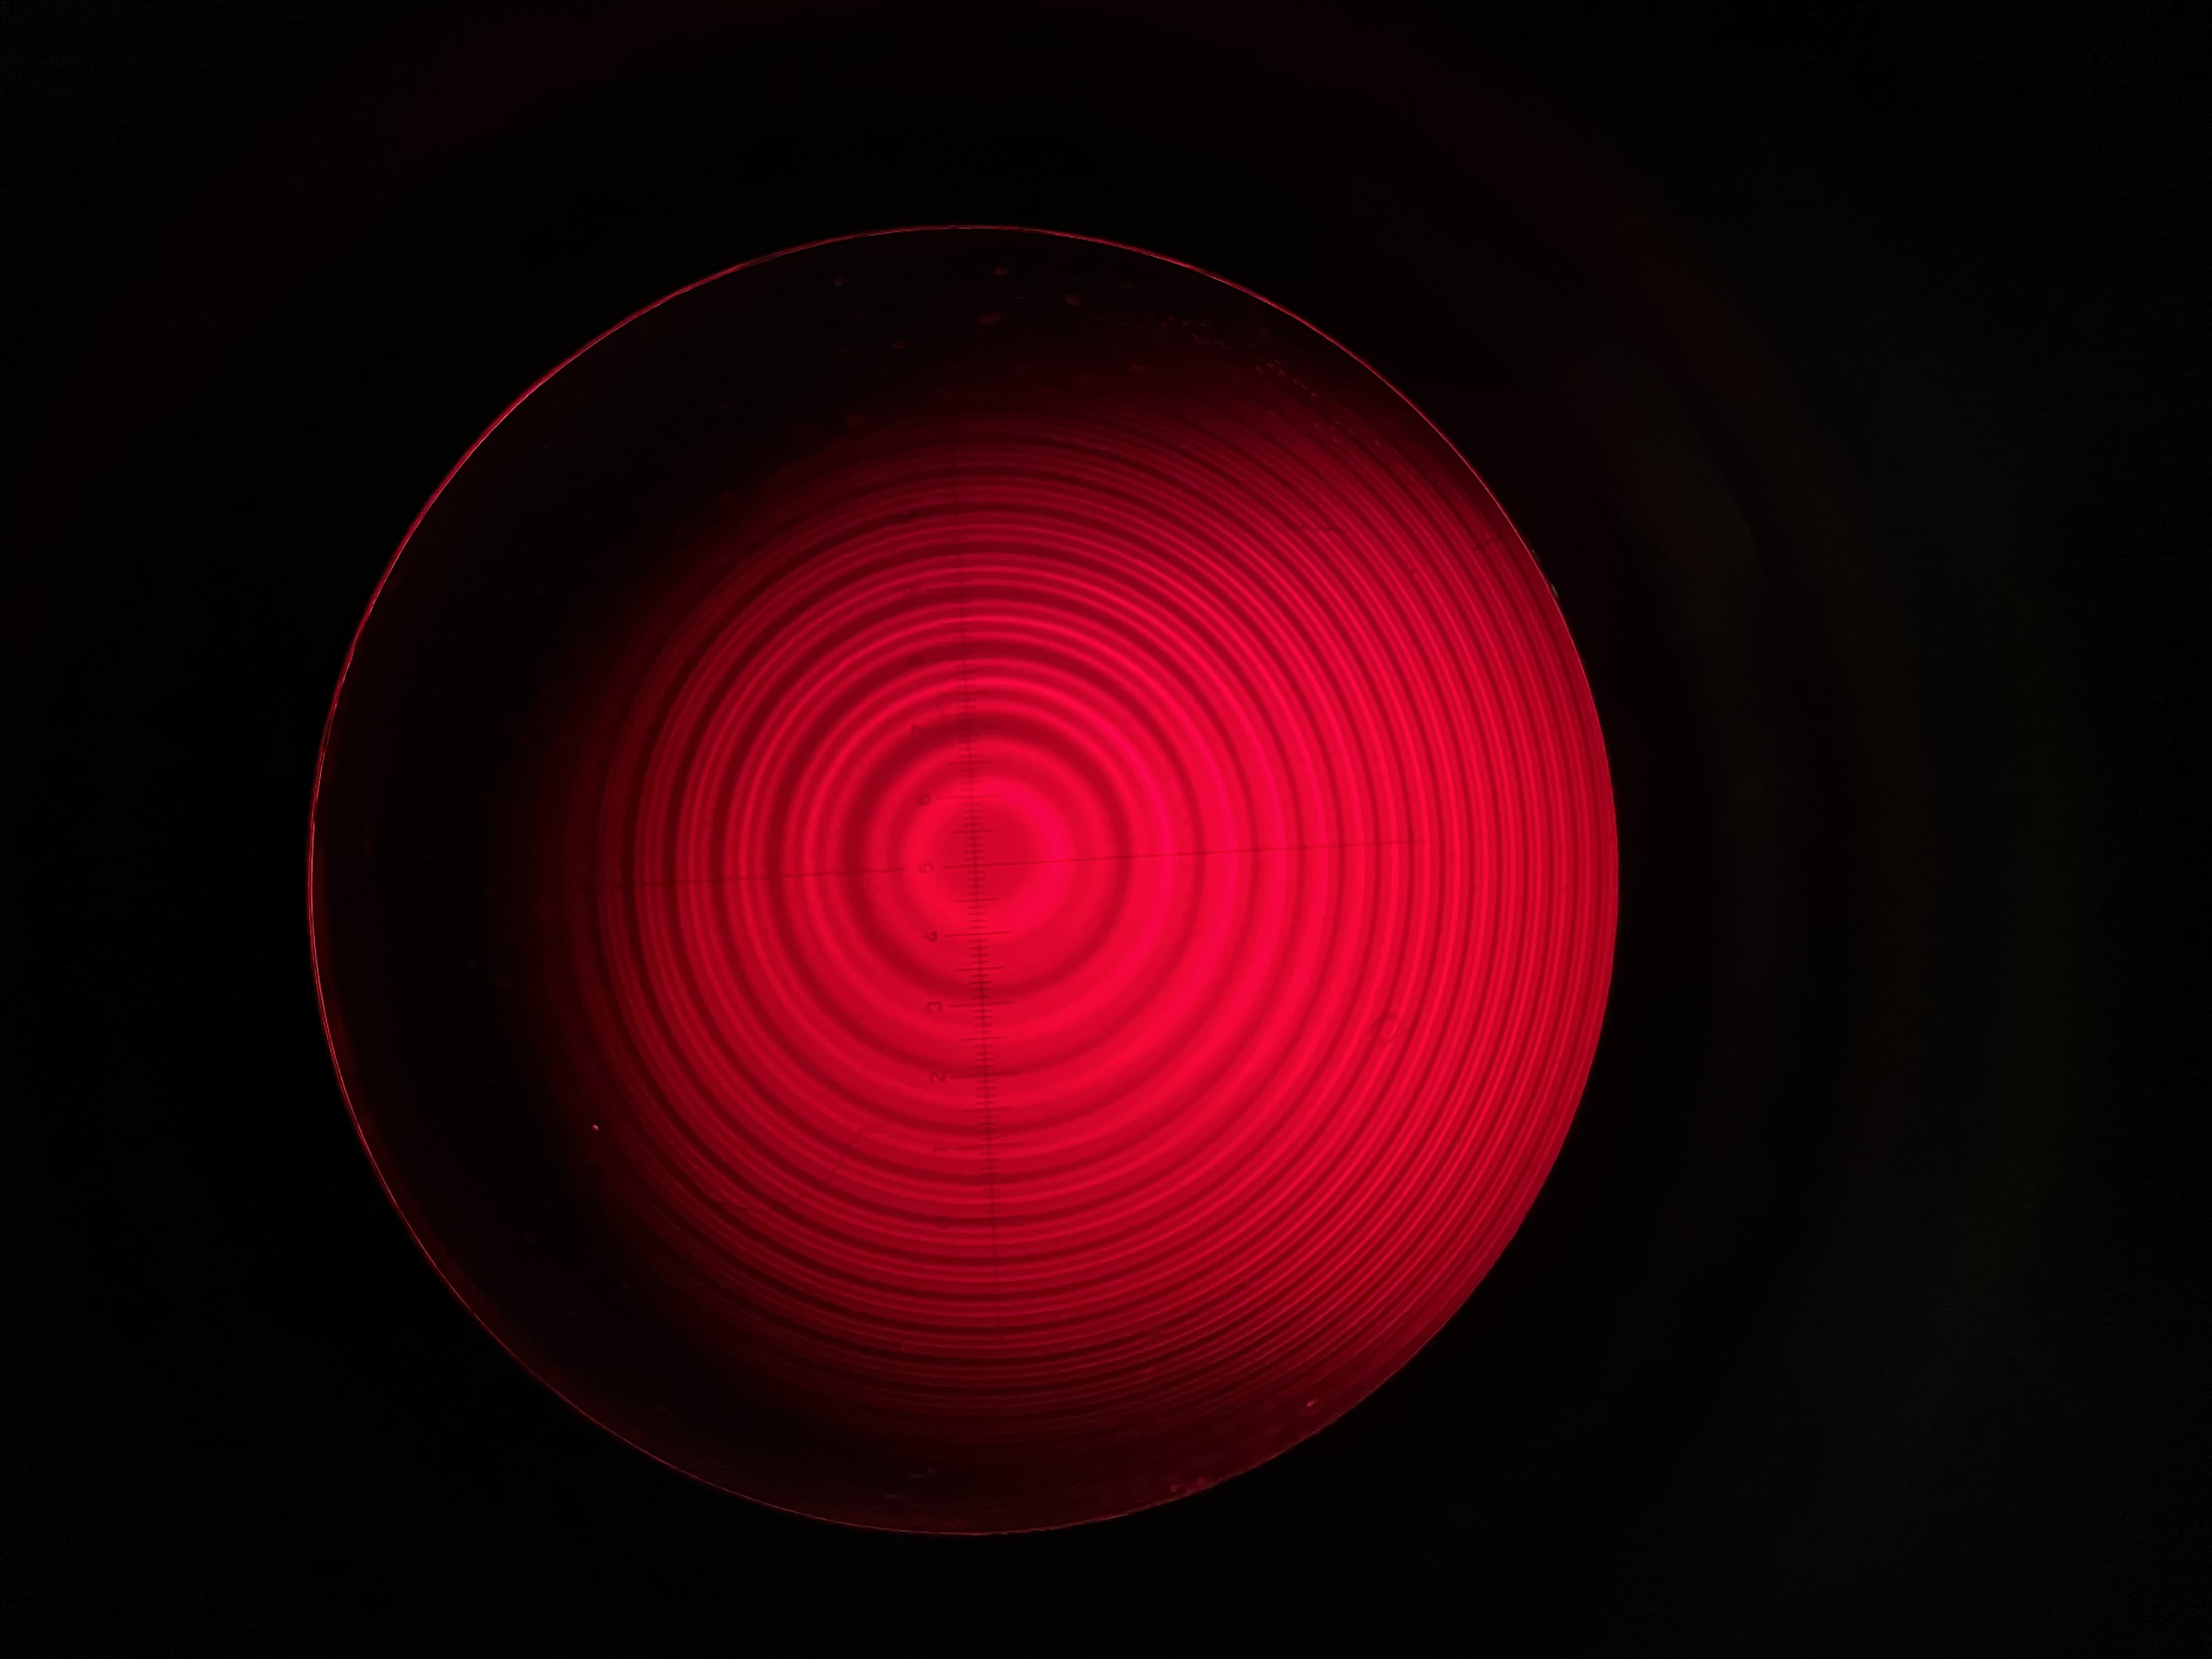
\includegraphics[width=.8\linewidth]{zeeman-transversal-mit-ohne}
  \caption{Interferenzmuster bei transversaler Beobachtung mit Magnetfeld, ohne Polarisationsfilter.}
  \label{fig:zeeman-transveral-mit-ohne}
\end{figure}
Die Aufspaltung der Ringe lässt sich durch den Zeeman-Effekt erklären. Der $\pi$-Übergang mit $\Delta m_J=0$ ist nach \eqref{eq:delta-e}
unbeeinflusst, während die $\sigma$-Übergänge eine Änderung ihrer Energie proportional zu $B$ erfahren.
Was zuvor ein Ring war, spaltet sich daher in drei Ringe leicht unterschiedlicher Wellenlängen auf.

Die verschiedenen Komponenten können durch Einsatz eines Polarisationsfilters zwischen Kondensorlinse und Etalon
herausgefiltert werden (Abb. \ref{fig:zeeman-transveral-mit-90}, \ref{fig:zeeman-transveral-mit-0}).
\begin{figure}[H]
  \centering
  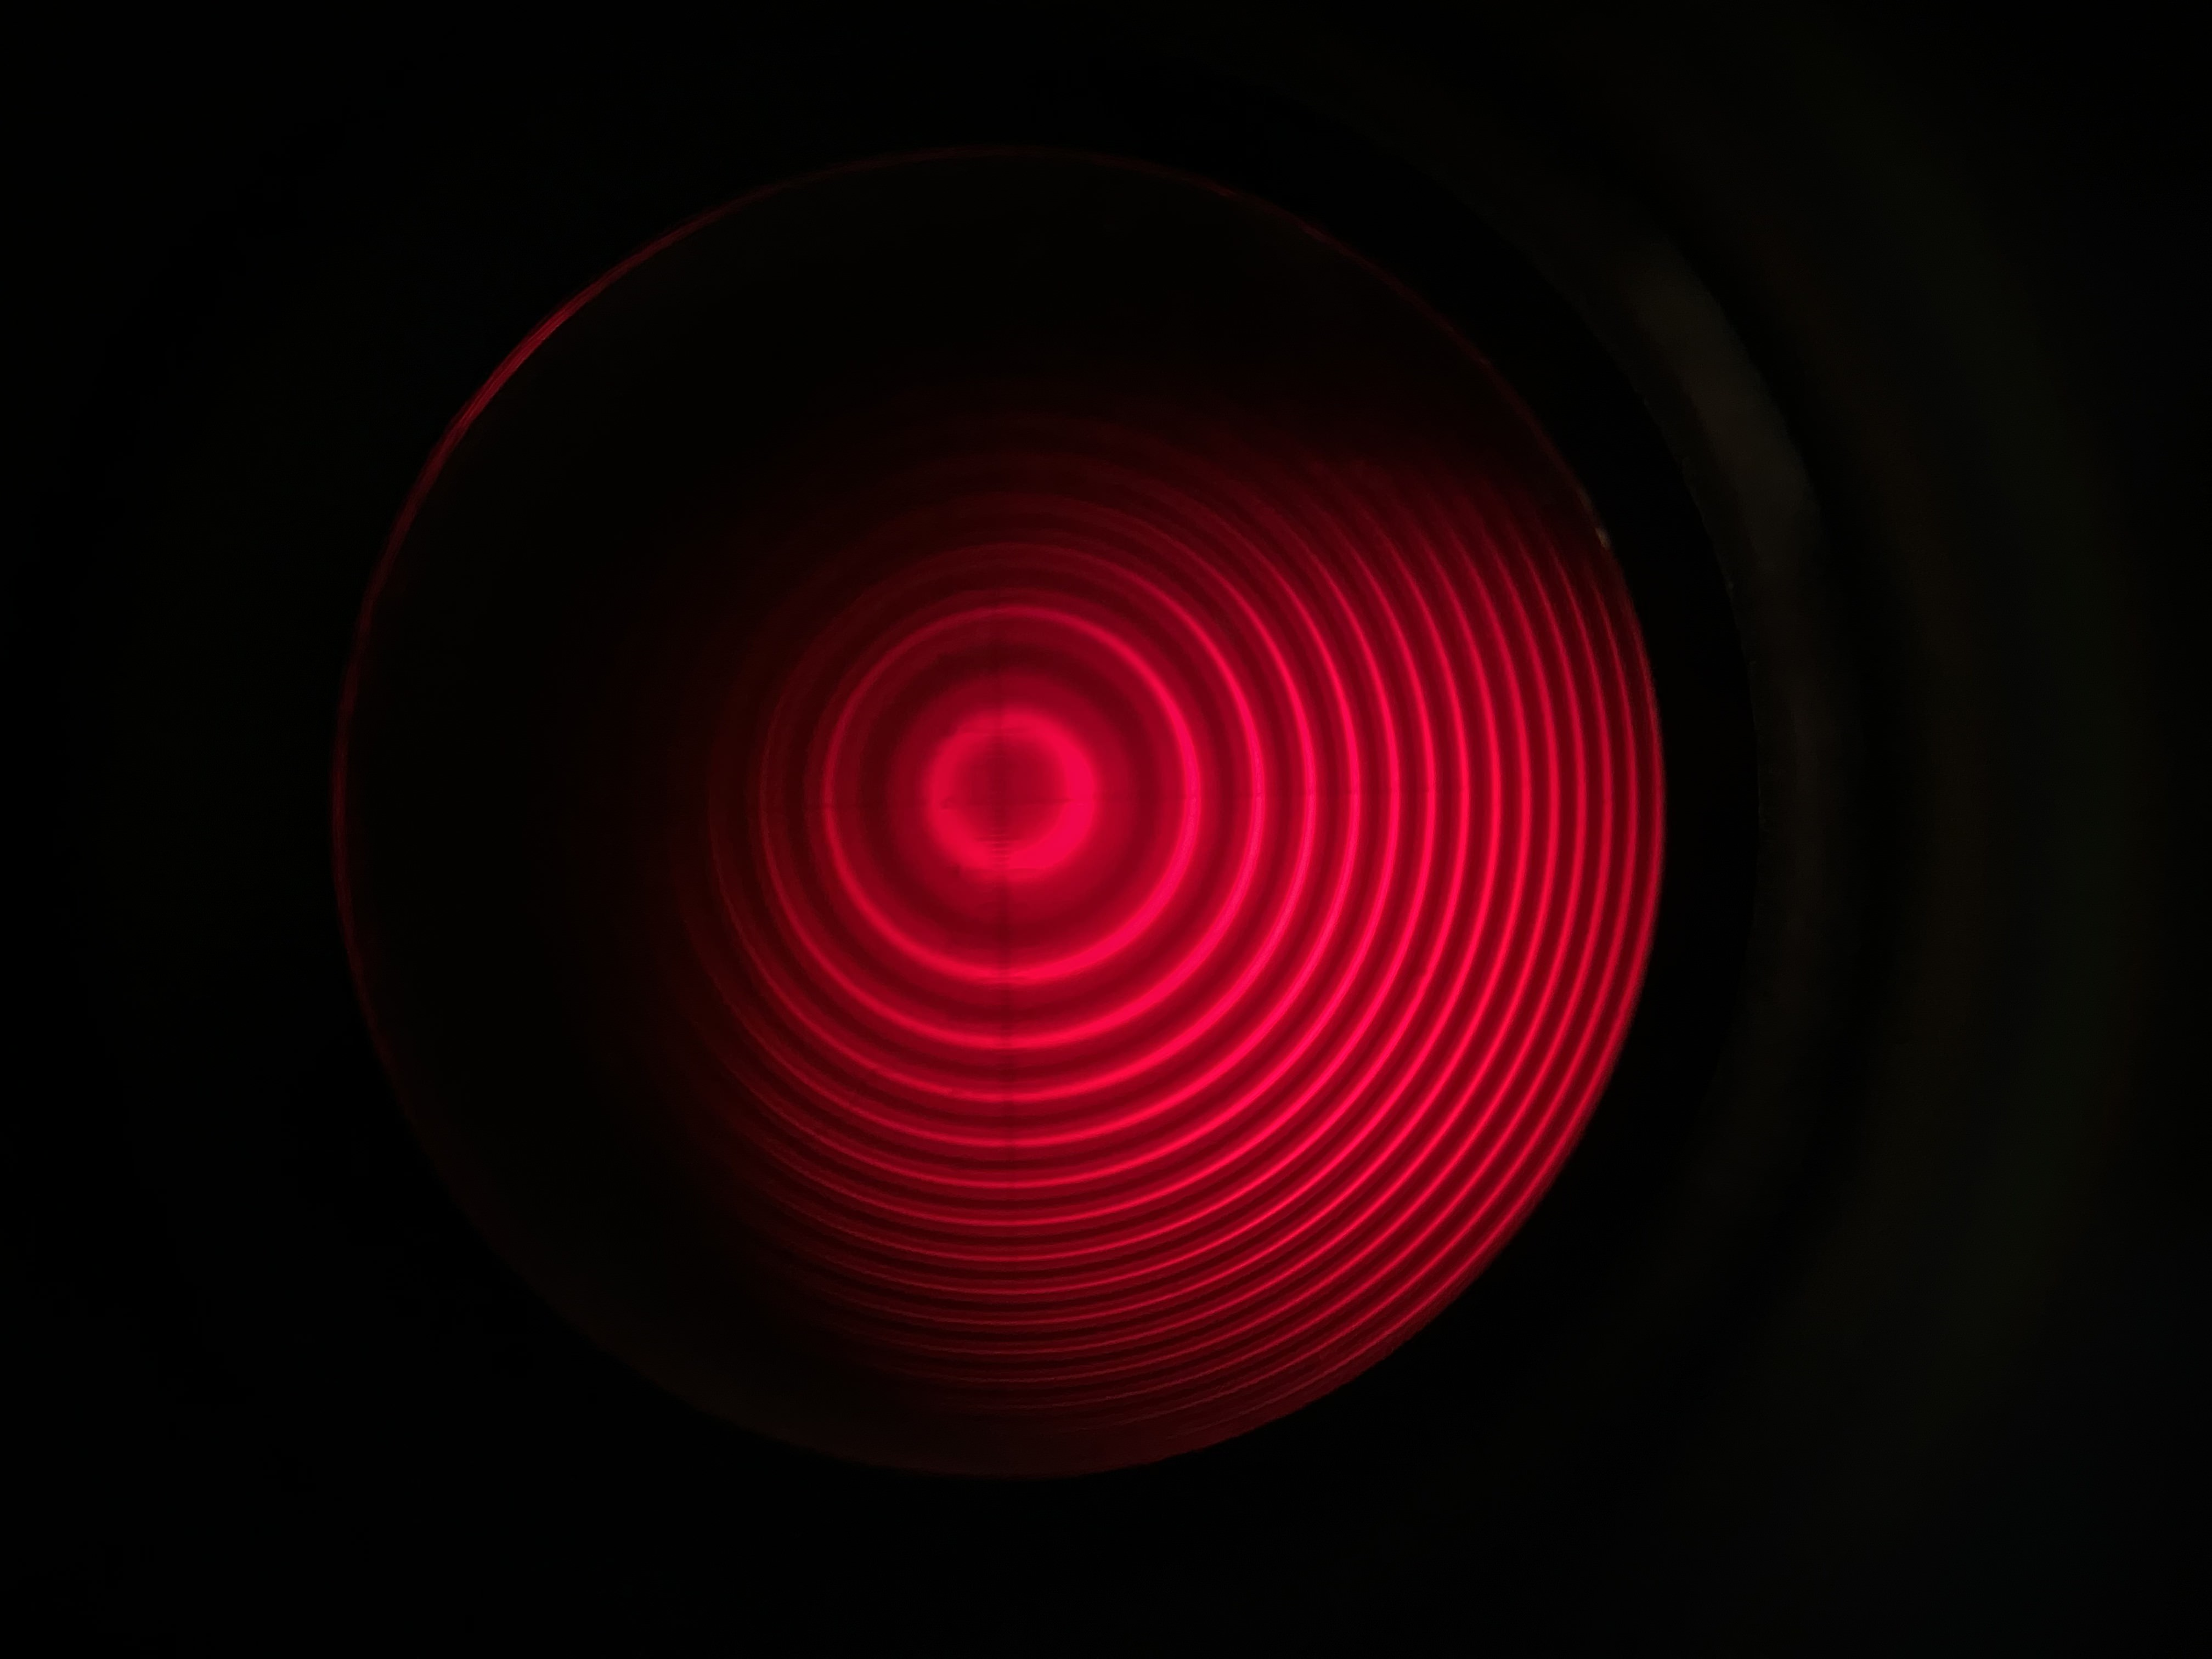
\includegraphics[width=.8\linewidth]{zeeman-transversal-mit-90}
  \caption{Interferenzmuster bei transversaler Beobachtung mit Magnetfeld, mit Polarisationsfilter auf \ang{90}.}
  \label{fig:zeeman-transveral-mit-90}
\end{figure}
\begin{figure}[H]
  \centering
  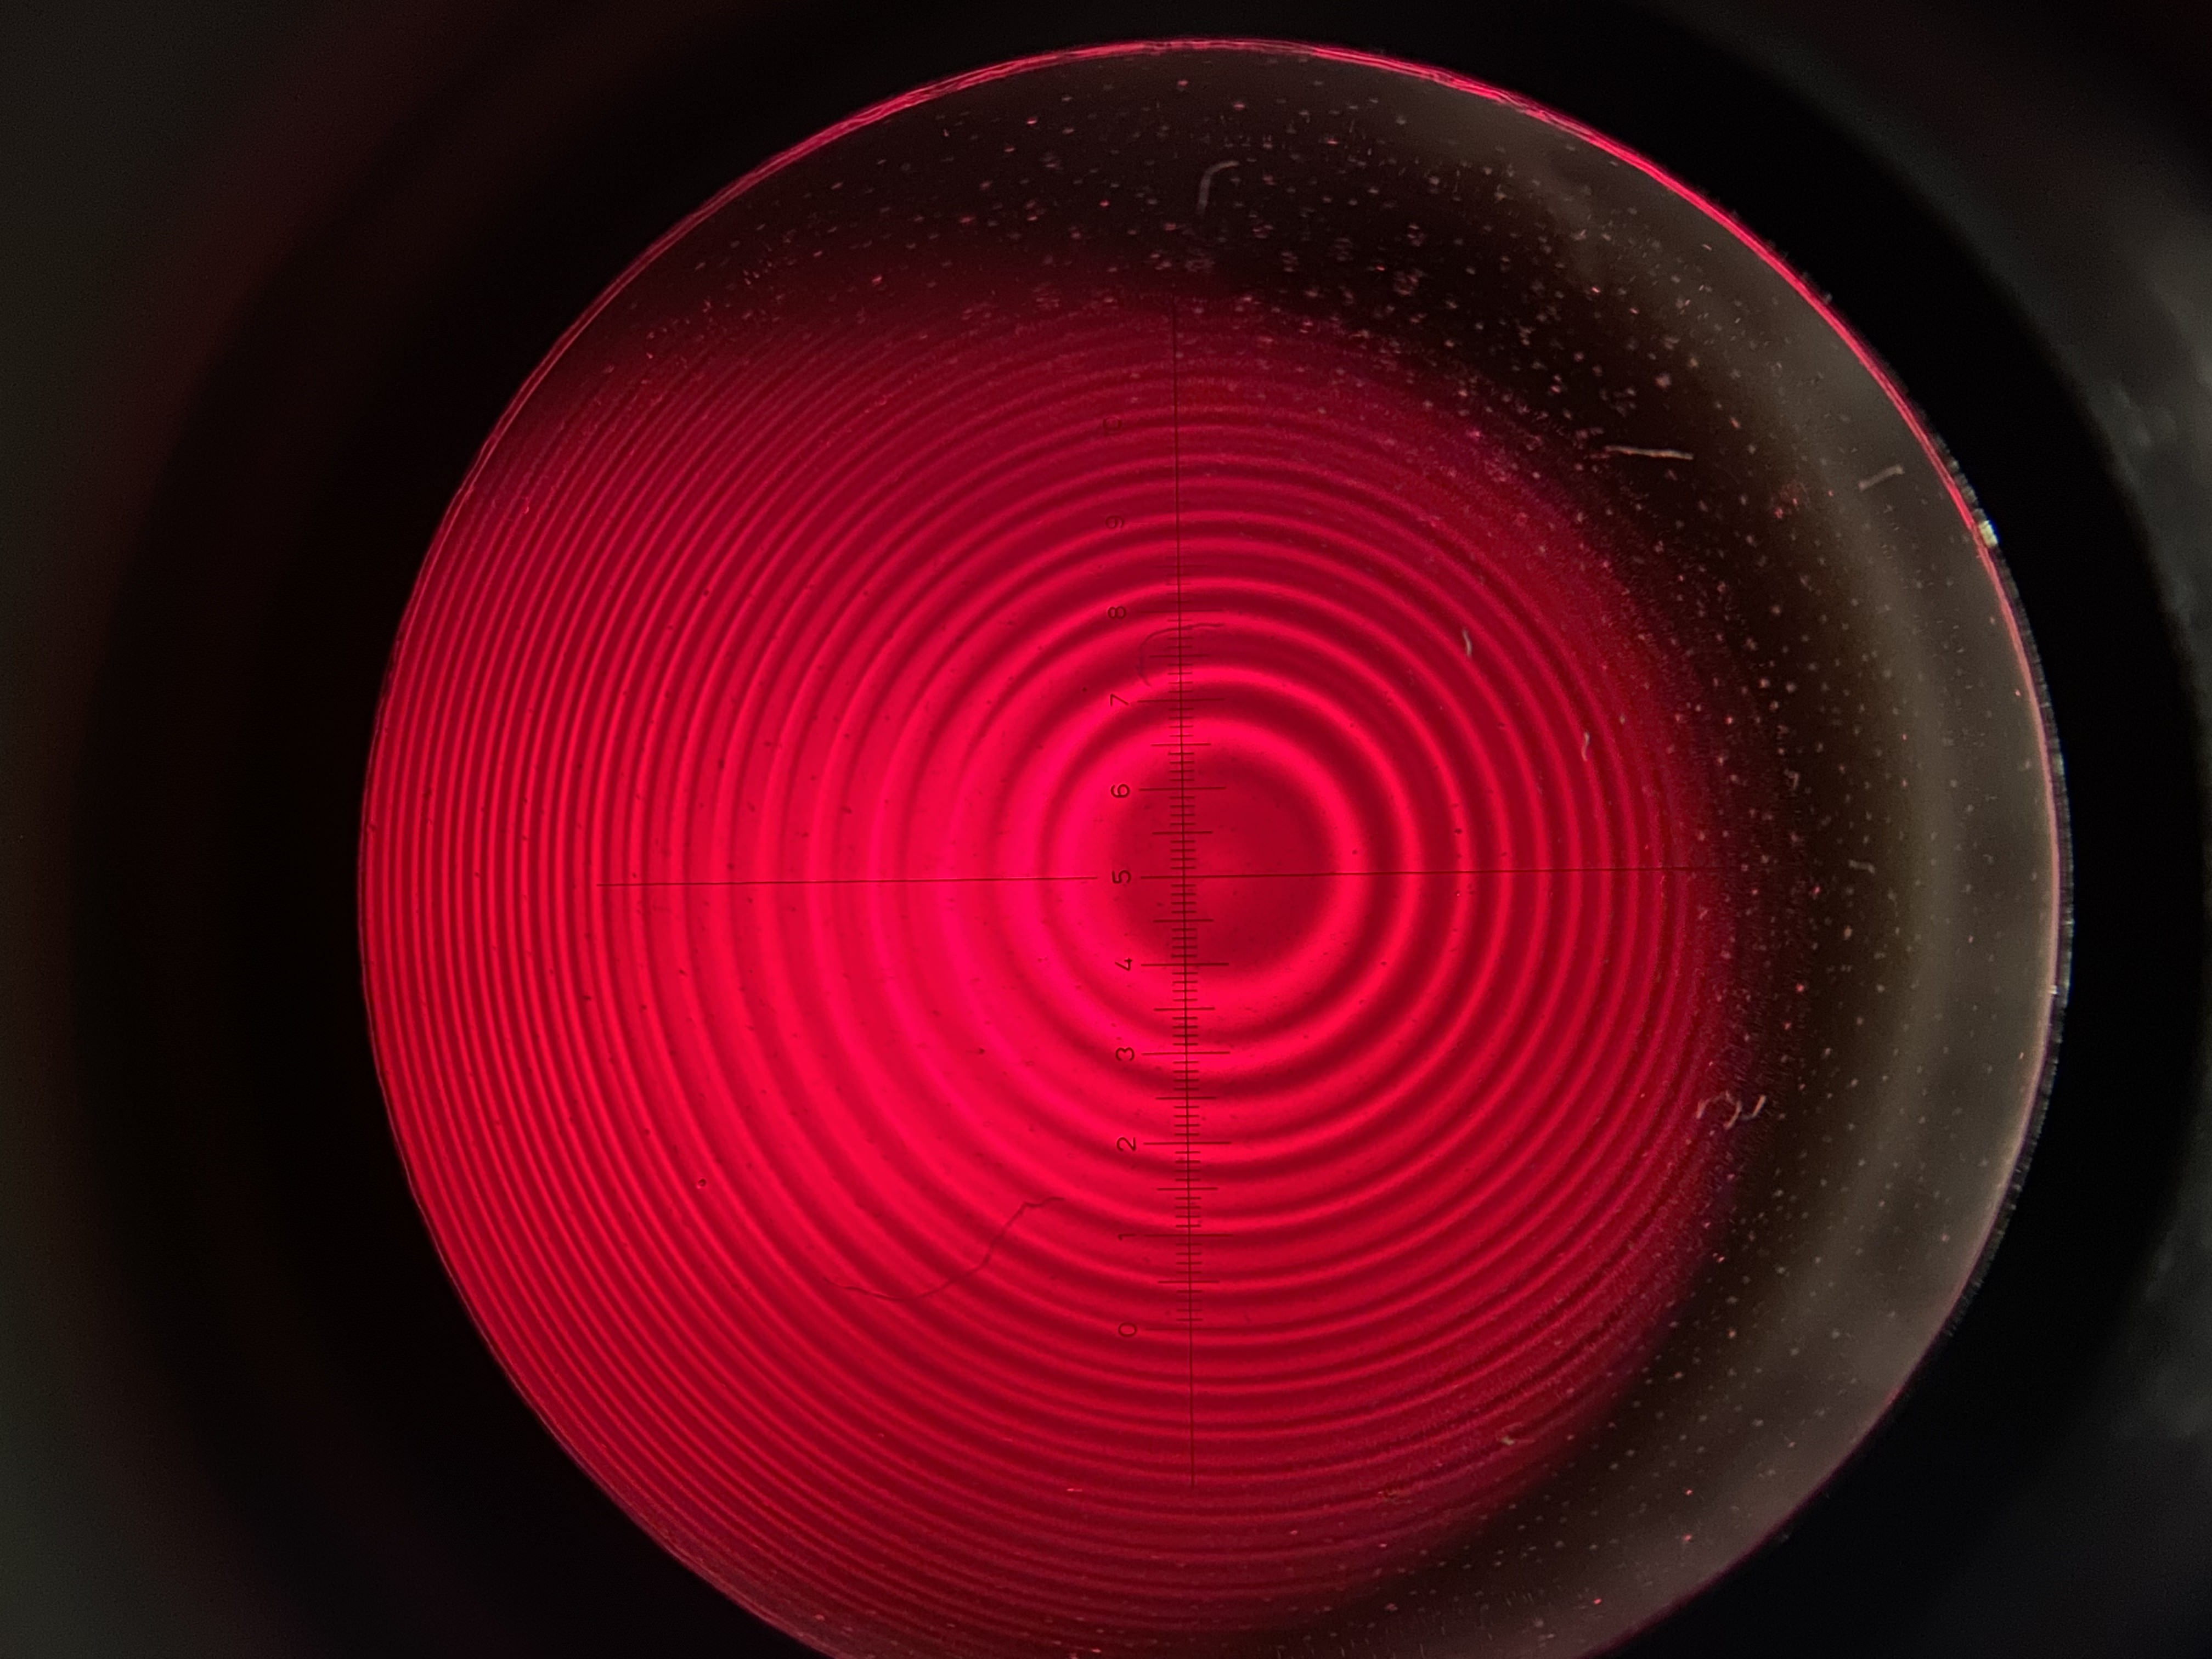
\includegraphics[width=.8\linewidth]{zeeman-transversal-mit-0}
  \caption{Interferenzmuster bei transversaler Beobachtung mit Magnetfeld, mit Polarisationsfilter auf \ang{0}.}
  \label{fig:zeeman-transveral-mit-0}
\end{figure}
Wenn der Filter auf \ang{90} steht, sind wieder nur einzelne Ringe zu sehen, die dem $\pi$-Übergang entsprechen,
welcher Licht mit Polarisation parallel zum Magnetfeld produziert.
Steht der Filter auf \ang{0}, gibt es jeweils zwei Ringe, die $\sigma^+$ bzw. $\sigma^-$ entsprechen.


\subsubsection{longitudinale Konfiguration}
Die Magneten mitsamt der Cadmiumlampe werden um \ang{90} gedreht,
um die Beobachtungen in longitudinaler Konfiguration (Magnetfeld parallel zur optischen Achse bzw. der Beobachtungsrichtung)
zu wiederholen.

Ohne Magnetfeld ergibt sich das Muster in Abb. \ref{fig:zeeman-longitudinal-ohne-ohne}, was mit der entsprechenden Beobachtung
bei transversaler Konfiguration übereinstimmt. Da kein Magnetfeld anliegt, können $\pi$ und $\sigma^\pm$-Übergänge nicht unterschieden
werden alle Betrachtungsrichtungen lassen das gleiche Muster erkennen.
\begin{figure}[H]
  \centering
  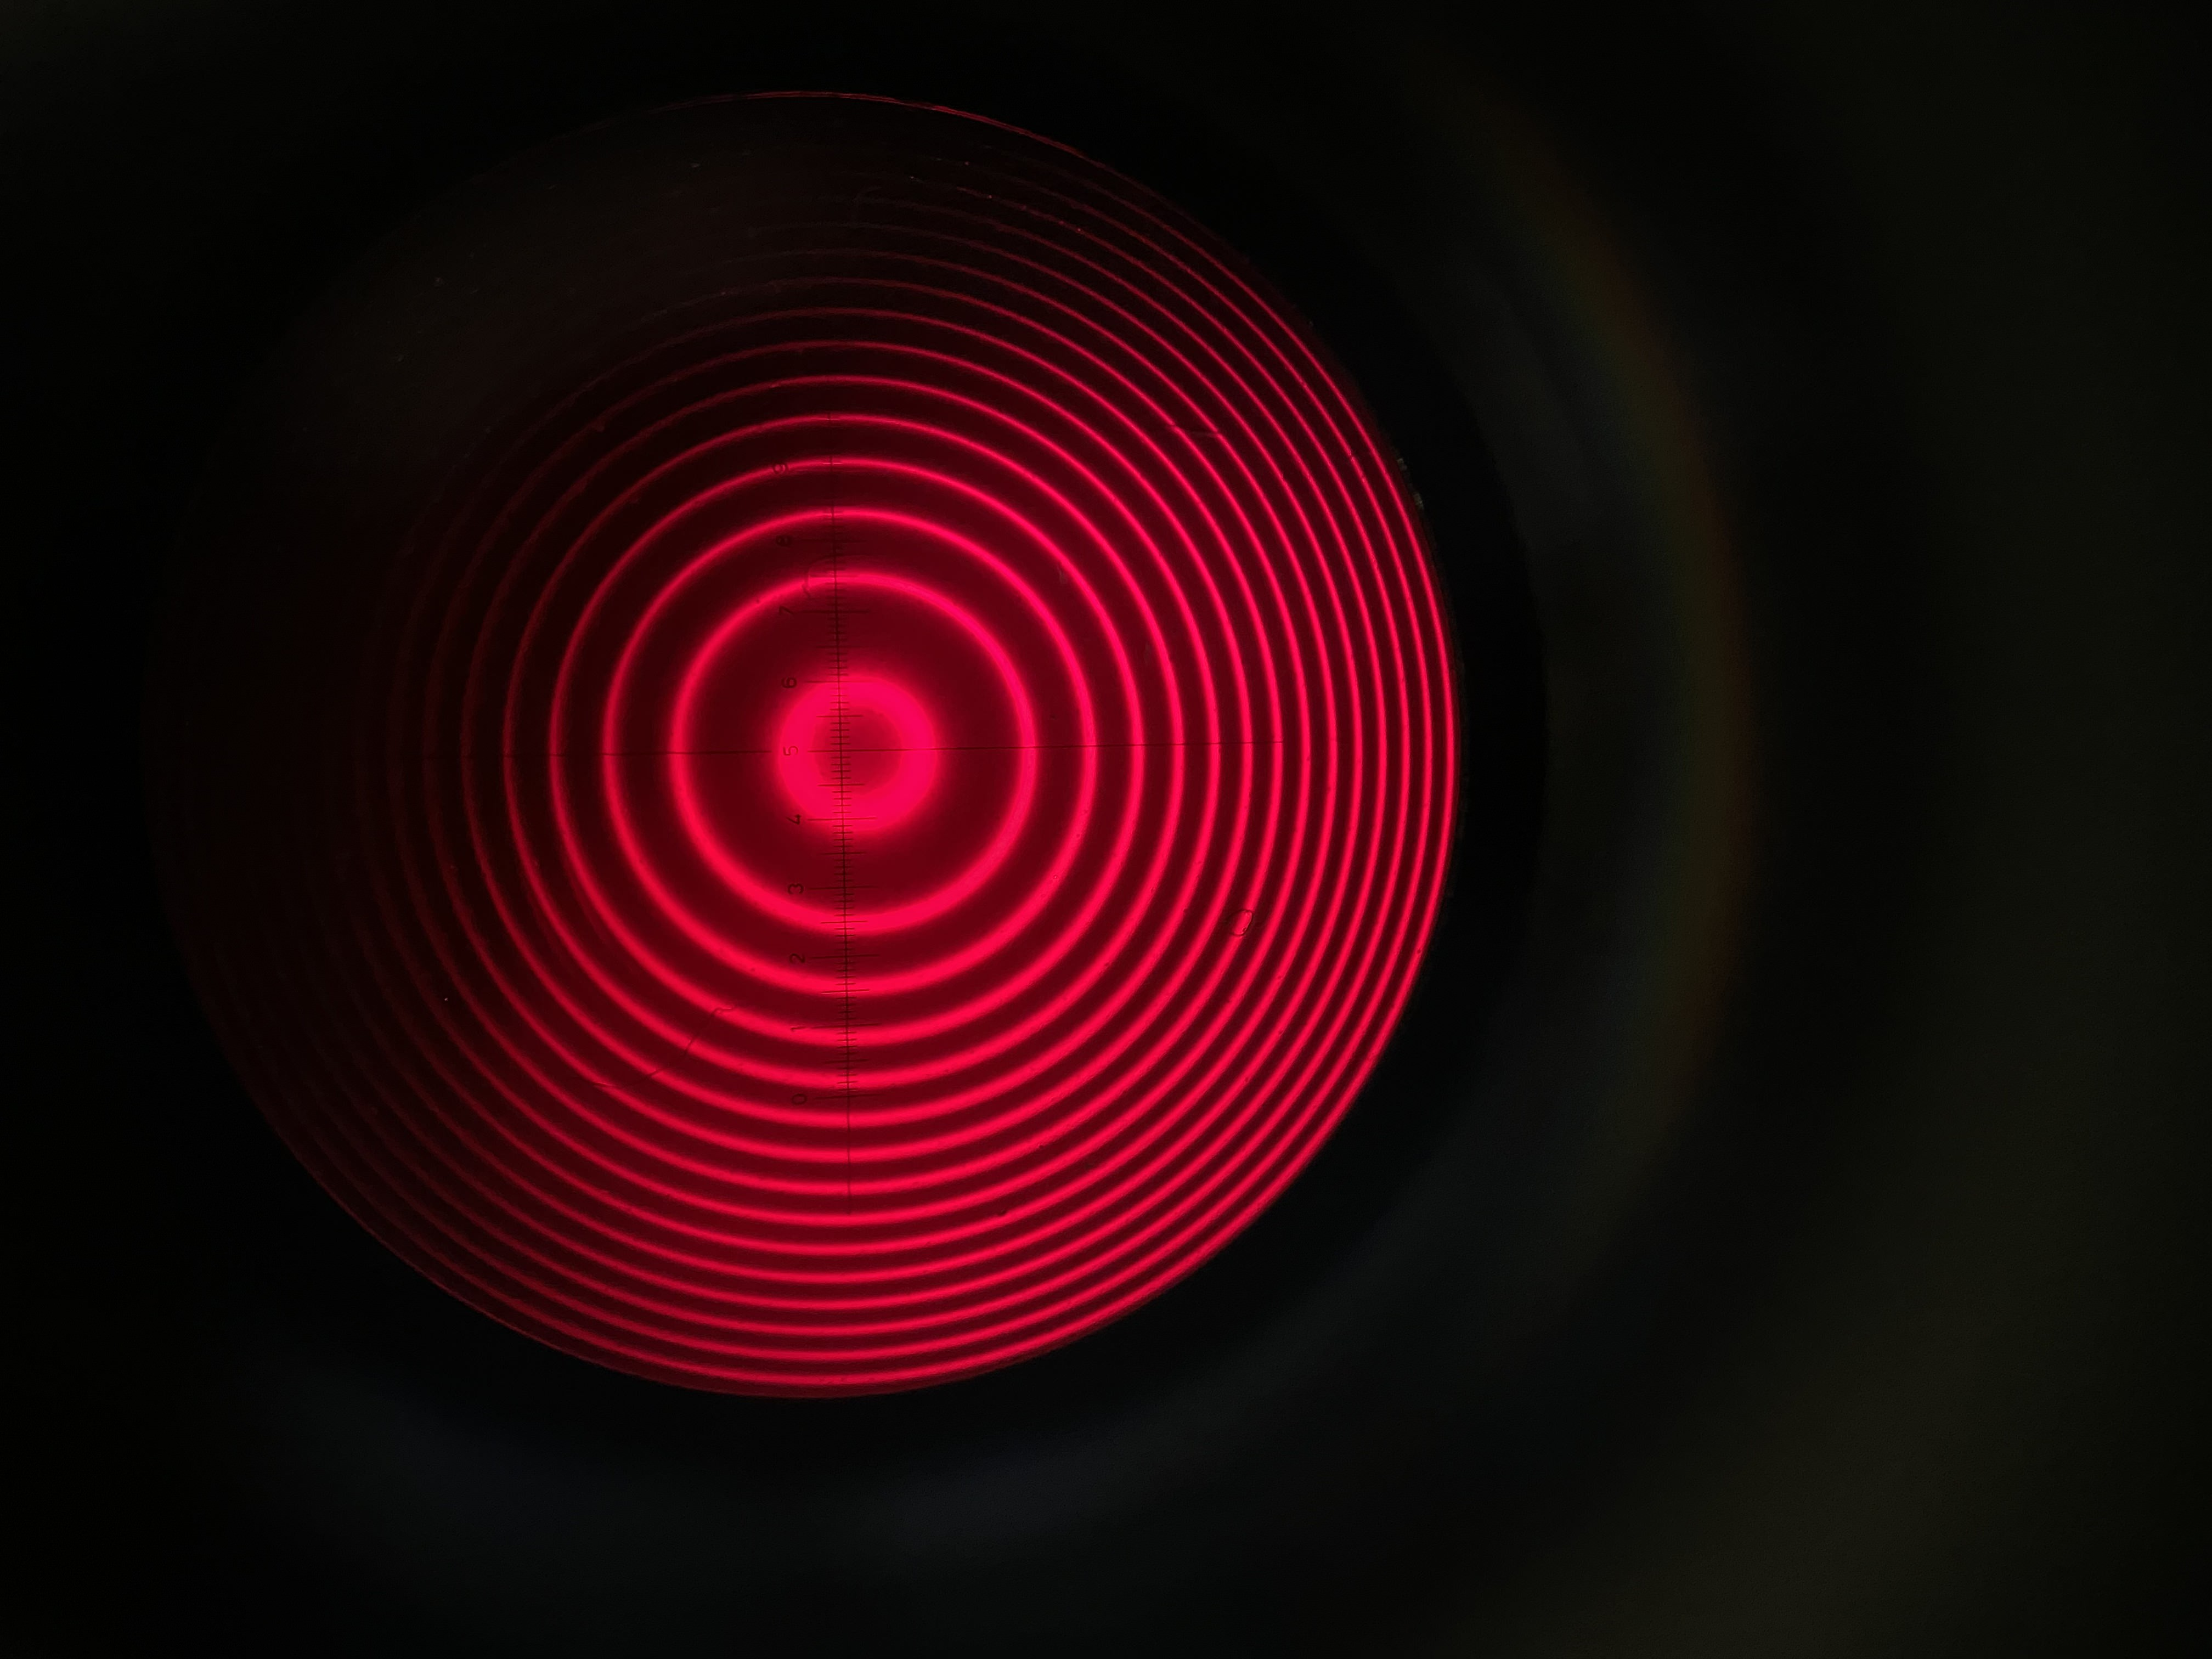
\includegraphics[width=.8\linewidth]{zeeman-longitudinal-ohne-ohne}
  \caption{Interferenzmuster bei longitudinaler Beobachtung ohne Magnetfeld, ohne Polarisationsfilter.}
  \label{fig:zeeman-longitudinal-ohne-ohne}
\end{figure}

Wird das Magnetfeld angeschaltet (Abb. \ref{fig:zeeman-longitudinal-mit-ohne}),
ist eine Aufspaltung eines Rings in jeweils zwei Ringe zu beobachten.
Diese entsprechen den beiden $\sigma$-Übergängen, während der $\pi$-Übergang aufgrund seiner Abstrahlungscharakteristik
in longitudinaler Konfiguration nicht zu sehen ist.
\begin{figure}[H]
  \centering
  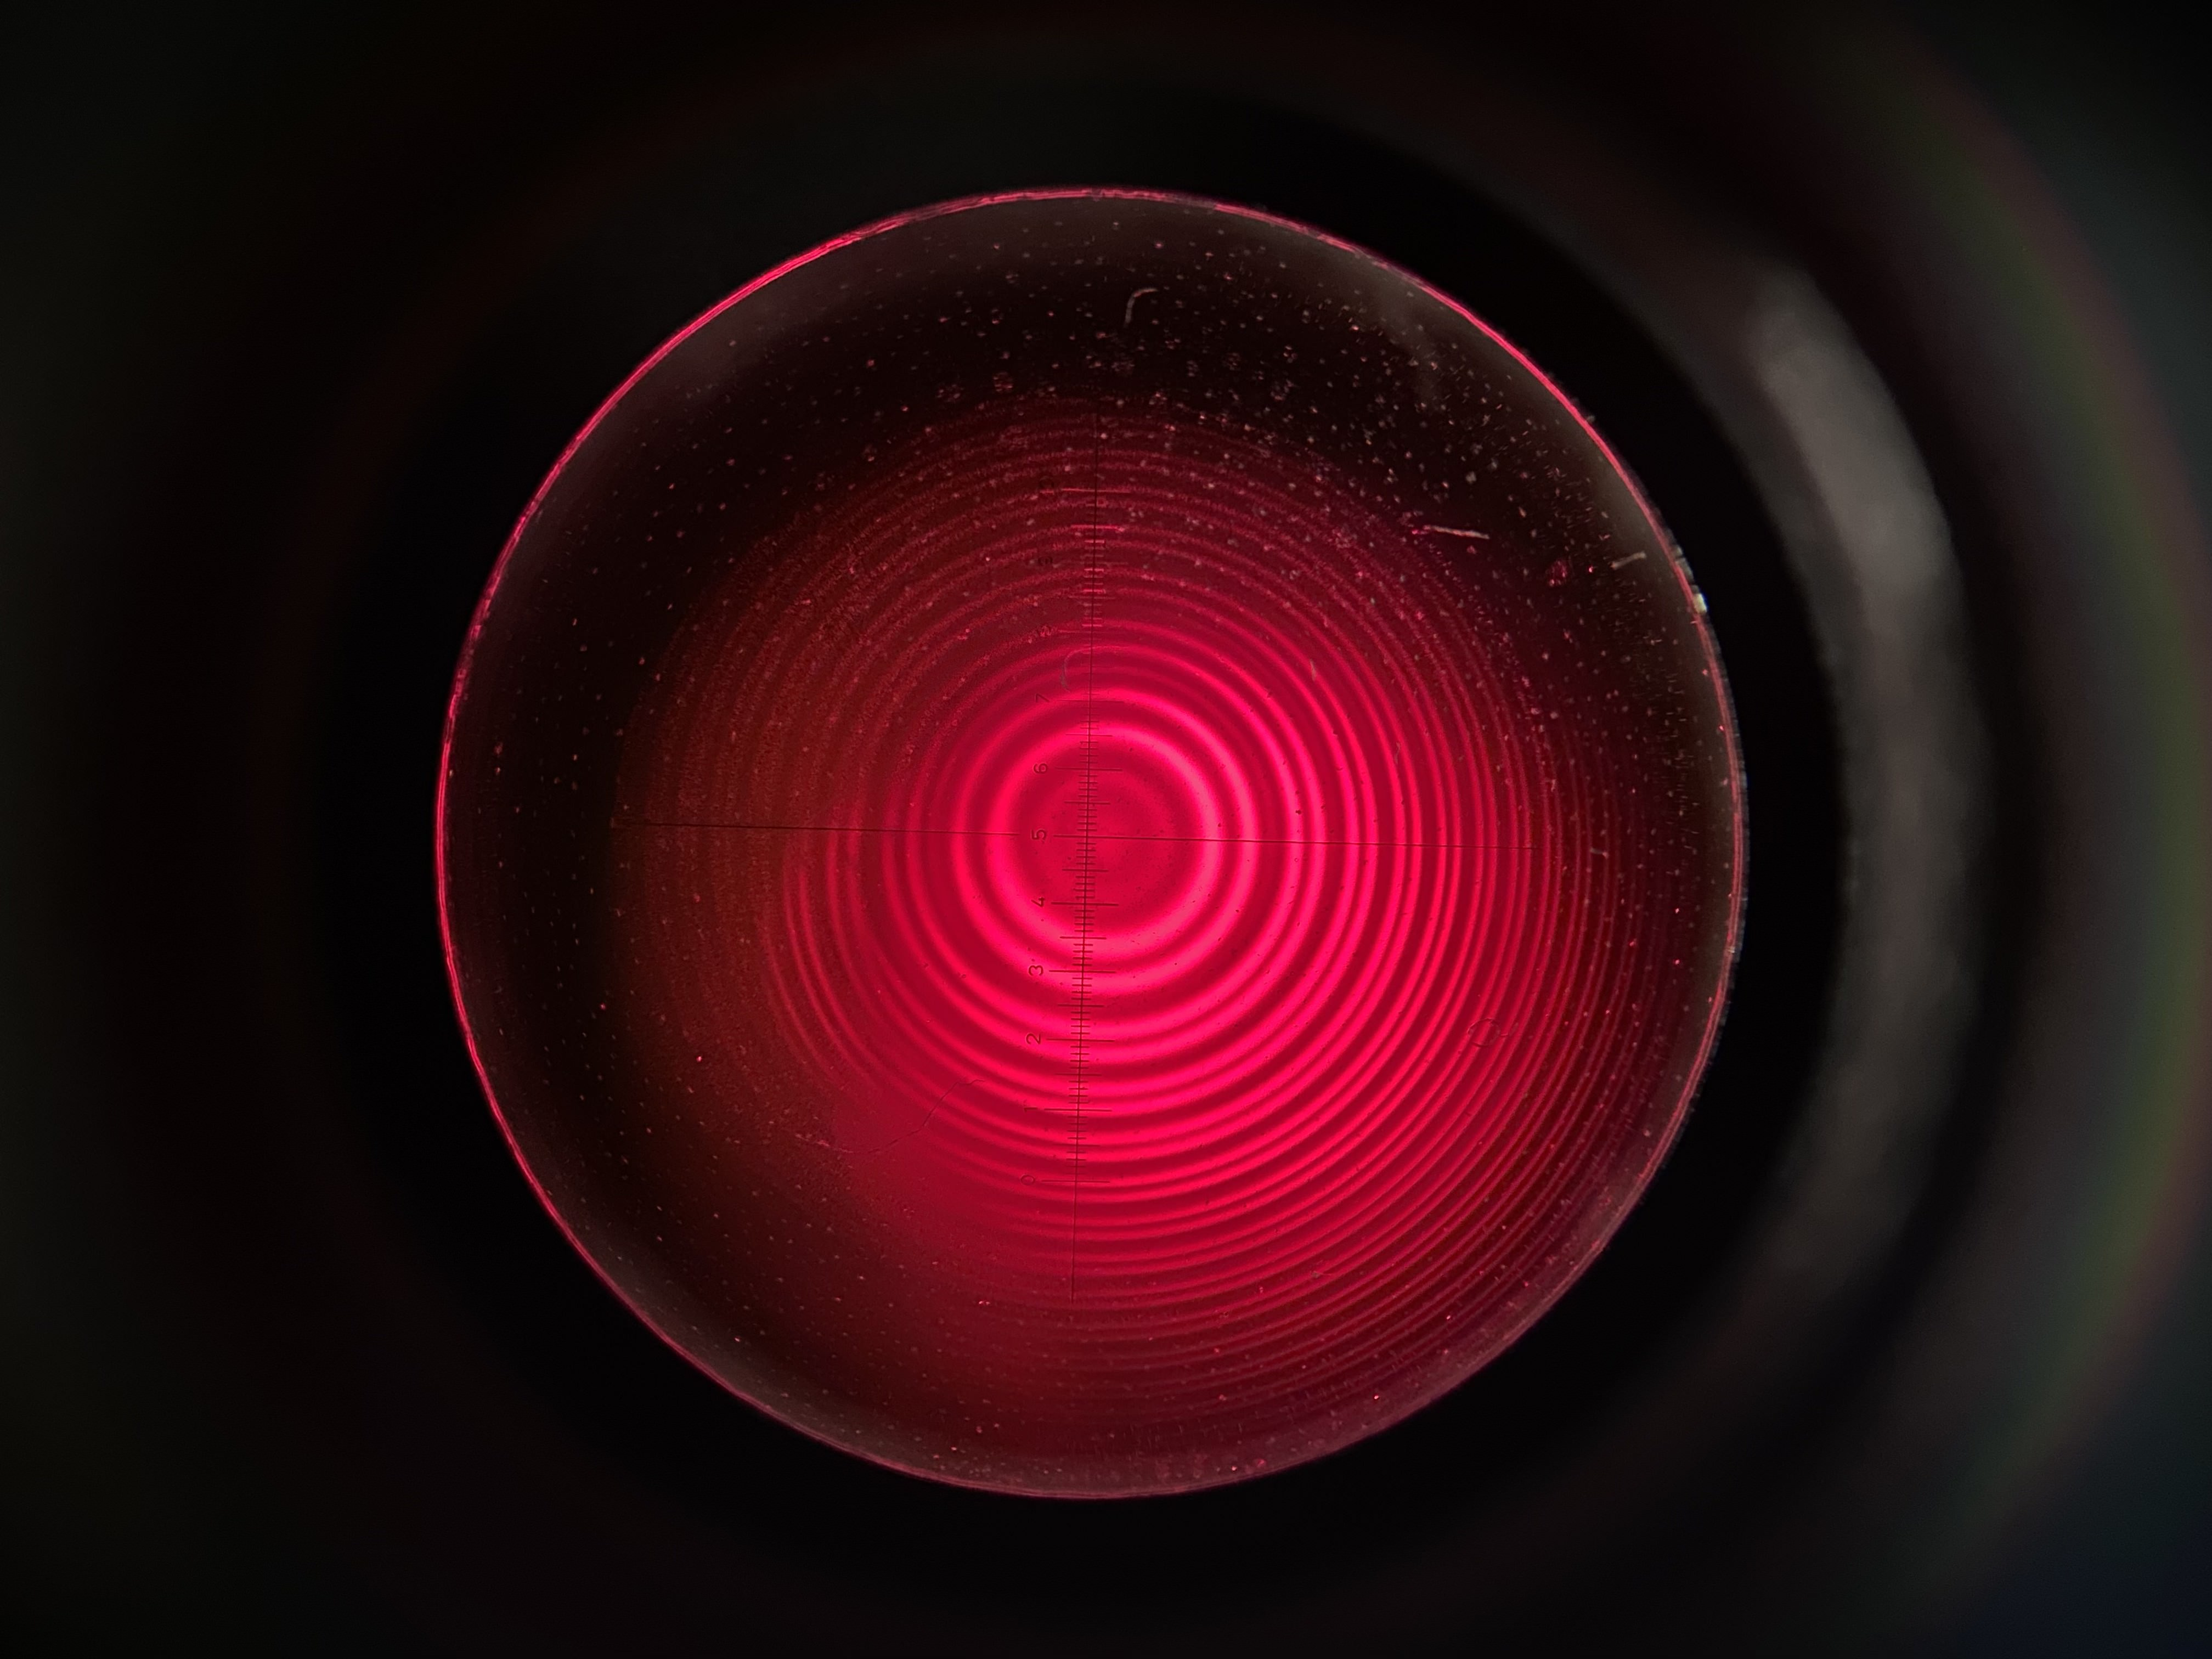
\includegraphics[width=.8\linewidth]{zeeman-longitudinal-mit-ohne}
  \caption{Interferenzmuster bei longitudinaler Beobachtung mit Magnetfeld, ohne Polarisationsfilter.}
  \label{fig:zeeman-longitudinal-mit-ohne}
\end{figure}

Als nächstes wird zusätzlich eine $\lambda / 4$-Platte in \ang{0}-Stellung in den Strahlengang vor dem
Polarisationsfilter eingesetzt. 

Mit dem Polarisationsfilter auf \ang{-45} ist in jeder Beugungsordnung statt zwei Ringen nur noch ein Ring stark zu sehen (Abb. \ref{fig:zeeman-longitudinal-mit--45})
\begin{figure}[H]
  \centering
  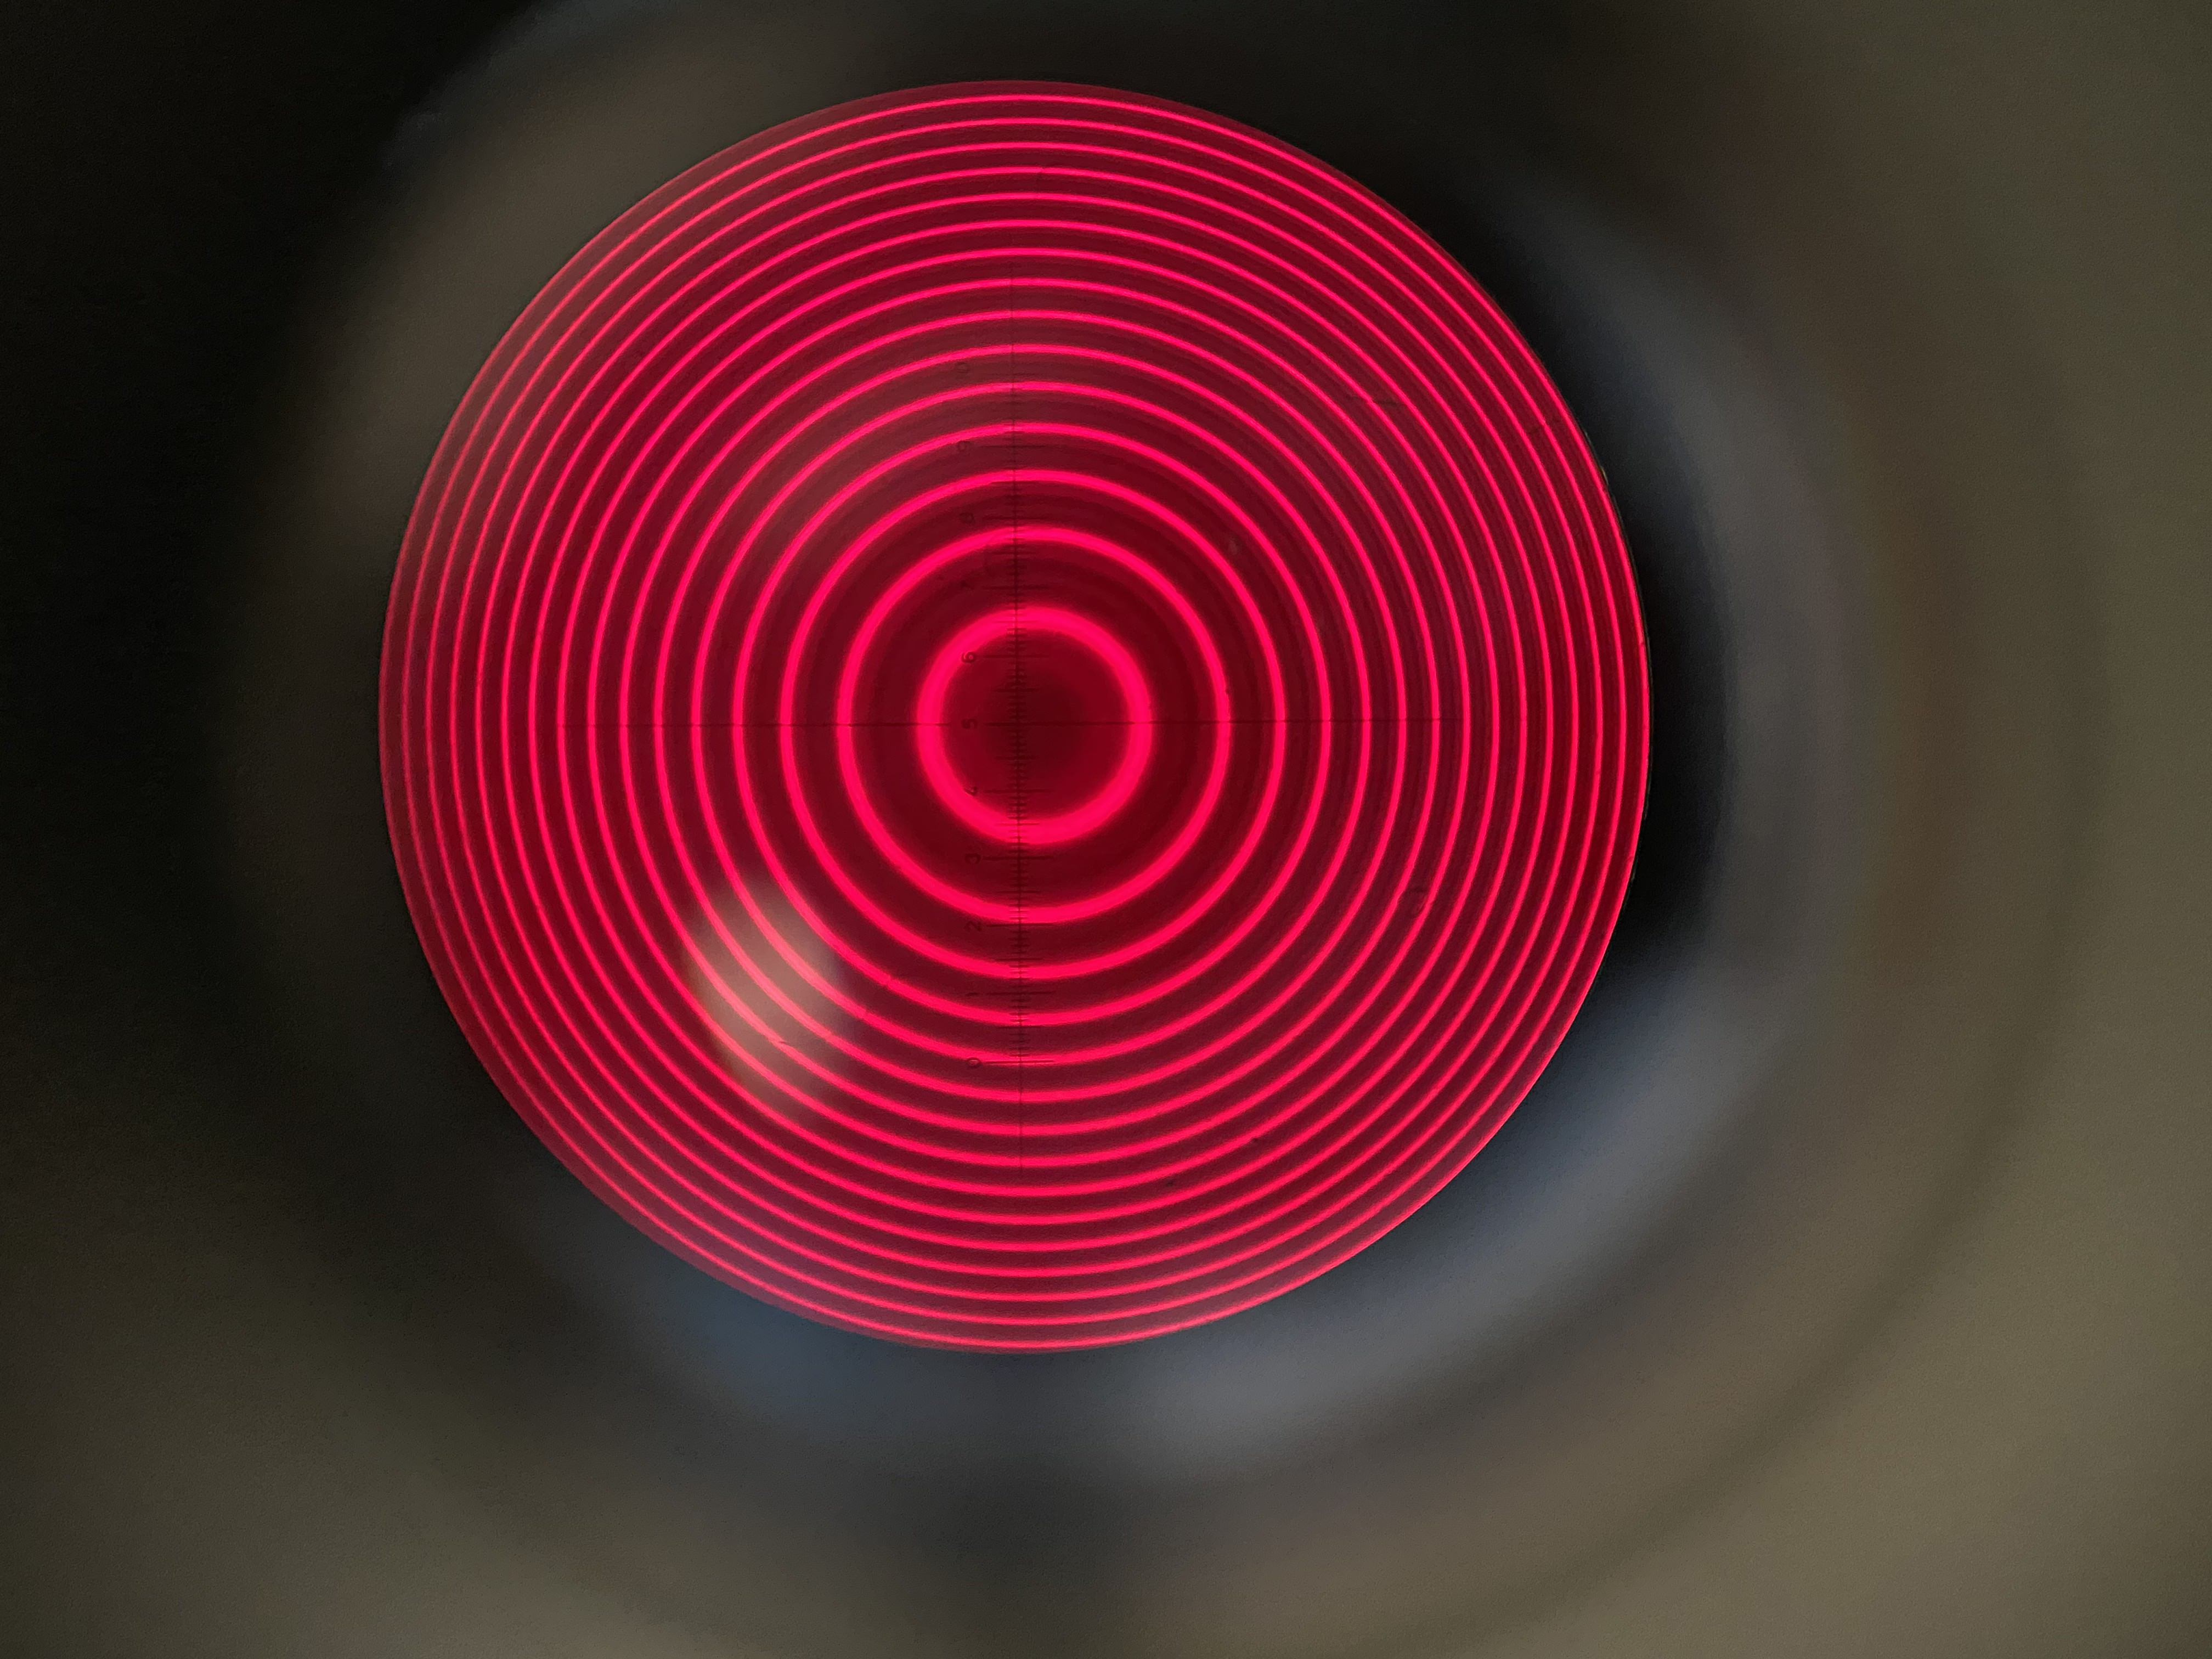
\includegraphics[width=.8\linewidth]{zeeman-longitudinal-mit--45}
  \caption{Interferenzmuster bei longitudinaler Beobachtung mit Magnetfeld, mit Polarisationsfilter.}
  \label{fig:zeeman-longitudinal-mit--45}
\end{figure}

Mit dem Polarisationsfilter in \ang{45}-Stellung ist nur der jeweils andere Ring stark zu sehen (Abb. \ref{fig:zeeman-longitudinal-mit-45}).
\begin{figure}[H]
  \centering
  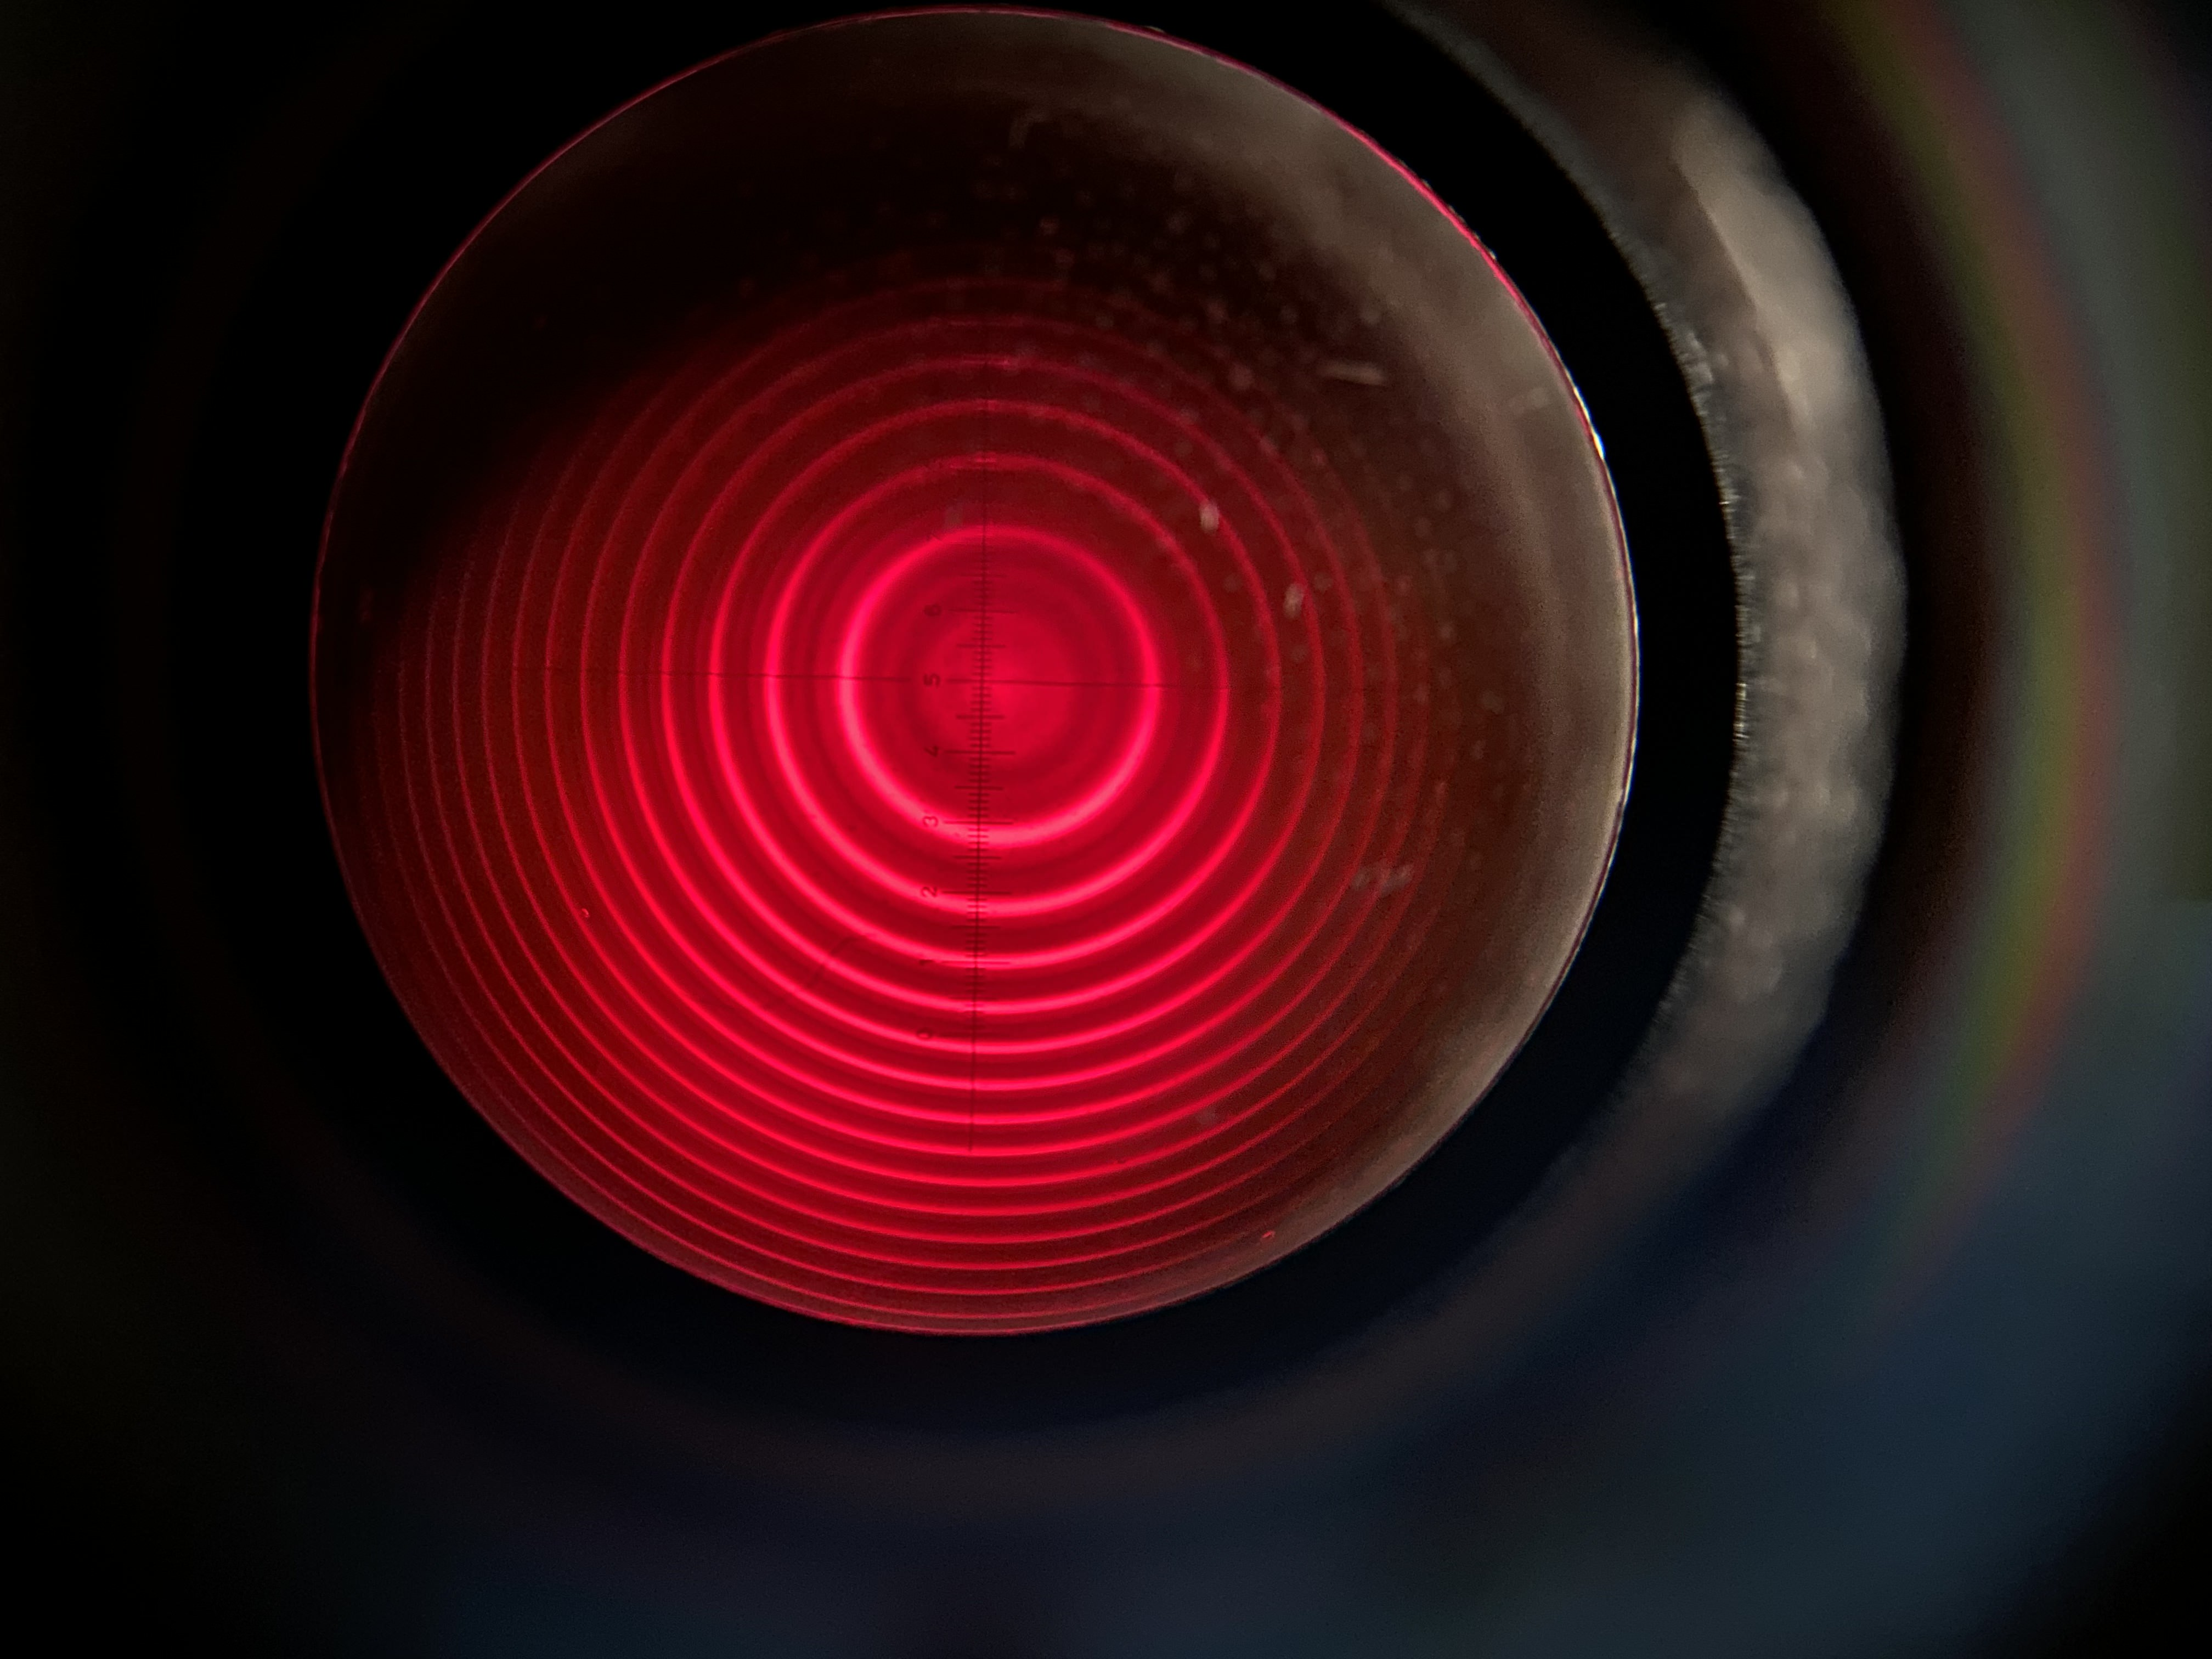
\includegraphics[width=.8\linewidth]{zeeman-longitudinal-mit-45}
  \caption{Interferenzmuster bei longitudinaler Beobachtung mit Magnetfeld, mit Polarisationsfilter.}
  \label{fig:zeeman-longitudinal-mit-45}
\end{figure}

Dies lässt sich wie folgt erklären: Die $\lambda / 4$-Platte erzeugt aus dem
rechts- bzw. linkspolarisierte Licht der $\sigma$-Übergänge
(siehe Abb. \ref{fig:zeeman-abstrahlung}) verschiedene zueinander senkrechte lineare Polarisationsrichtungen,
von denen dann mit dem Polarisationsfilter jeweils eine ausgewählt wurde.


\subsection{Auflösungsvermögen und Finesse}

Nach dem Praktikumskript ist Dicke von Fabry-Perot-Etalon 
$d = 4 \, \text{mm}$, die Mittelwellenlänge $\lambda = 643.8 \, \text{nm}$ und 
für Reflexiongrad $R=0.85$.
Damit lässt sich das theoretische Auflösungsvermögen und die Finesse $F$ 
bestimmen, es gilt dann:
\[
F_{\text{theo}} = \frac{\pi R}{1 - R^2}= 9.63
\]
\[
  A_{\text{theo}} = \frac{F \cdot 2nd}{\lambda} = 1.742 \cdot 10^5
\]

Wie im Protokoll beschrieben wird, wird der Strom so eingestellt, sodass die Aufspaltung
Spektralinien sich unterscheiden können.
\[
I_{\text{long}} = (1.2 \pm 0.1) \, \text{A}, \quad I_{\text{trans}} = (2.4 \pm 0.2) \, \text{A}
\]
Noch dazu ist der Wert des Magnetfeldes nach der Kalibrierung das Folgende: 

\[
B_{\text{long}} = ( 83.45 \pm 6.66) \, \text{mT}, \quad B_{\text{trans}} = (173.1 \pm 13.9) \, \text{mT}
\]
Dabei wurde $B$ zufolge der später erläuterten Kalibrationskurve bestimmt.

Zuletzt mit $A=\frac{hc}{\mu_B \lambda B}$ (und mit $\cdot \frac{1}{2}$ bei longitudinale 
Konfiguration) sind die jeweiligen Auflösungsvermögen und Finesse die folgende:

\[
A_{\text{trans}} = (1.88 \pm 0.14) \cdot 10^5, \quad A_{\text{long}} = (1.19 \pm 0.13) \cdot 10^5
\]

\[
  F_{\text{trans}} = 10.61 \pm 0.14 \, \text{N}, F_{\text{long}} = 6.72 \pm 0.13 \, \text{N}
\]

Unsere Werte sind ähnlich, was es zu erwarten war, denn Unsere Werte für 
$B_i$ das doppelte sind. Jedoch sind unsere beiden Werte zu niedrig gefallen und 
könnte an der Messgenauigkeit liegen. 

\subsection{Dopplerverbreiterung}
Für die Dopplerverbreiterung einer Linie durch thermische Bewegung der Atome gilt
\[
  \delta\lambda = \frac{2\lambda}{c} \sqrt{\frac{2RT\ln(2)}{M}} \cite[S. 230]{demtröder3}
\]
mit der Gaskonstante $R=\SI{8.314}{\J\per\mol\per\K}$ und der molaren Masse von Cadmium $M=\SI{112.414}{\g\per\mol}$ \cite{chemistry}
Für den $\pi$-Übergang mit $\lambda_pi^0 = \SI{643.8}{\nm}$ und der Annahme einer Temperatur von \SI{1000}{\K} ergibt sich
\[
  \delta\lambda = \SI{4.349e-5}{\nm}
\]
Die Dopplerverbreiterung ist im Verlgeich zur Wellenlänge also sehr klein.


\subsection{Messung des Zeeman-Effekts}
Es soll nun quantitativ die Stärke der Aufspaltung in Abhängigkeit des anliegenden Magnetfelds gemessen werden,
mit dem Ziel, das Bohrsche Magneton $\mu_B$ zu bestimmten.
Hierzu wird die transversale Konfiguration verwendet und $\lambda/4$-Platte sowie Polarisationsfilter aus dem Strahlengang entfernt.

\subsubsection{Magnetfeldkalibrierung}
Es wird die Abhängigkeit der Magnetfeldstärke vom fließenden Strom durchmessen, um daraus eine Kalibrierungskurve zu erstellen.
Hierzu wird anstatt der Cadmiumlampe eine Hall-Sonde genau mittig zwischen den Polschuhen eingeführt.
In Reihe zu den Magneten wird ein \enquote{Cassy-Modul} eingeschaltet,
wodurch am Computer mithilfe einer speziellen Software die Abhängigkeit automatisch aufgezeichnet werden kann.
Die Messung wird gestartet und der Strom allmählich bis zum maximal erreichbaren Wert hochgefahren.
Dann wird die Messung gestoppt und der Strom wieder ausgeschaltet.

Eine solche Kalibrierung wurde zweimal durchgeführt, einmal vor und einmal nach den Messungen aus \ref{messungmessung}.
In Abb. \ref{fig:magnetkalib} sind die Messdaten zusammen mit einem $\chi^2$-Fit der Form
\[
  B(I) = a + bI + cI^2 + dI^3
\]
dargestellt. Als Fehlerwerte auf $I$ und $B$ wurden dabei $2\%$ des jeweiligen Werts angesetzt,
wobei Fehlerwerte von $\SI{0.002}{\A}$ und $\SI{0.2}{\mT}$ nicht unterschritten werden dürfen.
Es ist anzumerken, dass die hier Strommessung mit dem hier verwendeten Cassy-Modul deutlich präzisere Werte liefert,
als das Netzgerät, welche nur eine Nachkommastelle des Stroms anzeigt.

\begin{figure}[H]
  \centering
  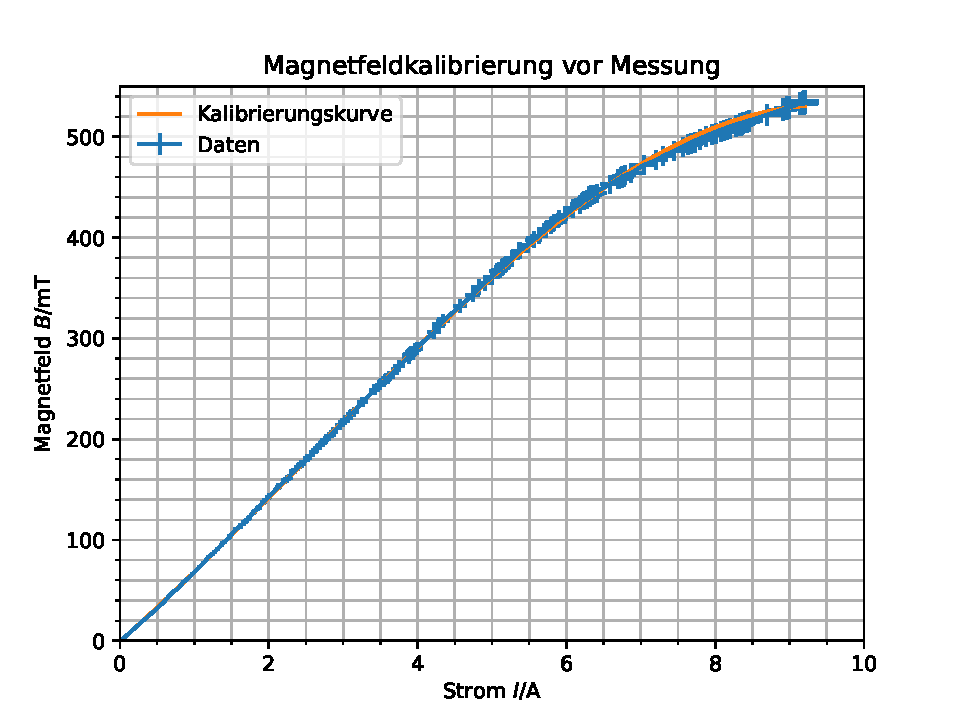
\includegraphics[width=.8\linewidth]{magnetkalib}
  \caption{Magnetfeldkalibierung vor der Messung mit CCD-Kamera}
  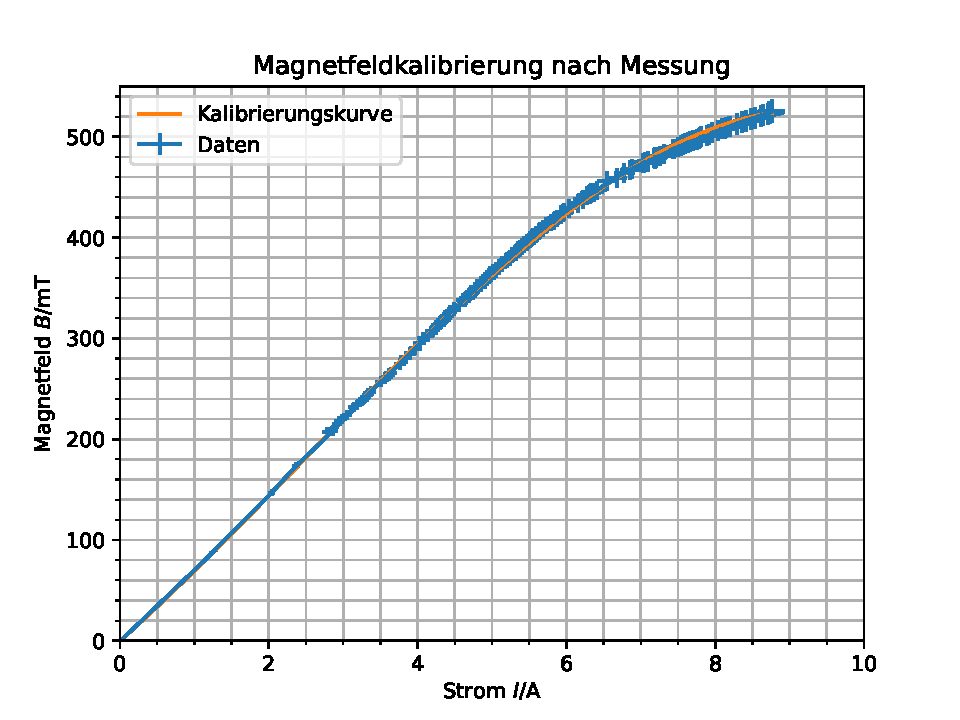
\includegraphics[width=.8\linewidth]{magnetkalib2}
  \caption{Magnetfeldkalibierung nach der Messung mit CCD-Kamera}
  \label{fig:magnetkalib}
\end{figure}

\begin{align*}
  a_1&=\SI{-0.548 \pm 0.025}{\mT},\ b_1=\SI{65.44 \pm 0.16}{\mT\per\A}, \\
  c_1&=\SI{3.964 \pm 0.065}{\mT\per\A\squared},\ d_1=\SI{-0.5213 \pm 0.0059}{\mT\per\A\cubed} \\
  a_2&=\SI{-0.104 \pm 0.027}{\mT},\ b_2=\SI{66.20 \pm 0.53}{\mT\per\A}, \\
  c_2&=\SI{3.97 \pm 0.19}{\mT\per\A\squared},\ d_2=\SI{-0.536 \pm 0.015}{\mT\per\A\cubed}
\end{align*}

Diese Werte sind in relativ guter Übereinstimmung miteinander; alle Parameter haben Überschneidungen in ihren Fehlerbereichen.
Leichte Abweichungen, z.B. beim Parameter $a$ lassen sich unter anderem dadurch erklären, dass die zweite Messung durchgeführt wurde,
als die Magnetspulen noch heiß vom vorigen Betrieb waren. Dies kann die Ergebnisse verändern.

Um eine einzelne Kalibrationskurve zu haben, verwenden wir im Folgenden die Mittelwerte der Parameter:
\begin{align*}
  % i = \frac{i_1+i_2}{2},\enspace \Delta I = \frac{\sqrt{i_1^2 + i_2^2}}{2}
  i &= \frac{i_1+i_2}{2},\enspace i=a,\,b,\,c,\,d \\
  a&=\SI{-0.326 \pm 0.019}{\mT},\ b=\SI{65.82 \pm 0.28}{\mT\per\A}, \\
  c&=\SI{3.967 \pm 0.099}{\mT\per\A\squared},\ d=\SI{-0.5288 \pm 0.0082}{\mT\per\A\cubed}
\end{align*}
Der Fehler wird dabei mithilfe von Gauß'scher Fehlerfortpflanzung bestimmt.


\subsubsection{Messungen mit CCD-Kamera} \label{messungmessung}
Die Messung der Positionen der Interferenzmaxima erfolgt mithilfe einer CCD-Kamera, die anstatt des Okulars
in den Strahlengang eingesetzt wird. Die Kamera (Auflösung von $1024$ Pixeln) wird mit dem Computer verbunden, wo mithilfe eines dafür ausgelegten
Programms die Lichtintensität in Abhängigkeit des Ablenkwinkels $\alpha$ aufgenommen wird.
Dabei wird $\alpha$ automatisch aus der Pixel-Position $p$ berechnet nach der Formel
\[
  \alpha = \arctan(\frac{(1024-p) \cdot \SI{0.014}{\mm}}{f}),\ f=\SI{150}{\mm}\ (\cite{Anleitung}, S.7)
\]

Nun wird das Magnetfeld durch Änderung des Stroms variiert und am Computer beobachtet,
wie sich die Aufspaltung der Linien verändert.
Für $10$ verschiedene Ströme wird die Messung (Werte der Intensität $I$ in Abhängigkeit des Winkels $\alpha$) jeweils abgespeichert.
Aus jeder Messung wird eine Beugungsordnung ausgesucht, bei der wir die Positionen drei verschiedenen Peaks bestimmen.
Dazu wird immer nur der Bereich dieser drei Peaks aus den Daten ausgewählt und ein Fit der Form
% Dies erfolgt mithilfe eines Dreifachen Gauß-Fits der Form
\[
  I(\alpha) = B + G(\alpha; a_1, \mu_1, \sigma_1) + G(\alpha; a_2, \mu_2, \sigma_2) + G(\alpha; a_3, \mu_3, \sigma_3)
\]
durchgeführt. Dabei wurde auf den Intensitäten ein Fehler von $\Delta I = 1\%$ angenommen.
Der additive Parameter $B$ ermöglicht die Berücksichtigung einer eventuell vorhanden gleichmäßigen Grundausleuchtung
und sorgt nach visueller Inspektion erfahrungsgemäß für bessere Anpassung der Gauß-Parameter an die Daten.
Es werden die verallgemeinerten Gauß-Funktionen
\[
  G(xg a, \mu, \sigma) = a \exp(\frac{(x-b)^2}{2c^2})
\]
verwendet. 
Die Plots mit Fit sind in Abb. \ref{fig:gauss-fit-1} und \ref{fig:gauss-fit-2} gezeigt, die Parameter in Tab. \ref{tab:parameter}.

Für die Energiedifferenz gilt
\[
  \Delta E_\pm = -\frac{h c}{\lambda_\pi} \frac{\lambda_\sigma - \lambda_\pi}{\lambda_\sigma} \cite{Anleitung}
\]
mit $\lambda_pi^0 = \SI{643.8}{\nm}$ \cite{Leybold}.
Einsetzen der Interferenzbedingung \eqref{eq:fpi-interferenz}
\[
  \Delta E_\pm = -\frac{h c}{\lambda_\pi} (1 - \frac{\sqrt{n^2-\sin^2(\alpha_\pi)}}{\sqrt{n^2-\sin^2(\alpha_\sigma)}})
\]

Die Werte, die sich hieraus ergeben, sind, zusammen mit den aus der Kalibrationskurve bestimmten B-Werten, sind in Tab. \ref{tab:zeeman-energies} gezeigt.
Dabei ist $\Delta E$ jeweils der Mittelwert aus $\Delta E_-$ und $\Delta E_+$. Die Fehler wurden mit Gauß'scher Fehlerfortpflanzung berechnet.
% Die Werte, die sich hieraus ergeben, sind, zusammen mit den aus der Kalibrationskurve bestimmten B-Werten, sind in der untenstehenden Abbildung geplottet.

% Dabei ist $\Delta E$ jeweils der Mittelwert aus $\Delta E_-$ und $\Delta E_+$.

% \begin{table}
%   \centering
%   \csvreader[
%     table head=\hline $B$ & $\Delta B$ & $\Delta E_-$ & $\Delta (\Delta E_-)$ & $\Delta E_+$ & $\Delta (\Delta E_+)$ & $\Delta E$ & $\Delta (\Delta E)$\\,
%     tabular=|c||c|c||c|c||c|c||,
%     late after line=\\\hline,
%     head to column names
%   ]{../data/energy_data.csv}{}%
%   {\csvcoli & \csvcolii & \csvcoliii}
  
\begin{table}[H]
    \centering
    \begin{tabular}{cccc}
        \toprule
        $B/\si{\mT}$ & $\Delta B/\si{\mT}$ & $\Delta E/\si{\J}$ & $\Delta \Delta E/\si{\J}$ \\
        \midrule
        \num{124.9236} & \num{11.885} & \num{9.338e-5} & \num{4.655e-7} \\
        \num{191.4964} & \num{12.705} & \num{9.391e-5} & \num{8.974e-7} \\
        \num{256.4708} & \num{14.110} & \num{8.479e-5} & \num{3.411e-7} \\
        \num{316.6740} & \num{16.246} & \num{8.945e-5} & \num{1.225e-7} \\
        \num{368.9332} & \num{19.199} & \num{9.376e-5} & \num{1.565e-7} \\
        \num{410.0756} & \num{23.002} & \num{9.592e-5} & \num{1.685e-7} \\
        \num{425.4865} & \num{25.223} & \num{9.666e-5} & \num{1.710e-7} \\
        \num{436.9284} & \num{27.656} & \num{9.721e-5} & \num{1.734e-7} \\
        \num{444.0047} & \num{30.300} & \num{9.779e-5} & \num{1.714e-7} \\
        \num{446.1753} & \num{33.751} & \num{9.883e-5} & \num{1.912e-7} \\
        \bottomrule
    \end{tabular}
    \caption{Magnetfeldstärken und zugehörige Energieverschiebungen.}
    \label{tab:zeeman-energies}
\end{table}

Wir tragen $\Delta E$ gegen $B$ auf und passen eine Gerade daran an. Nach \eqref{eq:delta-e} (mit $\Delta m_J=1$)
entspricht die Steigung dieser Geraden dem Bohrschen Magneton $\mu_B$.



\begin{figure}[H]
  \centering
  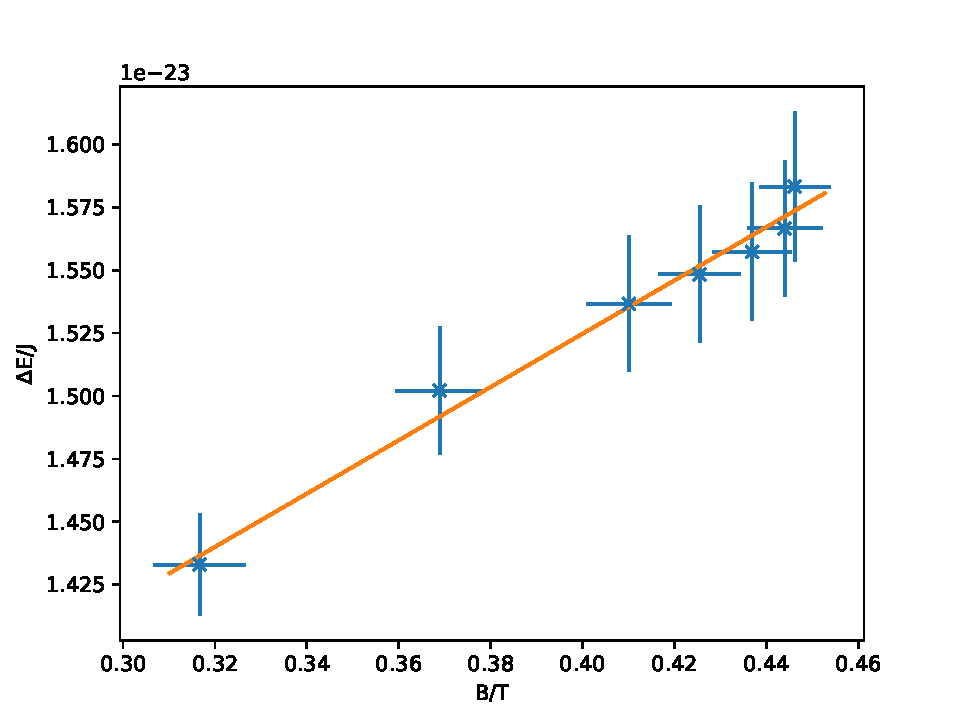
\includegraphics[width=\linewidth]{energy_plot.pdf}
\end{figure}
aus einem linearen $\chi^2$-Fit erhalten wir die Gleichung
\[
  \Delta E = \SI{1.100\pm 0.050 e-23}{\J} + \SI{1.06\pm 0.13 e-23}{\J\per\T}
\]
also ist das Ergebnis $\mu_B = \SI{1.06\pm 0.15e-23}{\J\per\T}$.

Der Literaturwert für das Bohrsche Magneton ist $\SI{0.927e-23}{\J\per\T}$ \cite{bohr-magneton}, was im Fehlerbereich unseres Wertes liegt,
aber eine relativ große Abweichung von über $10\%$ hat.
Abweichungen bei dieser Messung lassen sich unter anderem darauf zurückführen, dass der Strom am Netzgerät abgelesen wurde,
während er zur Magnetfeldkalibierung mit einem zusätzlichen Gerät gemessen wurde. Zwischen diesen beiden Messungen kann
es Abweichungen geben, und Die Messung des Netzgeräts ist relativ unpräzise (ablesbar ist nur eine Nachkommastelle).

Es fällt außerdem der große Achsenabschnitt der Gerade auf, der dem theoretischen Zusammenhang zufolge eigentlich $0$
sein sollte. Dieser ließe sich unter anderem durch einen konstanten Offset in der, wie zuvor erwähnt ungenauen, Stromangabe des
Netzgeräts, erklären. Dieser würde einen konstanten Offset des Magnetfelds hinzufügen,
würde aber die Abstände zwischen Magnetfeldwerten und damit die errechnete Steigung $\mu_B$
nicht stark beeinflussen, da die Kalibrationskurve in großen Bereichen linear ist.


\clearpage
\section{Franck-Hertz-Versuch}
Im folgenden Abschnitt wird das Franck-Hertz-Experiment durchgeführt und anschließend detailliert 
diskutiert. Anhand der durch das Cassy-Modul gemessenen Anodenstromkurven \( I_A \) wird die 
Energiedifferenz \( \Delta E \) zwischen den Energieniveaus des Quecksilbers $Hg$, \( 6S \) und \( 6P \), 
präzise bestimmt.
\subsection{Aufbau}
In einer Franck-Hertz-Röhre, die mit Quecksilbers gefüllt ist, befindet sich eine glühende 
Kathode mit einer Heisspannung $U_H$, die die Elektronen durch thermische Emmission freisetzt und in der 
Richtung einer positiv geladenen Anode beschleunigt. Die Beschleunigungsspannung $U_B$ zwischen Kathode 
und Anode bestimmt die kinetische Energie der Elektronen, bevor sie auf die Quecksilberatome treffen.

Zwischen der Kathode und der Anode befindet sich ein Gitter, das in einigen Konstruktionen mit einem kleinen 
Gegenfeld ausgestattet ist. Dieses ist dafür verantwortlich, ob ein Elektron bis zum Auffängergitter 
gestoppt wird oder gelangen wird. Somit dürfen nur Elektronen, die genaue Energie besitzen
durch die Gitteranode. 
\\Der Anodenstrom $I_A$
wird dann in Abhängigkeit von der Spannung $U_B$ gemessen. Bei bestimmten Spannungswerten zeigt 
der Anodenstrom charakteristische Einbrüche, die auftreten, wenn die Elektronen genau die Energie 
erreichen, die nötig ist, um ein Quecksilberatom vom Grundzustand (6S) in einen angeregten 
Zustand (6P) zu heben.
 Durch diesen inelastischen Stoß verlieren die Elektronen ihre kinetische Energie und tragen dadurch nicht mehr zum Stromfluss bei.

Die Spannungsdifferenz zwischen aufeinanderfolgenden Strommaxima liefert die Energie $\Delta E$, die den 
Übergang zwischen den 6S- und 6P-Niveaus beschreibt. 
\subsection{Durchführung und Auswertung}
Zunächst wird die Energiedifferenz $\Delta E$ zwischen die Energieniveaus des $Hg$ bestimmt. 
Dabei sollen die Breiten der Kurven bzw. die Peaks bestimmt werden. Dazu werden Gaußkurven an die Daten angepasst,
die mithilfe des Programms \textit{Fityk} gemacht werden.
\\ Es ist zu beachten, dass bei den verschiedenen Messungen nicht dieselbe Anzahl an Peaks 
erfasst wurde. Daher wurden nur die erkennbaren Peaks analysiert und in die Tabellen 
aufgenommen. 
\subsection*{Fityk Version 1.3.1}
In \textit{Fityk} werden Gauß-Fits durch Auswahl eines Datenbereichs und Anwendung einer Gaußfunktion als 
Modell durchgeführt. Die Gaußfunktion hat die Form 

\begin{equation*}
f(x) = a \cdot e^{-\frac{(x - \mu)^2}{2 \sigma^2}}
\end{equation*}
wobei $a$ die Amplitude, $\mu$ der Mittelwert (Zentrum des Peaks) und $\sigma$ die Standardabweichung 
ist. Das Programm optimiert die Parameter $a$, $\mu$ und $\sigma$, sodass die Abweichung zwischen dem Modell 
und den Datenpunkten minimiert wird. Die Methode der kleinsten Quadrate wird oft verwendet, um den
 Fehlerausdruck
\begin{equation*}
\sum_{i=1}^{N} (y_i - f(x_i))^2
\end{equation*}
zu minimieren, wobei $y_i$ die gemessenen Datenpunkte und $f(x_i)$ die entsprechenden Werte der Gaußfunktion 
sind. Dadurch entsteht eine Gaußkurve, die die Daten im ausgewählten Bereich bestmöglich beschreibt.
\subsection*{Diskussion der Daten}
 Wie bereits erwähnt, wurde während des Experiments nicht dieselbe Anzahl von Peaks erfasst. Dies stellt jedoch 
 kein Problem dar, da eine ausreichende Anzahl an Messwerten vorliegt. Zudem wurde in \textit{Fityk} eine 
 Hintergrundfunktion zu den Gauß-Fits hinzugefügt, sodass die Gesamtsumme der Gauß-Peaks eine bessere 
 Übereinstimmung mit den im Experiment beobachteten Peaks aufweist. Unter Berücksichtigung der oben genannten Anpassungen 
 und Messmethoden folgen nun die entsprechenden Graphen. Die Fits aus Fityk lassen sich im Anhang anschauen. 
\begin{figure}[H]
  \centering
  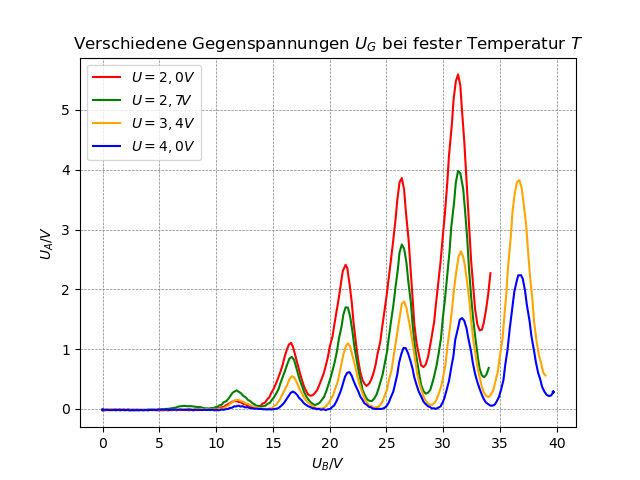
\includegraphics[scale=0.55]{FH_vieleT.png}
  \caption{Die gemessene  Anodenspannung $U_A$ gegen Beschleunigungsspannung $U_B$ bei
   verschiedene Gegenspannung $T$ und fester Temperatur $U_G$}
\end{figure}

\begin{figure}[H]
  \centering
  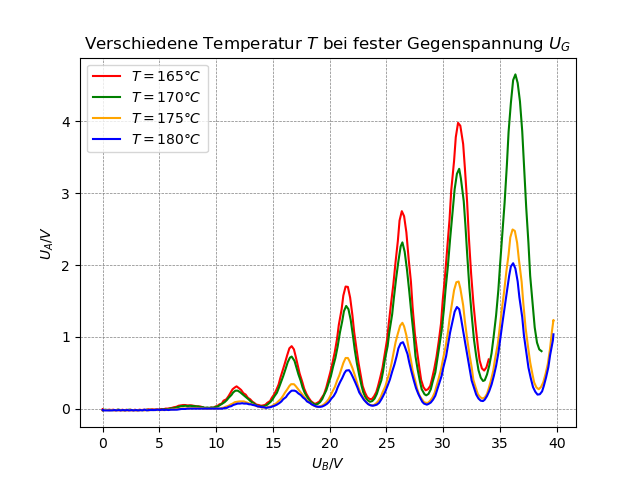
\includegraphics[scale=0.55]{FH_vieleU.png}
  \caption{Die gemessene Anodenspannung $U_A$ gegen Beschleunigungsspannung $U_B$
  verschiedenen Temperaturen $T$ und Gegenspannung $U_G$}
\end{figure}

\subsection*{Bestimmung der Energiedifferenz}
Zunächst wird aus den Werten der Spannungen $U_B^i$ ausgerechnet. Um die Eindeutigkeit von diesen 
zu gewährleisten, bezeichnen wir die Peaks bzw. die Erwartungswerte mit $U^i_B$ und 
fassen alle relevanten Informationen in einer Tabelle zusammen.
Der Fehler des Mittelwerts wird durch die folgende Formel und in der Tabelle dargestellt:
\begin{equation*}
\Delta(U^i_B) = \sqrt{\frac{1}{N} \sum_{n=1}^{N} \left( \delta U_{i,n}^B \right)^2}
\end{equation*}
Dabei ist \( N \) die Anzahl der Werte, die zur Berechnung des Mittelwerts beitragen.

Im Folgenden sind die Mittelwerte der Beschleunigungsspannung sowie die entsprechenden Fehler dargestellt.
\begin{table}[H]
  \centering
  \begin{tabular}{cc} 
      \hline
      & Mittelwert [V] \\ \hline
      $U^1_B$ & 36.3 \\ \hline
      $U^2_B$ & 31.2 \\ \hline
      $U^3_B$ & 26.3 \\ \hline
      $U^4_B$ & 21.6 \\ \hline
      $U^5_B$ & 16.6 \\ \hline
      $U^6_B$ & 11.8 \\ \hline
  \end{tabular}
  \caption{Mittelwerte zu $U^i_B$}
  \label{tab:median_values}
\end{table}

\begin{table}[H]
  \centering
  \begin{tabular}{cc} 
      \hline
       & Mittelwert [V] \\ \hline
      $\delta U^1_B$ & $\pm 0.0504$ \\ \hline
      $\delta U^2_B$ & $\pm 0.133$ \\ \hline
      $\delta U^3_B$ & $\pm 0.0112$ \\ \hline
      $\delta U^4_B$ & $\pm 0.0161$ \\ \hline
      $\delta U^5_B$ & $\pm 0.0307$ \\ \hline
      $\delta U^6_B$ & $\pm 0.131$ \\ \hline
  \end{tabular}
  \caption{Mittelwerte zu $\delta U^i_B$}
  \label{tab:mean_values}
\end{table}
Nun kann man aus den Diferenzen der benachbaren Peaks der Energiedifferenz $\Delta E$ bestimmt werden. 
\begin{equation*}
  \Delta E=(4.9 \pm 0.0803)eV
\end{equation*}
Das Ergebnis unserer experimentellen Messungen ist äußerst erfreulich und stimmt vollständig 
mit dem erwarteten theoretischen Wert der Übergang zwischen $6^1 S_o \rightarrow 6^3P_1$ überein. 
Wie man in der Abbildung sich anschauen kann. Es wäre möglicherweise sinnvoller gewesen, zunächst 
die Energiedifferenzen zu berechnen und anschließend einen Mittelwert zu bilden, da die Positionen 
der Peaks in der Funktion nicht konstant sind. Da jedoch die Anzahl der Peaks in den verschiedenen 
Messungen nicht übereinstimmt, erscheint die gewählte Vorgehensweise in diesem Fall besser geeignet.\\

Untersucht man den Zusammenhang zwischen der Energiedifferenz und dem Wirkungsquerschnitt 
(siehe Abbildung \ref{Wirkungsquerschnitt}), so zeigt sich, dass die Übergangsenergien von 
1 bis 3 kaum voneinander zu unterscheiden sind. Es wird jedoch deutlich, dass der zweite Übergang wesentlich wahrscheinlicher ist 
als die anderen, da sein Wirkungsquerschnitt deutlich größer ist als der des ersten Übergangs.

Andere Übergänge können ebenfalls stattfinden, treten jedoch seltener auf. Insbesondere der vierte Übergang ist möglich, 
kommt jedoch aufgrund des höheren Energiebedarfs deutlich seltener vor.
\begin{figure}[H]
  \centering
  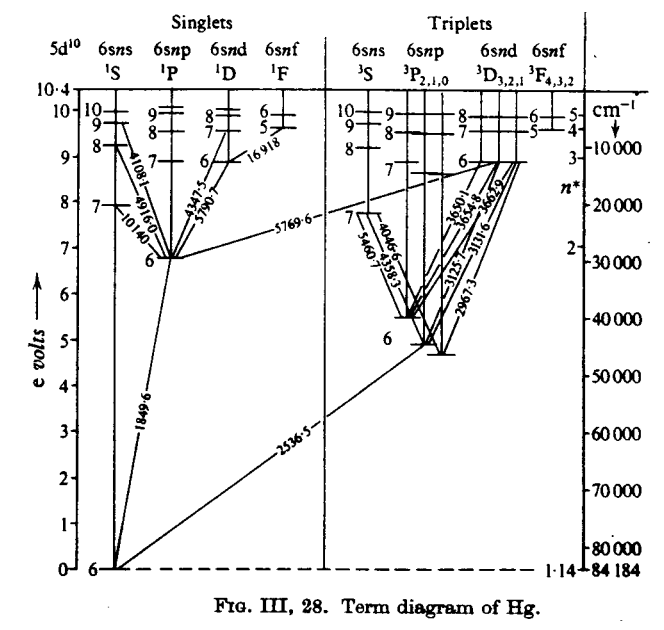
\includegraphics[scale=0.45]{Vereinfachtes Hg-Termschema.png}
  \caption{Termschema des Quecksilbers}
\end{figure}
\subsection{Einfluss der Temperatur $T$}
Zudem erkennt man mithilfe des Anhangs im Praktikumskript, dass der Dampfdruck von 
Quecksilber stark von der Temperatur abhängt (siehe untenstehende Formel).

\begin{equation*}
  log(p) = 10.55 - \frac{3333}{T} - 0.85log(T)
\end{equation*}
Daraus folgt, dass bei steigender Temperatur vermehrt thermische Stöße zwischen den H
g-Atomen stattfinden können, was dazu führt, dass weniger Elektronen die notwendige 
Energie besitzen, um die Anode zu erreichen. Andererseits treten bei niedrigeren 
Temperaturen zu weniger inelastische Stöße auf, was zur Folge hat, dass man keine sinnvolle
Messung bekommt.

\begin{figure}[H]
  \centering
  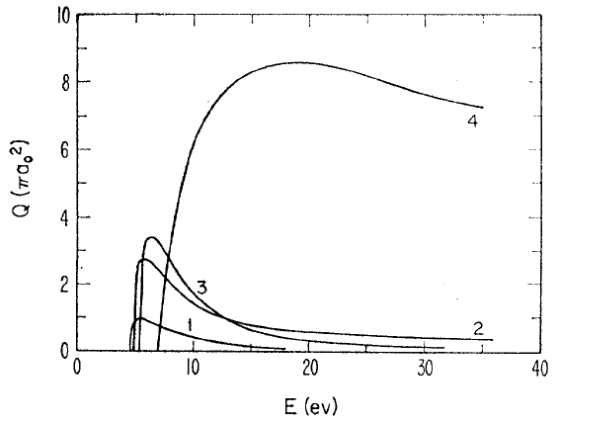
\includegraphics[scale=0.55]{Totaler Wirkungsquerschnitt.png}
  \caption{Totaler Wirkungsquerschnitt $Q(\pi a^2_0$) von Hg für Elektronenstoßanregung}
  \label{Wirkungsquerschnitt}
\end{figure}
\clearpage
\section{Fazit}
Anhand der Energiedifferenz zwischen $\pi$- und $\sigma$-Übergängen zwischen dem $^1D_2$ und dem $^1P_1$-Zustand
von Cadmium konnte das Bohrsche Magneton auf $\mu_B = \SI{1.06\pm 0.15e-23}{\J\per\T}$ bestimmt werden,
wobei der Literaturwert von $\SI{0.927e-23}{\J\per\T}$ \cite{bohr-magneton} im Fehlerbereich liegt.
Die relativ große Abweichung von über $10\%$ lässt sich unter anderem durch die ungenaue Strommessung
des Netzgerätes erklären.
Zur Interferometrie wurde ein Fabry-Perot-Etalon verwendet, anhand dessen Interferenzbild die Positionen der Intensitätsmaxima
bei verschieden starken Magnetfeldern verglichen wurden. Die Messung wurde mithilfe einer CCD-Kamera durchgeführt.

Im zweiten Versuchsteil wird der Franck-Hertz-Versuch aufgebaut und untersucht. Dabei 
wird die Beschleunigungsspannung in Abhängigkeit von der Anodenspannung bei verschiedenen 
Temperaturen und Gegenspannungen aufgezeichnet, wodurch die erwarteten Peaks entstehen. 
Mithilfe der Berechnung des Erwartungswerts $\mu_i$ und der Standardabweichung $\sigma_i$ 
wird nach der Datenanalyse festgestellt, dass die Energiedifferenz für den Übergang im 
Hg-Atom zwischen den Zuständen $6^1S_0$ und $6^3P_1$ den Wert $\Delta E = (4.9 \pm 0.0803) \, 
\text{eV}$ annimmt, was erstaunlich gut mit dem theoretischen Wert übereinstimmt. Zudem 
fällt auf, dass bei erhöhter Temperatur $T$ und Gegenspannung $U_G$ die Anodenspannung $U_A$ abnimmt.





\clearpage
\section{Anhang}
\begin{table}[H]
  \centering
  \begin{tabular}{|c|c|c|}
      \hline
      Parameter & Wert & Fehler $\Delta$ \\ \hline
      $\mu_1$ & 31.1 & $\pm$ 0.0183 \\ \hline
      $\sigma_1$& 1.26 & $\pm$ 0.0358 \\ \hline
      $\mu_2$ & 26.1 & $\pm$ 0.0162 \\ \hline
      $\sigma_2$ & 1.08 & $\pm$ 0.0249 \\ \hline
      $\mu_3$ & 21.2 & $\pm$ 0.024 \\ \hline
      $\sigma_3$ & 0.91 & $\pm$ 0.0298 \\ \hline
      $\mu_4$ & 16.4 & $\pm$ 0.0365 \\ \hline
      $\sigma_4$ & 0.843 & $\pm$ 0.0522 \\ \hline
      $\mu_5$ & 11.7 & $\pm$ 0.237 \\ \hline
      $\sigma_5$ & 0.669 & $\pm$ 0.306 \\ \hline
  \end{tabular}
  \caption{Parameter bei $U_G=2.0V$ und $T=165^\circ C$}
  \label{tab:data_no_height}
\end{table}
\begin{table}[H]
  \centering
  \begin{tabular}{|c|c|c|}
      \hline
      Parameter & Wert & Fehler $\Delta$ \\ \hline
      $\mu_1$ & 31.3 & $\pm$ 0.00925 \\ \hline
      $\sigma_1$ & 1.04 & $\pm$ 0.0129 \\ \hline
      $\mu_2$ & 26.3 & $\pm$ 0.00979 \\ \hline
      $\sigma_2$ & 0.967 & $\pm$ 0.0151 \\ \hline
      $\mu_3$ & 21.4 & $\pm$ 0.0133 \\ \hline
      $\sigma_3$ & 0.914 & $\pm$ 0.019 \\ \hline
      $\mu_4$ & 16.6 & $\pm$ 0.0242 \\ \hline
      $\sigma_4$ & 0.885 & $\pm$ 0.0321 \\ \hline
      $\mu_5$ & 11.9 & $\pm$ 0.0715 \\ \hline
      $\sigma_5$ & 0.884 & $\pm$ 0.0916 \\ \hline
  \end{tabular}
  \caption{Parameter bei $U_G=2.7V$ und $T=165^\circ C$}
  \label{tab:data_no_height_2}
\end{table}

\begin{table}[H]
  \centering
  \begin{tabular}{|c|c|c|}
      \hline
      Parameter & Wert & Fehler $\Delta$ \\ \hline
      $\mu_1$ & 36.7 & $\pm$ 0.00818 \\ \hline
      $\sigma_1$ & 1.19 & $\pm$ 0.00971 \\ \hline
      $\mu_2$ & 31.6 & $\pm$ 0.0125 \\ \hline
      $\sigma_2$ & 1.02 & $\pm$ 0.0153 \\ \hline
      $\mu_3$ & 26.5 & $\pm$ 0.0121 \\ \hline
      $\sigma_3$ & 0.95 & $\pm$ 0.0143 \\ \hline
      $\mu_4$ & 21.6 & $\pm$ 0.0181 \\ \hline
      $\sigma_4$ & 0.871 & $\pm$ 0.0215 \\ \hline
      $\mu_5$ & 16.7 & $\pm$ 0.0362 \\ \hline
      $\sigma_5$ & 0.846 & $\pm$ 0.0423 \\ \hline
  \end{tabular}
  \caption{Parameter bei $U_G=3.4V$ und $T=165^\circ C$}
  \label{tab:data_no_height_3}
\end{table}

\begin{table}[H]
  \centering
  \begin{tabular}{|c|c|c|}
      \hline
      Parameter & Wert & Fehler $\Delta$ \\ \hline
      $\mu_1$ & 36.8 & $\pm$ 0.00835 \\ \hline
      $\sigma_1$ & 1.0 & $\pm$ 0.0123 \\ \hline
      $\mu_2$ & 31.7 & $\pm$ 0.00744 \\ \hline
      $\sigma_2$ & 0.944 & $\pm$ 0.00934 \\ \hline
      $\mu_3$ & 26.7 & $\pm$ 0.00927 \\ \hline
      $\sigma_3$ & 0.837 & $\pm$ 0.0111 \\ \hline
      $\mu_4$ & 21.7 & $\pm$ 0.0151 \\ \hline
      $\sigma_4$ & 0.769 & $\pm$ 0.0178 \\ \hline
      $\mu_5$ & 16.8 & $\pm$ 0.0313 \\ \hline
      $\sigma_5$ & 0.712 & $\pm$ 0.0371 \\ \hline
  \end{tabular}
  \caption{Parameter bei $U_G=4.0V$ und $T=165^\circ C$}
  \label{tab:data_no_height_5}
\end{table}

\begin{table}[H]
  \centering
  \begin{tabular}{|c|c|c|}
      \hline
      Parameter & Wert & Fehler $\Delta$ \\ \hline
      $\mu_1$ & 36.3 & $\pm$ 0.00915 \\ \hline
      $\sigma_1$ & 1.11 & $\pm$ 0.0139 \\ \hline
      $\mu_2$ & 31.2 & $\pm$ 0.00858 \\ \hline
      $\sigma_2$ & 1.02 & $\pm$ 0.0136 \\ \hline
      $\mu_3$ & 26.3 & $\pm$ 0.0105 \\ \hline
      $\sigma_3$ & 0.966 & $\pm$ 0.0152 \\ \hline
      $\mu_4$ & 21.4 & $\pm$ 0.0148 \\ \hline
      $\sigma_4$ & 0.92 & $\pm$ 0.0205 \\ \hline
      $\mu_5$ & 16.6 & $\pm$ 0.0277 \\ \hline
      $\sigma_5$ & 0.889 & $\pm$ 0.0364 \\ \hline
      $\mu_6$ & 11.9 & $\pm$ 0.0832 \\ \hline
      $\sigma_6$ & 0.893 & $\pm$ 0.106 \\ \hline
  \end{tabular}
  \caption{Parameter bei $U_G=2.7V$ und $T=170^\circ C$}
  \label{tab:data_no_height_6}
\end{table}

\begin{table}[H]
  \centering
  \begin{tabular}{|c|c|c|}
      \hline
      Parameter & Wert & Fehler  \\ \hline
      $\mu_1$ & 36.3 & $\pm$ 0.128 \\ \hline
      $\sigma_1$ & 1.67 & $\pm$ 0.212 \\ \hline
      $\mu_2$ & 30.8 & $\pm$ 0.734 \\ \hline
      $\sigma_2$ & 1.08 & $\pm$ 0.26 \\ \hline
      $\mu_3$ & 26.3 & $\pm$ 0.0108 \\ \hline
      $\sigma_3$ & 0.929 & $\pm$ 0.0138 \\ \hline
      $\mu_4$ & 21.5 & $\pm$ 0.0112 \\ \hline
      $\sigma_4$ & 0.981 & $\pm$ 0.0135 \\ \hline
      $\mu_5$ & 16.8 & $\pm$ 0.0232 \\ \hline
      $\sigma_5$ & 1.00 & $\pm$ 0.0275 \\ \hline
  \end{tabular}
  \caption{Parameter bei $U_G=2.7V$ und $T=175^\circ C$}
  \label{tab:data_no_height_7}
\end{table}

\begin{table}[H]
  \centering
  \begin{tabular}{|c|c|c|}
      \hline
      Parameter & Wert & Fehler  \\ \hline
      $\mu_1$ & 36.1 & $\pm$ 0.00659 \\ \hline
      $\sigma_1$ & 0.952 & $\pm$ 0.0118 \\ \hline
      $\mu_2$ & 31.2 & $\pm$ 0.00694 \\ \hline
      $\sigma_2$ & 0.968 & $\pm$ 0.0108 \\ \hline
      $\mu_3$ & 26.3 & $\pm$ 0.0095 \\ \hline
      $\sigma_3$ & 0.921 & $\pm$ 0.0152 \\ \hline
      $\mu_4$ & 21.6 & $\pm$ 0.016 \\ \hline
      $\sigma_4$ & 0.893 & $\pm$ 0.0233 \\ \hline
      $\mu_5$ & 16.8 & $\pm$ 0.0351 \\ \hline
      $\sigma_5$ & 0.911 & $\pm$ 0.0544 \\ \hline
  \end{tabular}
  \caption{Parameter bei $U_G=2.7V$ und $T=180^\circ C$}
  \label{tab:data_no_height_8}
\end{table}

\begin{table}[H]
  \centering
  \begin{tabular}{cccccc} 
      \hline
      $U^1_B$[V] & $U^2_B$[V] & $U^3_B$[V] & $U^4_B$[V] & $U^5_B$[V] & $U^6_B$[V] \\ \hline
      36.7 & 31.1 & 26.1 & 21.2 & 16.4 & 11.7 \\ \hline
      36.8 & 31.3 & 26.3 & 21.4 & 16.6 & 11.9 \\ \hline
      36.3 & 31.6 & 26.5 & 21.6 & 16.7 & 11.9 \\ \hline
      36.3 & 31.7 & 26.7 & 21.7 & 16.6 & - \\ \hline
      36.1 & 31.2 & 26.3 & 21.4 & 16.8 & - \\ \hline
      - & 30.8 & 26.3 & 21.5 & 16.8 & - \\ \hline
      - & 31.2 & 26.3 & 21.6 & 16.8 & - \\ \hline
  \end{tabular}
  \caption{zugeordnete $U^i_B$}
  \label{tab:measurements}
\end{table}

\begin{table}[H]
  \centering
  \small 
  \begin{tabular}{cccccc} 
      \hline
      $\delta U^1_B$[V] & $\delta U^2_B$[V] & $\delta U^3_B$[V] & $\delta U^4_B$[V] & $\delta U^5_B$[V] & $U^6_B$[V] \\ \hline
      $\pm 0.00818$ & $\pm 0.0183$ & $\pm 0.0162$ & $\pm 0.024$ & $\pm 0.0365$ & $\pm 0.237$ \\ \hline
      $\pm 0.00835$ & $\pm 0.00925$ & $\pm 0.00979$ & $\pm 0.0133$ & $\pm 0.0242$ & $\pm 0.0715$ \\ \hline
      $\pm 0.00915$ & $\pm 0.0125$ & $\pm 0.0121$ & $\pm 0.0181$ & $\pm 0.0362$ & $\pm 0.0832$ \\ \hline
      $\pm 0.128$ & $\pm 0.00744$ & $\pm 0.00927$ & $\pm 0.0151$ & $\pm 0.0313$ & - \\ \hline
      $\pm 0.00659$ & $\pm 0.00858$ & $\pm 0.0105$ & $\pm 0.0148$ & $\pm 0.0277$ & - \\ \hline
      - & $\pm 0.734$ & $\pm 0.0108$ & $\pm 0.0112 $ & $\pm 0.0232$ & - \\ \hline
      - & $\pm 0.00694$ & $\pm 0.0095$ & $\pm 0.016$ & $\pm 0.0351$ & - \\ \hline
  \end{tabular}
  \caption{zugeordnete $\delta U^i_B$}
  \label{tab:measurements}
\end{table}

\end{multicols}



\begin{figure}[h]
  \centering
  \begin{minipage}{.49\linewidth}
    \centering
    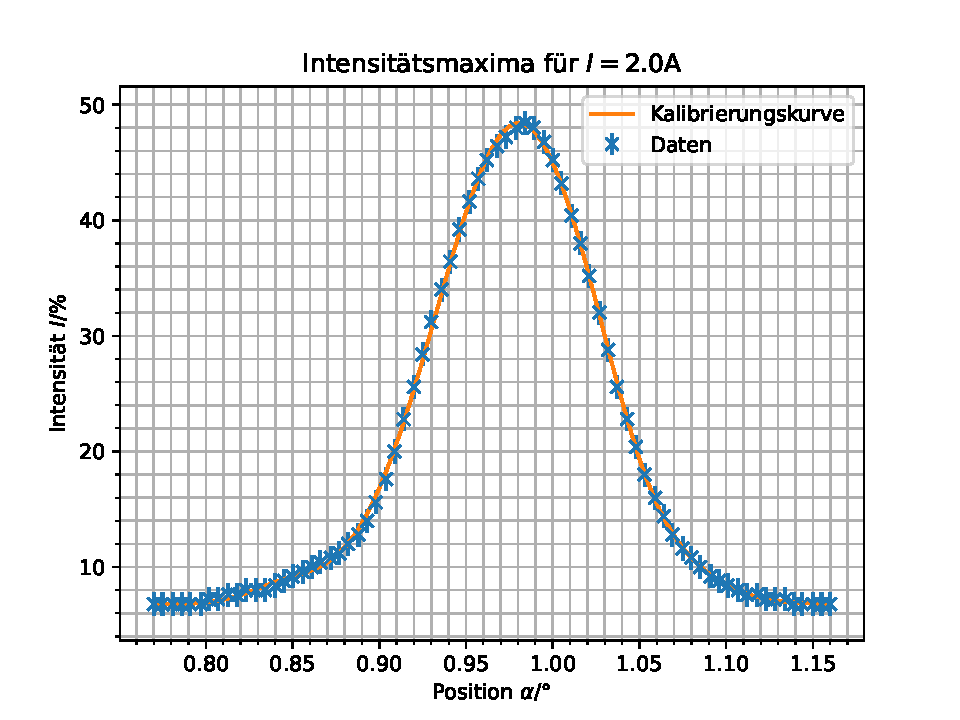
\includegraphics[width=\linewidth]{gauss_2.0A.pdf}
  \end{minipage}
  \hfill
  \begin{minipage}{.49\linewidth}
    \centering
    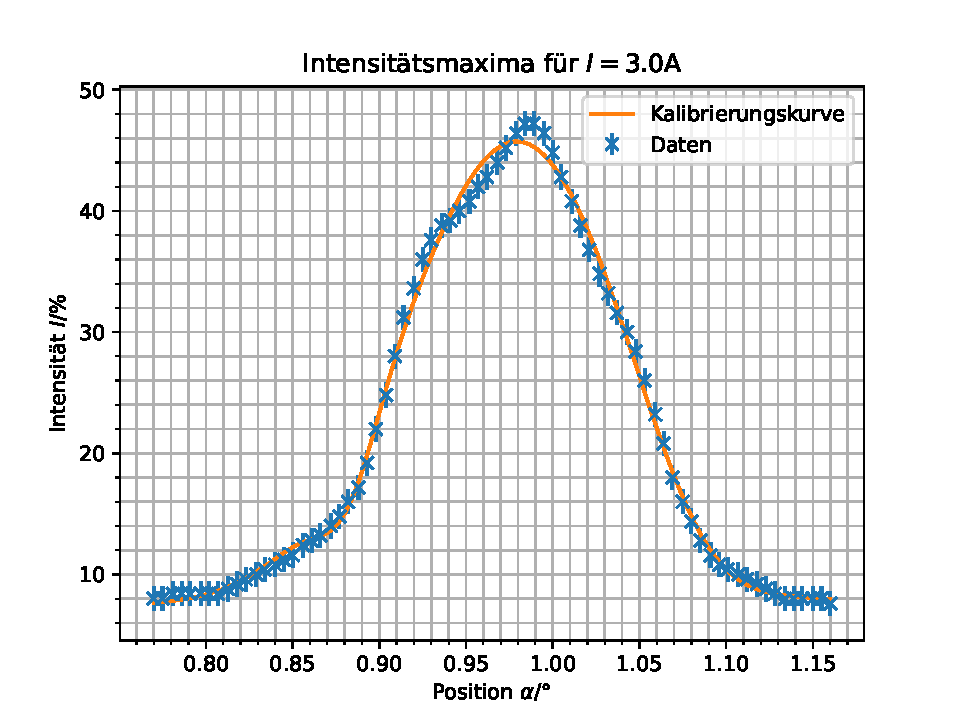
\includegraphics[width=\linewidth]{gauss_3.0A.pdf}
  \end{minipage}

  \begin{minipage}{.49\linewidth}
    \centering
    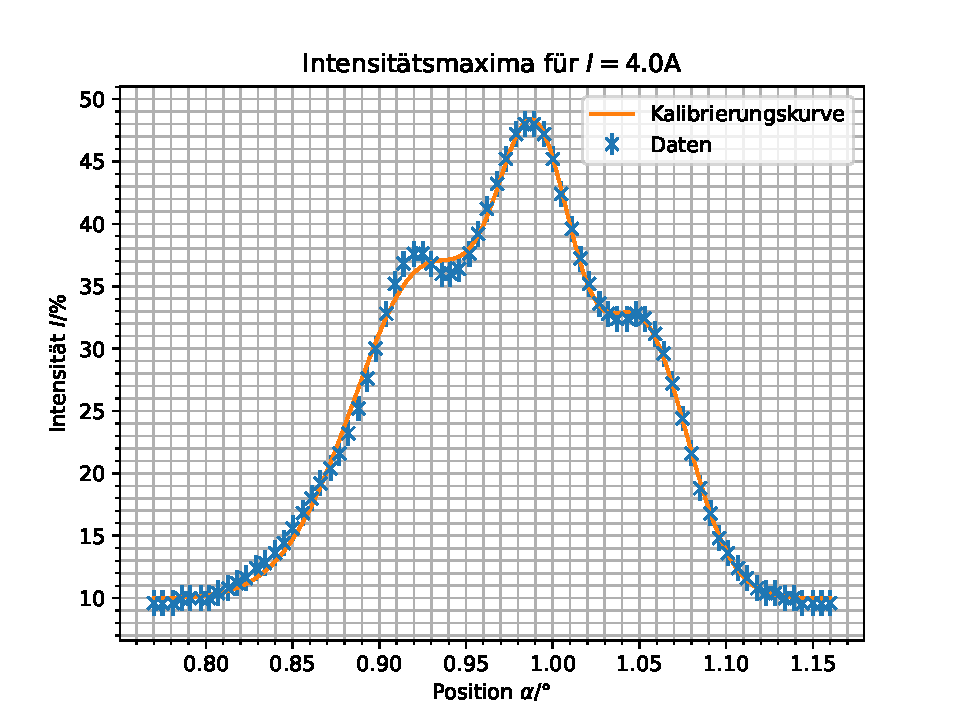
\includegraphics[width=\linewidth]{gauss_4.0A.pdf}
  \end{minipage}
  \hfill
  \begin{minipage}{.49\linewidth}
    \centering
    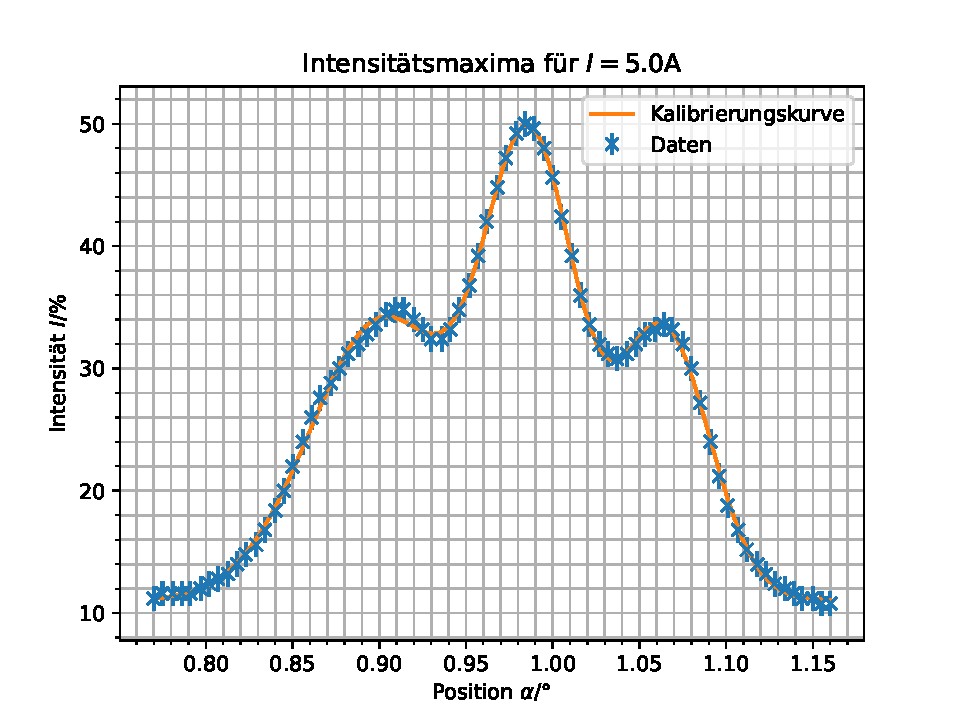
\includegraphics[width=\linewidth]{gauss_5.0A.pdf}
  \end{minipage}

  \begin{minipage}{.49\linewidth}
    \centering
    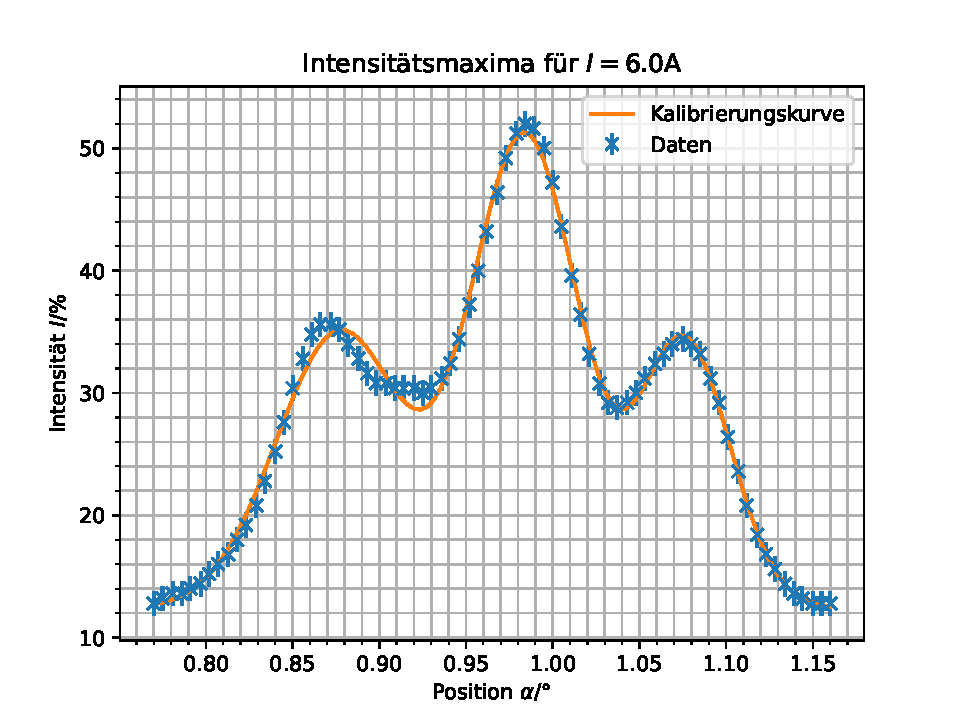
\includegraphics[width=\linewidth]{gauss_6.0A.pdf}
  \end{minipage}
  \hfill
  \begin{minipage}{.49\linewidth}
    \centering
    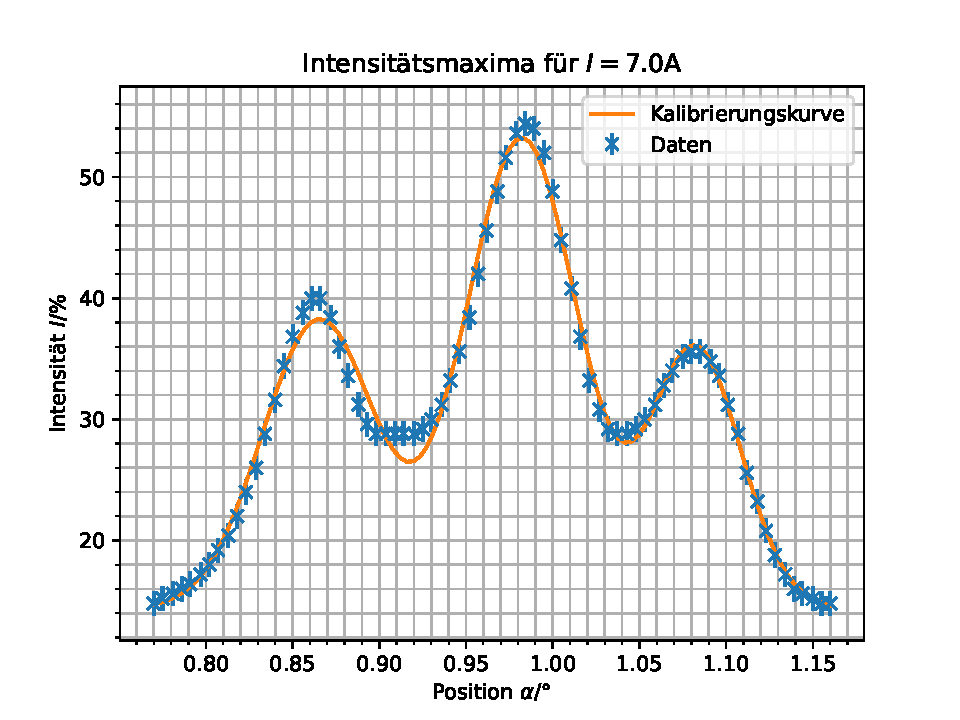
\includegraphics[width=\linewidth]{gauss_7.0A.pdf}
  \end{minipage}
  \caption{Ausgewählte Intensitätsmaxima für verschiedene Magnetströme $I$, mit Gauß-Fit [Teil 1]}
  \label{fig:gauss-fit-1}
\end{figure}

\begin{figure}[h]
  \centering
  \begin{minipage}{.49\linewidth}
    \centering
    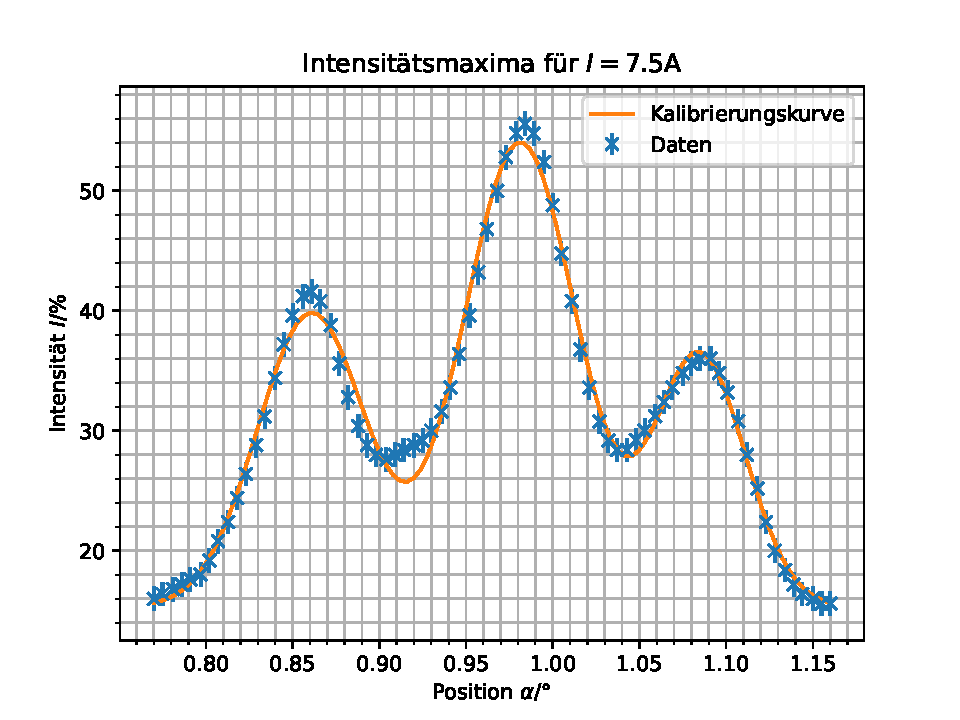
\includegraphics[width=\linewidth]{gauss_7.5A.pdf}
  \end{minipage}
  \hfill
  \begin{minipage}{.49\linewidth}
    \centering
    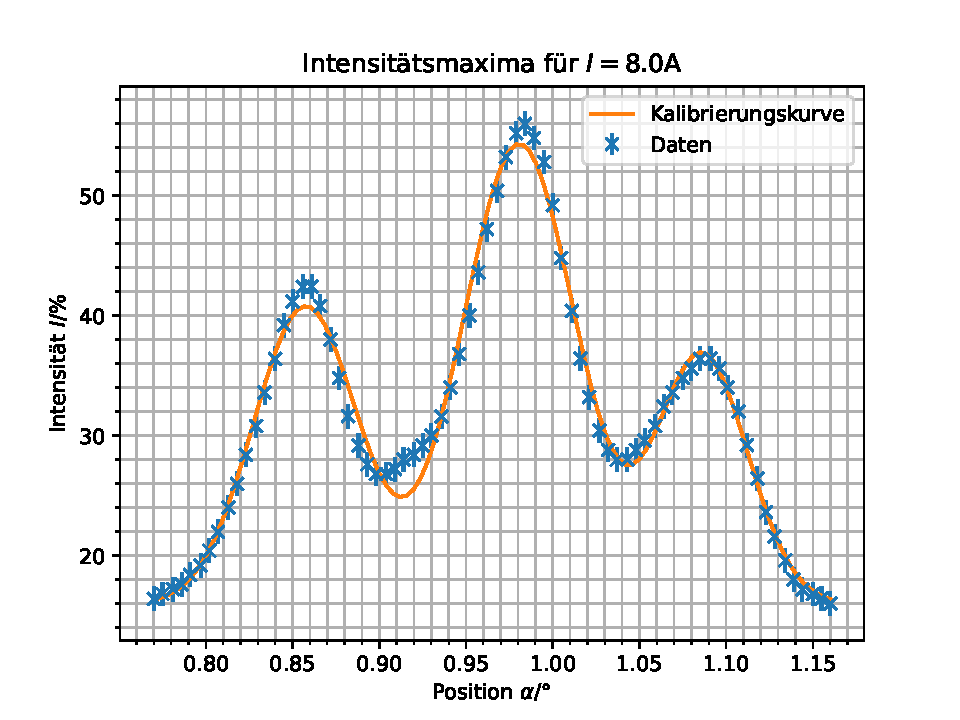
\includegraphics[width=\linewidth]{gauss_8.0A.pdf}
  \end{minipage}

  \begin{minipage}{.49\linewidth}
    \centering
    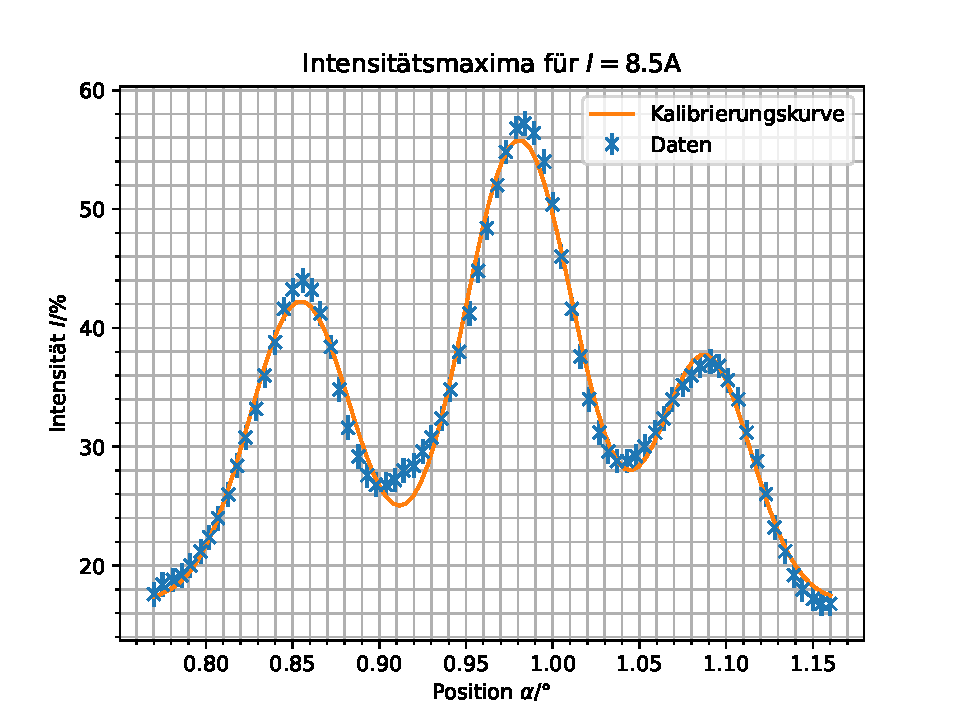
\includegraphics[width=\linewidth]{gauss_8.5A.pdf}
  \end{minipage}
  \hfill
  \begin{minipage}{.49\linewidth}
    \centering
    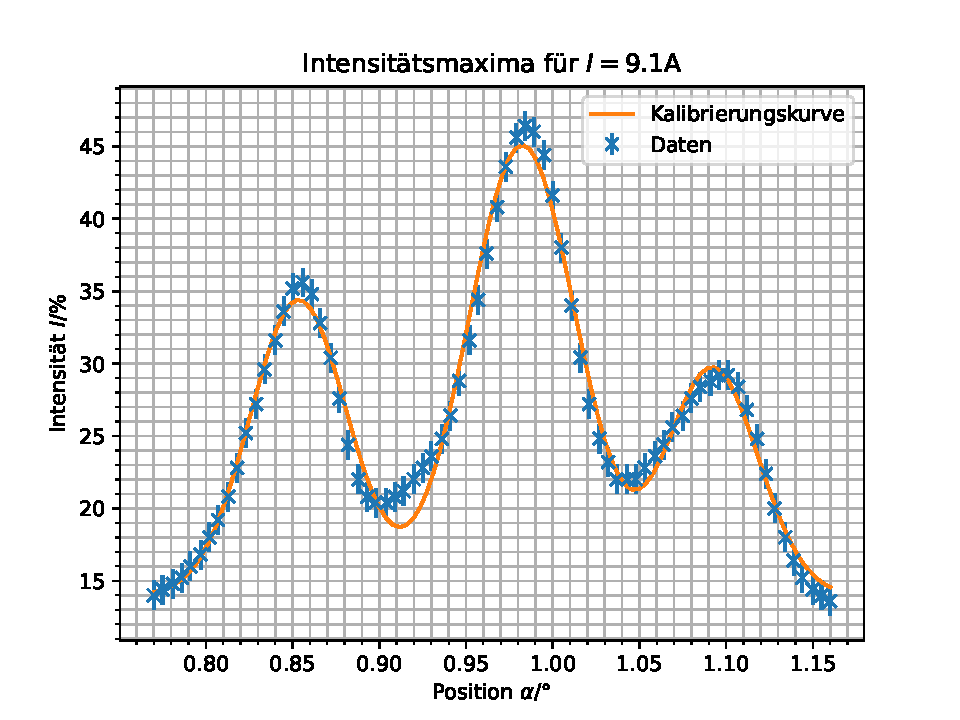
\includegraphics[width=\linewidth]{gauss_9.1A.pdf}
  \end{minipage}
  \caption{Ausgewählte Intensitätsmaxima für verschiedene Magnetströme $I$, mit Gauß-Fit [Teil 2]}
  \label{fig:gauss-fit-2}
\end{figure}

\begin{table}[h]
  \centering
  % \begin{tabular}{S[table-format=1.2] S[table-format=2.2] S[table-format=1.2] S[table-format=1.3] S[table-format=1.3] S[table-format=1.3] S[table-format=1.3]}
  \begin{tabular}{|ccccccc|}
    \toprule
    {$I/\si{A}$} & {$\mu_1/\si{\degree}$} & {$\Delta \mu_1/\si{\degree}$} & {$\mu_2/\si{\degree}$} & {$\Delta \mu_2/\si{\degree}$} & {$\mu_3/\si{\degree}$} & {$\Delta \mu_3/\si{\degree}$} \\
    \midrule
      2.00 & 1.46 & 0.14 & 0.85 & 0.0025 & 0.021 & 0.0026 \\
      3.00 & -4.67 & 0.74 & 0.88 & 0.0019 & 0.017 & 0.0029 \\
      4.00 & 26.43 & 0.43 & 0.93 & 0.0020 & 0.042 & 0.0015 \\
      5.00 & 22.97 & 0.18 & 0.90 & 0.00075 & 0.042 & 0.00073 \\
      6.00 & 22.62 & 0.38 & 0.88 & 0.00083 & 0.037 & 0.0011 \\
      7.00 & 23.84 & 0.56 & 0.87 & 0.00077 & 0.033 & 0.0011 \\
      7.50 & 24.48 & 0.62 & 0.86 & 0.00074 & 0.031 & 0.0011 \\
      8.00 & 24.80 & 0.66 & 0.86 & 0.00072 & 0.030 & 0.0010 \\
      8.50 & 25.29 & 0.69 & 0.85 & 0.00070 & 0.030 & 0.0010 \\
      9.10 & 20.42 & 0.63 & 0.85 & 0.00074 & 0.028 & 0.0011 \\
    \bottomrule
  \end{tabular}
  \caption{Bestimmte Parameter der Intensitätsmaxima für verschiedene Ströme. $\Delta I=\SI{0.2}{\A}$}
  \label{tab:parameter}
\end{table}
\clearpage
\begin{figure}[H]
  \centering
  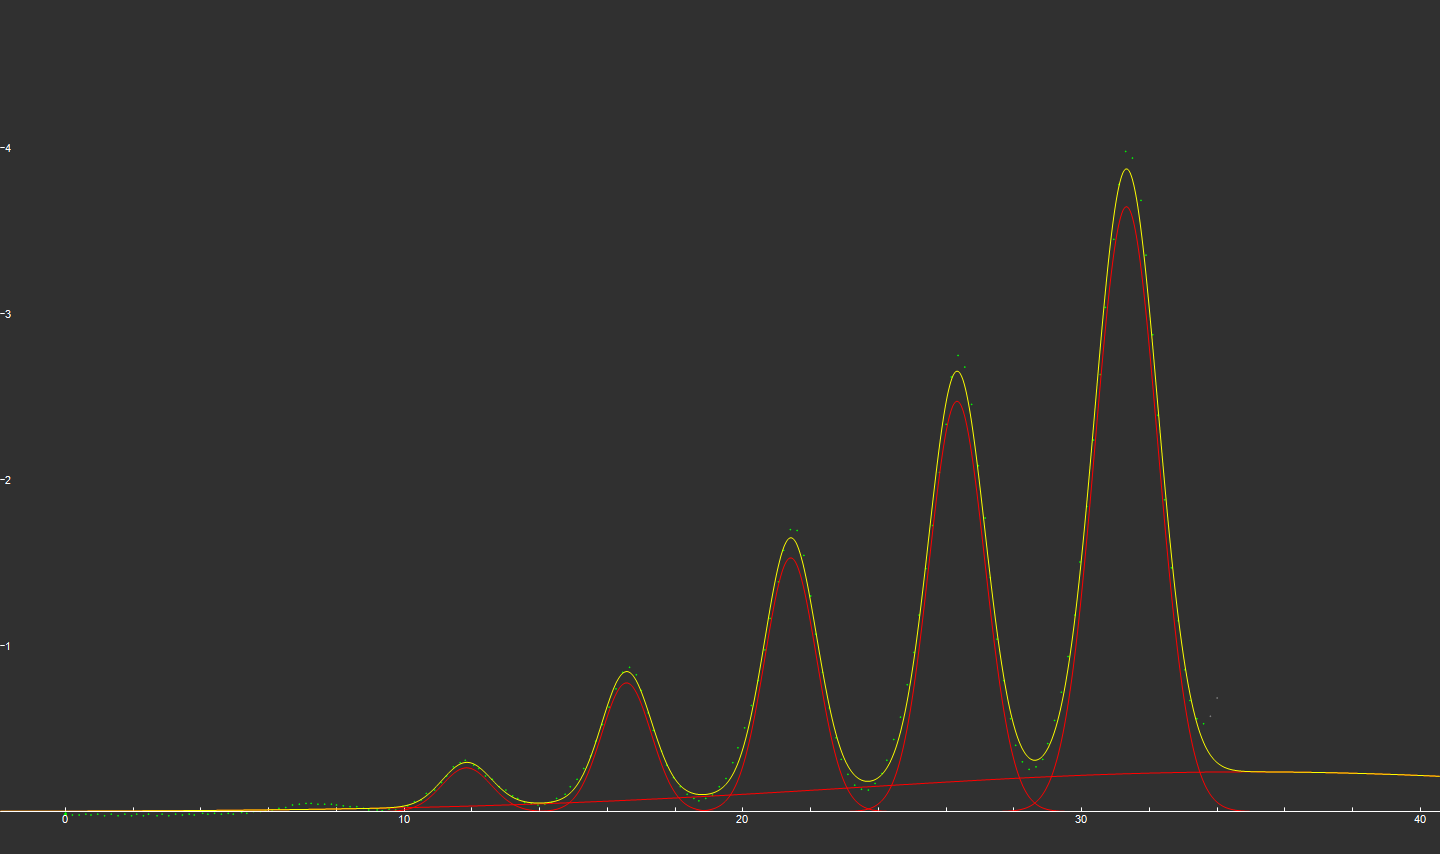
\includegraphics[scale=0.2]{FH_2,7V_165C.png}
  \caption{Gauß-Fit aus Fityk, Auftragung Anodenspannung $U_A$ gegen Beschleunigungsspannung $U_B$ bei $U_G=2,0$ und $T=165C$. Die gelbe
  Linie beschriebt die Summe aller Gauß-Fits und die Roten repräsentieren die einzelnen Fits.}
  \label{FH 2,7V_165C}
\end{figure}

\begin{figure}[H]
  \centering
  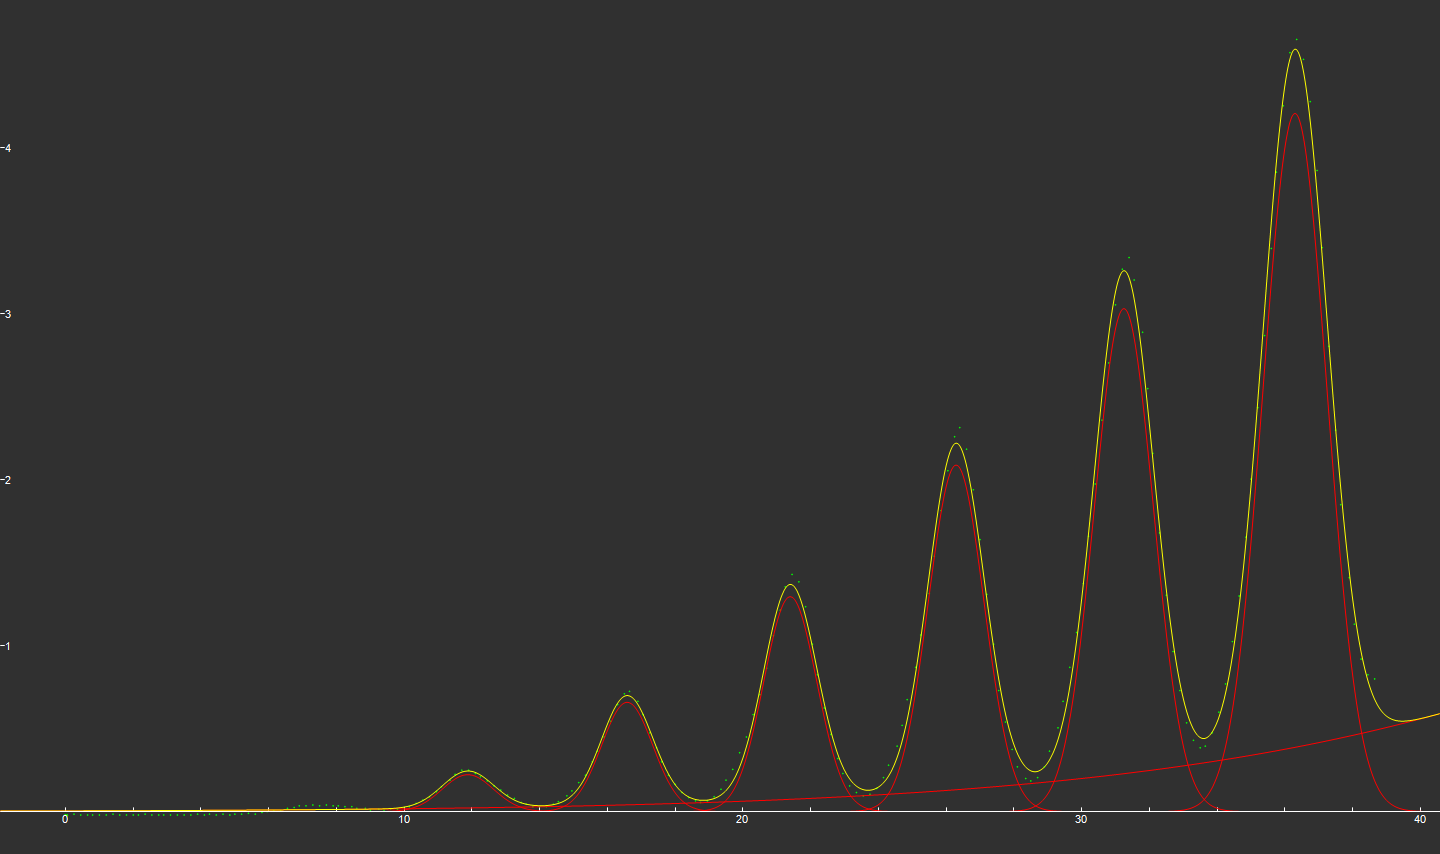
\includegraphics[scale=0.2]{FH_2,7V_170C.png}
  \caption{Gauß-Fit aus Fityk, Auftragung Anodenspannung $U_A$ gegen Beschleunigungsspannung $U_B$ bei $U_G=2,0$ und $T=170C$. Die gelbe
  Linie beschriebt die Summe aller Gauß-Fits und die Roten repräsentieren die einzelnen Fits.}
  \label{FH 2,0V_170C}
\end{figure}
\begin{figure}[H]
  \centering
  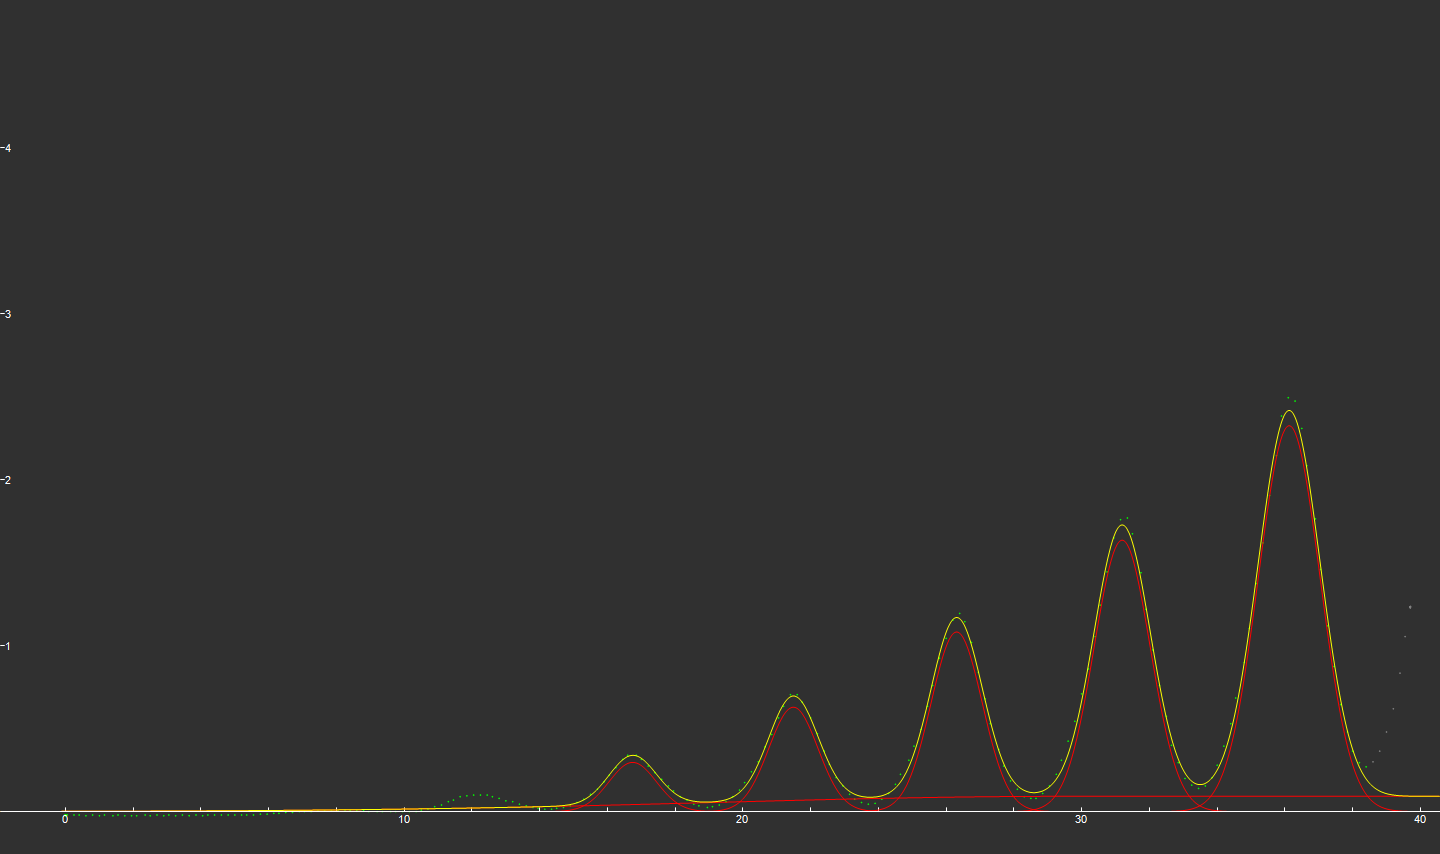
\includegraphics[scale=0.2]{FH_2,7V_175C.png}
  \caption{Gauß-Fit aus Fityk, Auftragung Anodenspannung $U_A$ gegen Beschleunigungsspannung $U_B$ bei $U_G=2,0$ und $T=175C$. Die gelbe
  Linie beschriebt die Summe aller Gauß-Fits und die Roten repräsentieren die einzelnen Fits.}
  \label{FH 2,0V_175C}
\end{figure}
\begin{figure}[H]
  \centering
  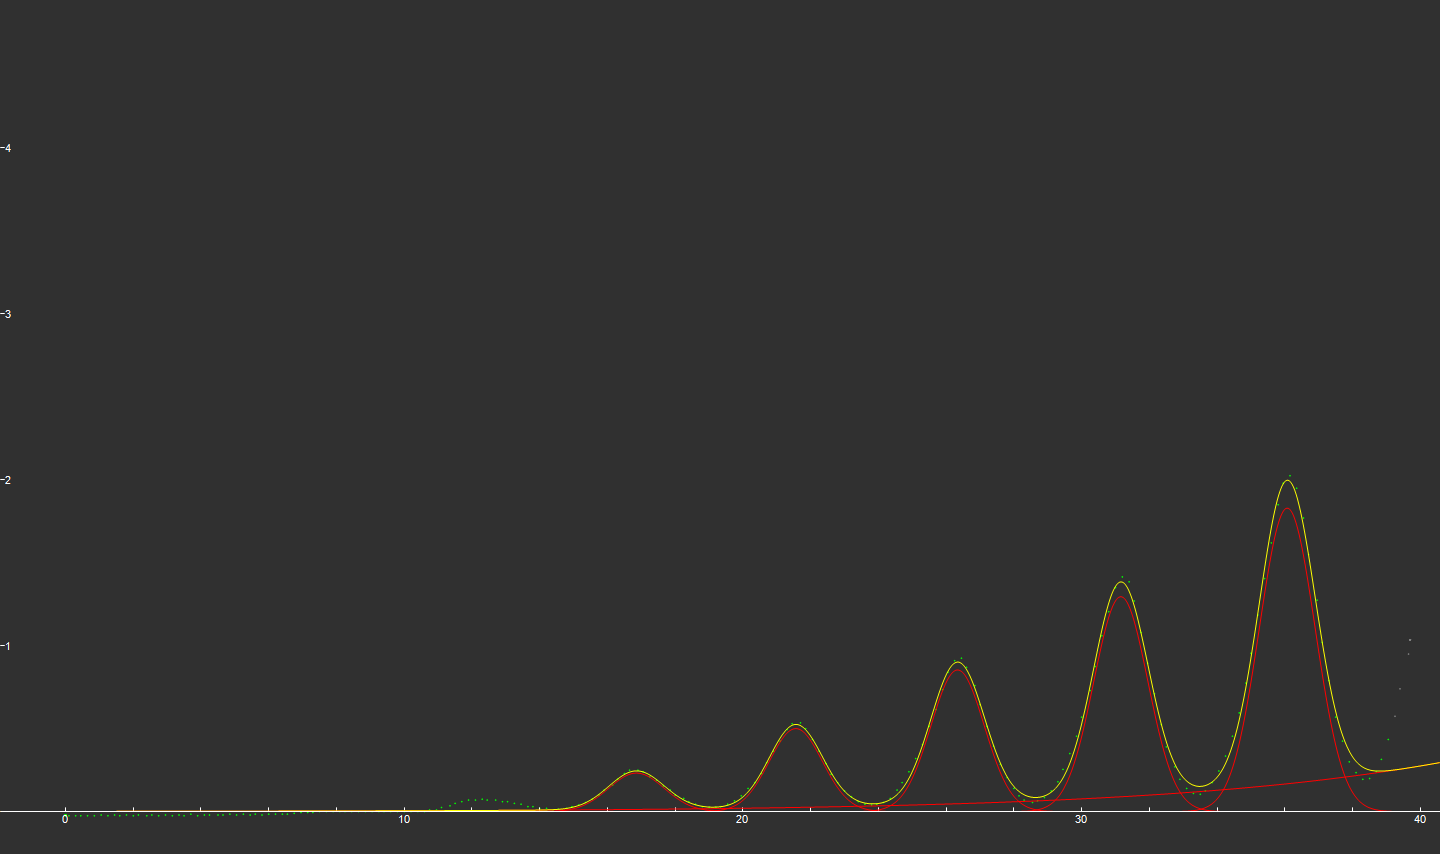
\includegraphics[scale=0.2]{FH_2,7V_180C.png}
  \caption{Gauß-Fit aus Fityk, Auftragung Anodenspannung $U_A$ gegen Beschleunigungsspannung $U_B$ bei $U_G=2,0$ und $T=180C$. Die gelbe
  Linie beschriebt die Summe aller Gauß-Fits und die Roten repräsentieren die einzelnen Fits.}
  \label{FH 2,0V_180C}
\end{figure}

\begin{figure}[H]
  \centering
  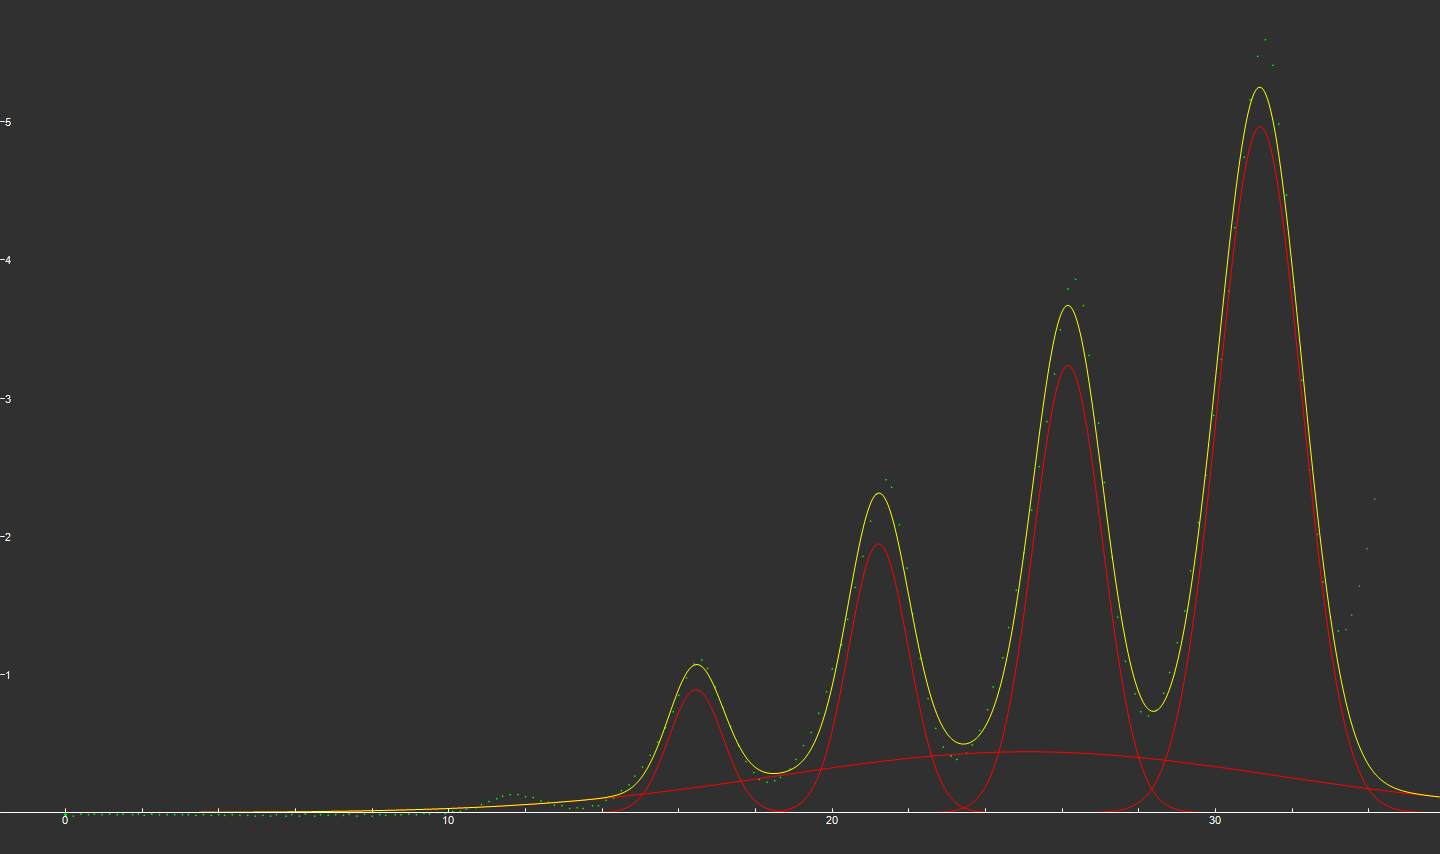
\includegraphics[scale=0.2]{FH_2,0V_165C.png}
  \caption{Gauß-Fit aus Fityk, Auftragung Anodenspannung $U_A$ gegen Beschleunigungsspannung $U_B$ bei $U_G=2,0$ und $T=165C$. Die gelbe
  Linie beschriebt die Summe aller Gauß-Fits und die Roten repräsentieren die einzelnen Fits.}
  \label{FH 2,7V_165C}
\end{figure}

\begin{figure}[H]
  \centering
  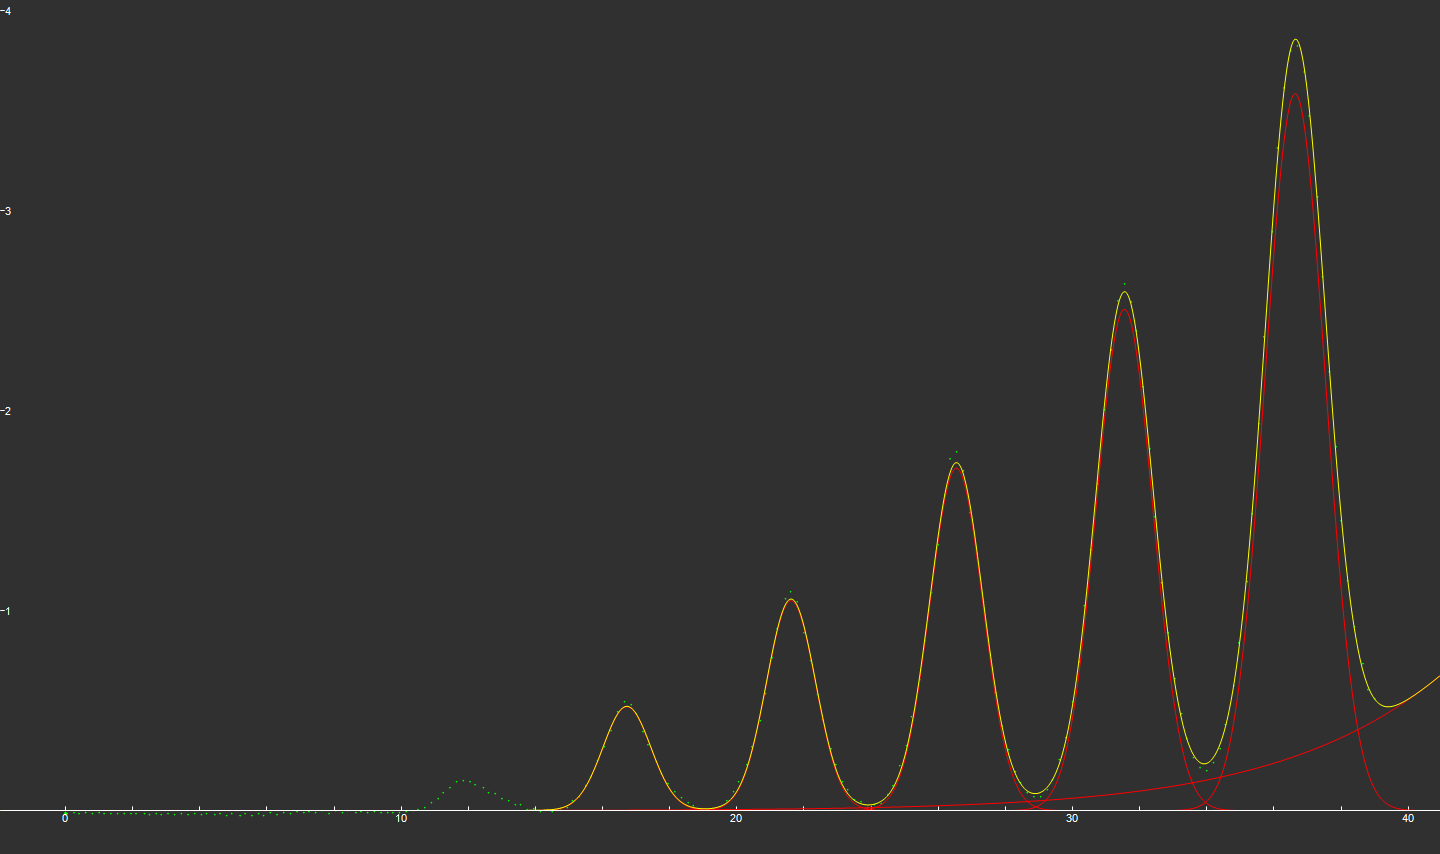
\includegraphics[scale=0.2]{FH_3,4_165C.png}
  \caption{Gauß-Fit aus Fityk, Auftragung Anodenspannung $U_A$ gegen Beschleunigungsspannung $U_B$ bei $U_G=3,4$ und $T=165C$. Die gelbe
  Linie beschriebt die Summe aller Gauß-Fits und die Roten repräsentieren die einzelnen Fits.}
  \label{FH 3,4V_165C}
\end{figure}

\begin{figure}[H]
  \centering
  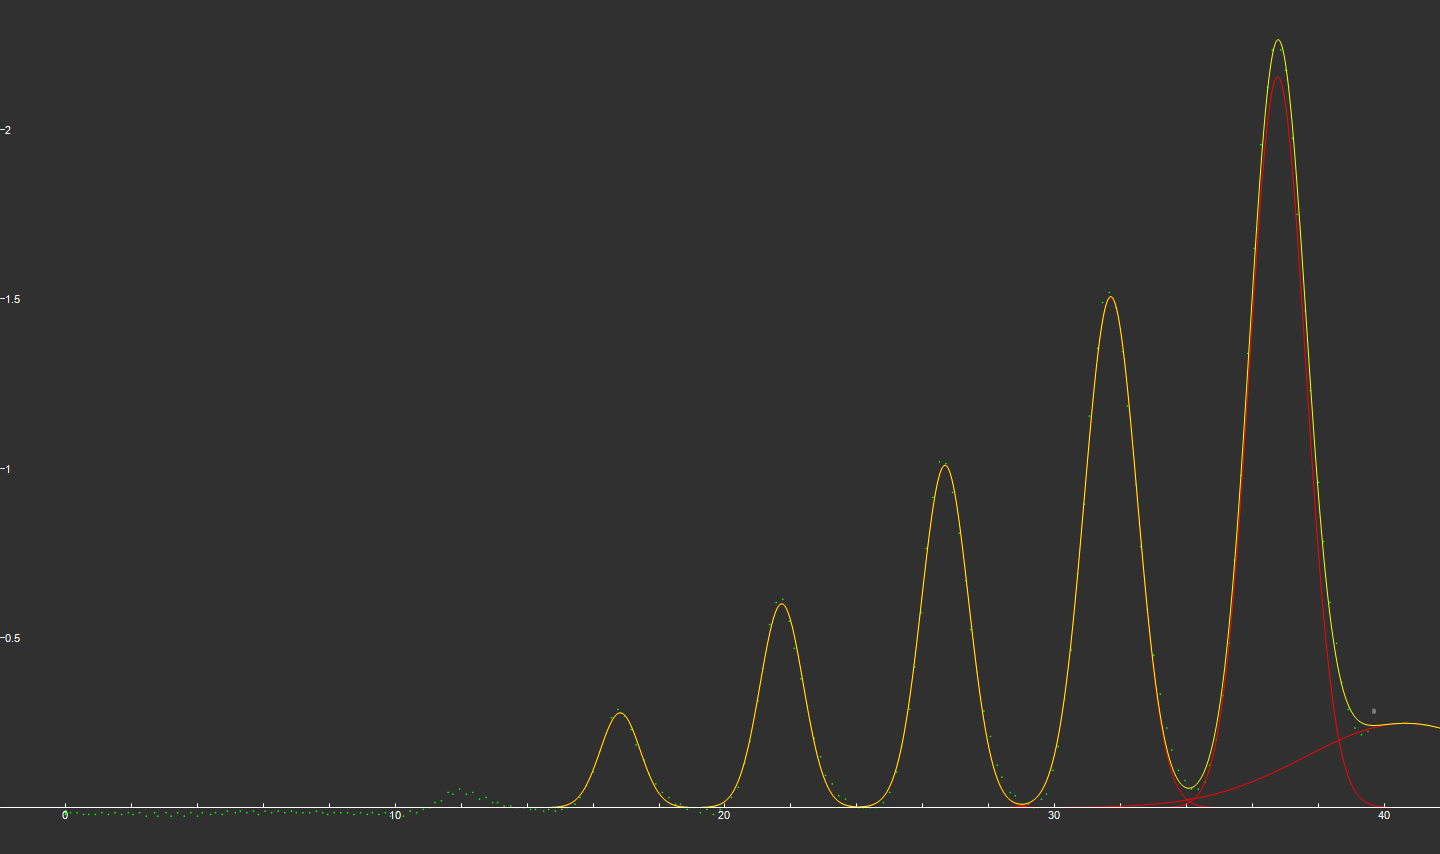
\includegraphics[scale=0.2]{FH_4,0V_165C.png}
  \caption{Gauß-Fit aus Fityk, Auftragung Anodenspannung $U_A$ gegen Beschleunigungsspannung $U_B$ bei $U_G=4,0$ und $T=165C$}
  \label{FH 4,0V_165C}
\end{figure}
\newpage
\begin{thebibliography}{9}

\bibitem{Anleitung}
\textit{Physikalisches Praktikum Teil IV -- Versuchsbeschreibungen}, Universität Bonn, Abruf 29.10.2024

\bibitem{Leybold}
\textit{Beobachtung des normalen Zeeman-Effekts in transversaler und longitudinaler Konfiguration}, Leybold Didactic, Abruf 30.10.2024

\bibitem{einheit}
\textit{Physics LibreTexts. (n.d.). 4.2: Measuring Motion - the Doppler Shift. , Abruf 05.11.2024}
\label{einheit}

\bibitem{bohr-magneton}
NIST, https://physics.nist.gov/cgi-bin/cuu/Value?mub, Abruf 15.11.2024

\bibitem{demtröder3}
\textit{Experimentalphysik 3 -- Atome, Moleküle, Festkörper}, 5. Auflage, Wolfgang Demtröder, 2016

\bibitem{chemistry}
\textit{Standard Atomic Weights}, CIAWW, https://www.ciaaw.org/atomic-weights.htm, Abruf 18.11.2024

\end{thebibliography}


\end{document}

